% Created by tikzDevice version 0.12 on 2019-05-09 12:20:12
% !TEX encoding = UTF-8 Unicode
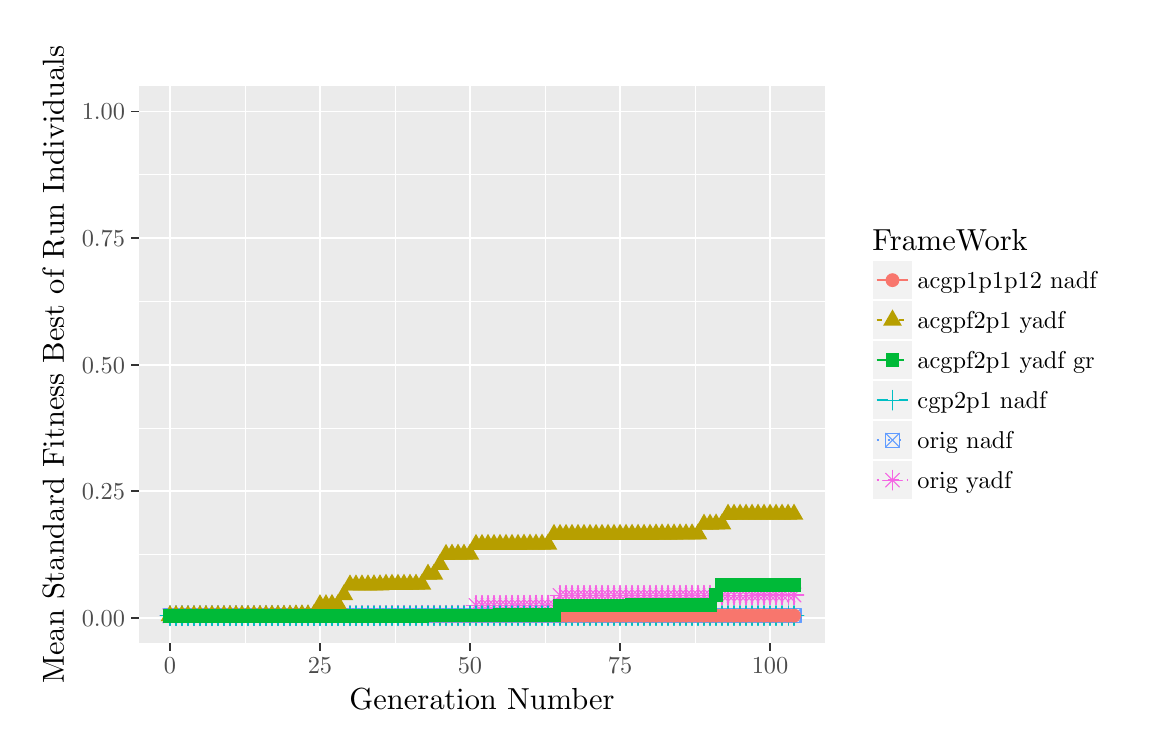
\begin{tikzpicture}[x=1pt,y=1pt]
\definecolor{fillColor}{RGB}{255,255,255}
\path[use as bounding box,fill=fillColor,fill opacity=0.00] (0,0) rectangle (397.48,252.94);
\begin{scope}
\path[clip] (  0.00,  0.00) rectangle (397.48,252.94);
\definecolor{drawColor}{RGB}{255,255,255}
\definecolor{fillColor}{RGB}{255,255,255}

\path[draw=drawColor,line width= 0.6pt,line join=round,line cap=round,fill=fillColor] (  0.00,  0.00) rectangle (397.48,252.95);
\end{scope}
\begin{scope}
\path[clip] ( 40.14, 30.56) rectangle (288.20,231.75);
\definecolor{fillColor}{gray}{0.92}

\path[fill=fillColor] ( 40.14, 30.56) rectangle (288.20,231.75);
\definecolor{drawColor}{RGB}{255,255,255}

\path[draw=drawColor,line width= 0.3pt,line join=round] ( 40.14, 62.57) --
	(288.20, 62.57);

\path[draw=drawColor,line width= 0.3pt,line join=round] ( 40.14,108.29) --
	(288.20,108.29);

\path[draw=drawColor,line width= 0.3pt,line join=round] ( 40.14,154.02) --
	(288.20,154.02);

\path[draw=drawColor,line width= 0.3pt,line join=round] ( 40.14,199.75) --
	(288.20,199.75);

\path[draw=drawColor,line width= 0.3pt,line join=round] ( 78.52, 30.56) --
	( 78.52,231.75);

\path[draw=drawColor,line width= 0.3pt,line join=round] (132.73, 30.56) --
	(132.73,231.75);

\path[draw=drawColor,line width= 0.3pt,line join=round] (186.94, 30.56) --
	(186.94,231.75);

\path[draw=drawColor,line width= 0.3pt,line join=round] (241.15, 30.56) --
	(241.15,231.75);

\path[draw=drawColor,line width= 0.6pt,line join=round] ( 40.14, 39.70) --
	(288.20, 39.70);

\path[draw=drawColor,line width= 0.6pt,line join=round] ( 40.14, 85.43) --
	(288.20, 85.43);

\path[draw=drawColor,line width= 0.6pt,line join=round] ( 40.14,131.16) --
	(288.20,131.16);

\path[draw=drawColor,line width= 0.6pt,line join=round] ( 40.14,176.88) --
	(288.20,176.88);

\path[draw=drawColor,line width= 0.6pt,line join=round] ( 40.14,222.61) --
	(288.20,222.61);

\path[draw=drawColor,line width= 0.6pt,line join=round] ( 51.41, 30.56) --
	( 51.41,231.75);

\path[draw=drawColor,line width= 0.6pt,line join=round] (105.62, 30.56) --
	(105.62,231.75);

\path[draw=drawColor,line width= 0.6pt,line join=round] (159.83, 30.56) --
	(159.83,231.75);

\path[draw=drawColor,line width= 0.6pt,line join=round] (214.04, 30.56) --
	(214.04,231.75);

\path[draw=drawColor,line width= 0.6pt,line join=round] (268.25, 30.56) --
	(268.25,231.75);
\definecolor{drawColor}{RGB}{248,118,109}

\path[draw=drawColor,line width= 0.6pt,line join=round] ( 51.41, 40.44) --
	( 53.58, 40.44) --
	( 55.75, 40.44) --
	( 57.92, 40.44) --
	( 60.09, 40.44) --
	( 62.26, 40.44) --
	( 64.42, 40.44) --
	( 66.59, 40.44) --
	( 68.76, 40.44) --
	( 70.93, 40.44) --
	( 73.10, 40.44) --
	( 75.27, 40.44) --
	( 77.43, 40.44) --
	( 79.60, 40.44) --
	( 81.77, 40.45) --
	( 83.94, 40.45) --
	( 86.11, 40.45) --
	( 88.28, 40.45) --
	( 90.44, 40.45) --
	( 92.61, 40.45) --
	( 94.78, 40.45) --
	( 96.95, 40.45) --
	( 99.12, 40.45) --
	(101.29, 40.45) --
	(103.45, 40.45) --
	(105.62, 40.45) --
	(107.79, 40.45) --
	(109.96, 40.45) --
	(112.13, 40.45) --
	(114.30, 40.45) --
	(116.47, 40.45) --
	(118.63, 40.45) --
	(120.80, 40.45) --
	(122.97, 40.45) --
	(125.14, 40.45) --
	(127.31, 40.46) --
	(129.48, 40.46) --
	(131.64, 40.46) --
	(133.81, 40.46) --
	(135.98, 40.46) --
	(138.15, 40.46) --
	(140.32, 40.46) --
	(142.49, 40.46) --
	(144.65, 40.46) --
	(146.82, 40.46) --
	(148.99, 40.46) --
	(151.16, 40.46) --
	(153.33, 40.46) --
	(155.50, 40.46) --
	(157.66, 40.46) --
	(159.83, 40.46) --
	(162.00, 40.46) --
	(164.17, 40.46) --
	(166.34, 40.46) --
	(168.51, 40.46) --
	(170.67, 40.46) --
	(172.84, 40.46) --
	(175.01, 40.46) --
	(177.18, 40.46) --
	(179.35, 40.46) --
	(181.52, 40.46) --
	(183.68, 40.46) --
	(185.85, 40.46) --
	(188.02, 40.46) --
	(190.19, 40.46) --
	(192.36, 40.46) --
	(194.53, 40.46) --
	(196.69, 40.46) --
	(198.86, 40.46) --
	(201.03, 40.47) --
	(203.20, 40.47) --
	(205.37, 40.47) --
	(207.54, 40.47) --
	(209.70, 40.47) --
	(211.87, 40.47) --
	(214.04, 40.47) --
	(216.21, 40.47) --
	(218.38, 40.47) --
	(220.55, 40.47) --
	(222.72, 40.47) --
	(224.88, 40.47) --
	(227.05, 40.47) --
	(229.22, 40.47) --
	(231.39, 40.47) --
	(233.56, 40.47) --
	(235.73, 40.47) --
	(237.89, 40.47) --
	(240.06, 40.47) --
	(242.23, 40.47) --
	(244.40, 40.47) --
	(246.57, 40.47) --
	(248.74, 40.47) --
	(250.90, 40.47) --
	(253.07, 40.47) --
	(255.24, 40.47) --
	(257.41, 40.47) --
	(259.58, 40.47) --
	(261.75, 40.47) --
	(263.91, 40.47) --
	(266.08, 40.47) --
	(268.25, 40.47) --
	(270.42, 40.47) --
	(272.59, 40.47) --
	(274.76, 40.47) --
	(276.92, 40.47);
\definecolor{drawColor}{RGB}{183,159,0}

\path[draw=drawColor,line width= 0.6pt,dash pattern=on 2pt off 2pt ,line join=round] ( 51.41, 40.44) --
	( 53.58, 40.44) --
	( 55.75, 40.45) --
	( 57.92, 40.46) --
	( 60.09, 40.46) --
	( 62.26, 40.47) --
	( 64.42, 40.47) --
	( 66.59, 40.48) --
	( 68.76, 40.48) --
	( 70.93, 40.49) --
	( 73.10, 40.50) --
	( 75.27, 40.50) --
	( 77.43, 40.50) --
	( 79.60, 40.51) --
	( 81.77, 40.52) --
	( 83.94, 40.53) --
	( 86.11, 40.55) --
	( 88.28, 40.57) --
	( 90.44, 40.57) --
	( 92.61, 40.57) --
	( 94.78, 40.58) --
	( 96.95, 40.68) --
	( 99.12, 40.72) --
	(101.29, 40.73) --
	(103.45, 40.77) --
	(105.62, 44.37) --
	(107.79, 44.38) --
	(109.96, 44.46) --
	(112.13, 44.46) --
	(114.30, 47.98) --
	(116.47, 51.51) --
	(118.63, 51.52) --
	(120.80, 51.52) --
	(122.97, 51.52) --
	(125.14, 51.57) --
	(127.31, 51.59) --
	(129.48, 51.75) --
	(131.64, 51.75) --
	(133.81, 51.76) --
	(135.98, 51.76) --
	(138.15, 51.79) --
	(140.32, 51.79) --
	(142.49, 51.79) --
	(144.65, 55.39) --
	(146.82, 55.39) --
	(148.99, 58.94) --
	(151.16, 62.55) --
	(153.33, 62.62) --
	(155.50, 62.62) --
	(157.66, 62.62) --
	(159.83, 62.62) --
	(162.00, 66.15) --
	(164.17, 66.15) --
	(166.34, 66.16) --
	(168.51, 66.16) --
	(170.67, 66.16) --
	(172.84, 66.19) --
	(175.01, 66.19) --
	(177.18, 66.19) --
	(179.35, 66.26) --
	(181.52, 66.26) --
	(183.68, 66.26) --
	(185.85, 66.26) --
	(188.02, 66.26) --
	(190.19, 69.78) --
	(192.36, 69.78) --
	(194.53, 69.78) --
	(196.69, 69.78) --
	(198.86, 69.78) --
	(201.03, 69.78) --
	(203.20, 69.79) --
	(205.37, 69.79) --
	(207.54, 69.80) --
	(209.70, 69.80) --
	(211.87, 69.80) --
	(214.04, 69.80) --
	(216.21, 69.81) --
	(218.38, 69.82) --
	(220.55, 69.82) --
	(222.72, 69.83) --
	(224.88, 69.83) --
	(227.05, 69.94) --
	(229.22, 69.94) --
	(231.39, 69.94) --
	(233.56, 69.94) --
	(235.73, 69.96) --
	(237.89, 69.96) --
	(240.06, 69.96) --
	(242.23, 69.96) --
	(244.40, 73.48) --
	(246.57, 73.48) --
	(248.74, 73.55) --
	(250.90, 73.55) --
	(253.07, 77.07) --
	(255.24, 77.07) --
	(257.41, 77.07) --
	(259.58, 77.07) --
	(261.75, 77.08) --
	(263.91, 77.08) --
	(266.08, 77.08) --
	(268.25, 77.09) --
	(270.42, 77.09) --
	(272.59, 77.09) --
	(274.76, 77.09) --
	(276.92, 77.09);
\definecolor{drawColor}{RGB}{0,186,56}

\path[draw=drawColor,line width= 0.6pt,dash pattern=on 4pt off 2pt ,line join=round] ( 51.41, 40.44) --
	( 53.58, 40.44) --
	( 55.75, 40.44) --
	( 57.92, 40.44) --
	( 60.09, 40.44) --
	( 62.26, 40.44) --
	( 64.42, 40.45) --
	( 66.59, 40.45) --
	( 68.76, 40.45) --
	( 70.93, 40.45) --
	( 73.10, 40.45) --
	( 75.27, 40.45) --
	( 77.43, 40.45) --
	( 79.60, 40.45) --
	( 81.77, 40.46) --
	( 83.94, 40.46) --
	( 86.11, 40.46) --
	( 88.28, 40.46) --
	( 90.44, 40.47) --
	( 92.61, 40.47) --
	( 94.78, 40.47) --
	( 96.95, 40.47) --
	( 99.12, 40.47) --
	(101.29, 40.47) --
	(103.45, 40.47) --
	(105.62, 40.48) --
	(107.79, 40.48) --
	(109.96, 40.48) --
	(112.13, 40.48) --
	(114.30, 40.48) --
	(116.47, 40.48) --
	(118.63, 40.48) --
	(120.80, 40.48) --
	(122.97, 40.48) --
	(125.14, 40.48) --
	(127.31, 40.48) --
	(129.48, 40.48) --
	(131.64, 40.48) --
	(133.81, 40.48) --
	(135.98, 40.49) --
	(138.15, 40.49) --
	(140.32, 40.49) --
	(142.49, 40.49) --
	(144.65, 40.49) --
	(146.82, 40.49) --
	(148.99, 40.50) --
	(151.16, 40.50) --
	(153.33, 40.51) --
	(155.50, 40.51) --
	(157.66, 40.51) --
	(159.83, 40.51) --
	(162.00, 40.52) --
	(164.17, 40.52) --
	(166.34, 40.55) --
	(168.51, 40.55) --
	(170.67, 40.61) --
	(172.84, 40.61) --
	(175.01, 40.61) --
	(177.18, 40.62) --
	(179.35, 40.62) --
	(181.52, 40.62) --
	(183.68, 40.62) --
	(185.85, 40.62) --
	(188.02, 40.62) --
	(190.19, 40.62) --
	(192.36, 44.14) --
	(194.53, 44.14) --
	(196.69, 44.14) --
	(198.86, 44.14) --
	(201.03, 44.15) --
	(203.20, 44.15) --
	(205.37, 44.15) --
	(207.54, 44.15) --
	(209.70, 44.15) --
	(211.87, 44.16) --
	(214.04, 44.17) --
	(216.21, 44.17) --
	(218.38, 44.18) --
	(220.55, 44.19) --
	(222.72, 44.19) --
	(224.88, 44.19) --
	(227.05, 44.22) --
	(229.22, 44.22) --
	(231.39, 44.25) --
	(233.56, 44.32) --
	(235.73, 44.32) --
	(237.89, 44.32) --
	(240.06, 44.32) --
	(242.23, 44.32) --
	(244.40, 44.32) --
	(246.57, 44.39) --
	(248.74, 47.91) --
	(250.90, 51.43) --
	(253.07, 51.43) --
	(255.24, 51.43) --
	(257.41, 51.43) --
	(259.58, 51.43) --
	(261.75, 51.43) --
	(263.91, 51.43) --
	(266.08, 51.43) --
	(268.25, 51.43) --
	(270.42, 51.43) --
	(272.59, 51.43) --
	(274.76, 51.43) --
	(276.92, 51.43);
\definecolor{drawColor}{RGB}{0,191,196}

\path[draw=drawColor,line width= 0.6pt,dash pattern=on 4pt off 4pt ,line join=round] ( 51.41, 40.44) --
	( 53.58, 40.44) --
	( 55.75, 40.44) --
	( 57.92, 40.44) --
	( 60.09, 40.44) --
	( 62.26, 40.44) --
	( 64.42, 40.44) --
	( 66.59, 40.44) --
	( 68.76, 40.45) --
	( 70.93, 40.45) --
	( 73.10, 40.45) --
	( 75.27, 40.45) --
	( 77.43, 40.45) --
	( 79.60, 40.45) --
	( 81.77, 40.45) --
	( 83.94, 40.45) --
	( 86.11, 40.45) --
	( 88.28, 40.45) --
	( 90.44, 40.45) --
	( 92.61, 40.45) --
	( 94.78, 40.45) --
	( 96.95, 40.45) --
	( 99.12, 40.45) --
	(101.29, 40.45) --
	(103.45, 40.45) --
	(105.62, 40.45) --
	(107.79, 40.46) --
	(109.96, 40.46) --
	(112.13, 40.46) --
	(114.30, 40.46) --
	(116.47, 40.46) --
	(118.63, 40.46) --
	(120.80, 40.46) --
	(122.97, 40.46) --
	(125.14, 40.46) --
	(127.31, 40.46) --
	(129.48, 40.46) --
	(131.64, 40.46) --
	(133.81, 40.46) --
	(135.98, 40.46) --
	(138.15, 40.46) --
	(140.32, 40.46) --
	(142.49, 40.46) --
	(144.65, 40.46) --
	(146.82, 40.46) --
	(148.99, 40.46) --
	(151.16, 40.46) --
	(153.33, 40.46) --
	(155.50, 40.46) --
	(157.66, 40.46) --
	(159.83, 40.46) --
	(162.00, 40.46) --
	(164.17, 40.46) --
	(166.34, 40.46) --
	(168.51, 40.47) --
	(170.67, 40.47) --
	(172.84, 40.47) --
	(175.01, 40.47) --
	(177.18, 40.47) --
	(179.35, 40.47) --
	(181.52, 40.47) --
	(183.68, 40.47) --
	(185.85, 40.47) --
	(188.02, 40.47) --
	(190.19, 40.47) --
	(192.36, 40.47) --
	(194.53, 40.47) --
	(196.69, 40.47) --
	(198.86, 40.47) --
	(201.03, 40.47) --
	(203.20, 40.47) --
	(205.37, 40.47) --
	(207.54, 40.47) --
	(209.70, 40.47) --
	(211.87, 40.47) --
	(214.04, 40.47) --
	(216.21, 40.47) --
	(218.38, 40.47) --
	(220.55, 40.47) --
	(222.72, 40.47) --
	(224.88, 40.47) --
	(227.05, 40.47) --
	(229.22, 40.47) --
	(231.39, 40.47) --
	(233.56, 40.47) --
	(235.73, 40.47) --
	(237.89, 40.47) --
	(240.06, 40.47) --
	(242.23, 40.47) --
	(244.40, 40.48) --
	(246.57, 40.48) --
	(248.74, 40.48) --
	(250.90, 40.48) --
	(253.07, 40.48) --
	(255.24, 40.48) --
	(257.41, 40.48) --
	(259.58, 40.48) --
	(261.75, 40.48) --
	(263.91, 40.48) --
	(266.08, 40.48) --
	(268.25, 40.48) --
	(270.42, 40.48) --
	(272.59, 40.48) --
	(274.76, 40.48) --
	(276.92, 40.48);
\definecolor{drawColor}{RGB}{97,156,255}

\path[draw=drawColor,line width= 0.6pt,dash pattern=on 1pt off 3pt ,line join=round] ( 51.41, 40.44) --
	( 53.58, 40.44) --
	( 55.75, 40.44) --
	( 57.92, 40.44) --
	( 60.09, 40.44) --
	( 62.26, 40.44) --
	( 64.42, 40.44) --
	( 66.59, 40.44) --
	( 68.76, 40.44) --
	( 70.93, 40.44) --
	( 73.10, 40.44) --
	( 75.27, 40.44) --
	( 77.43, 40.44) --
	( 79.60, 40.44) --
	( 81.77, 40.44) --
	( 83.94, 40.44) --
	( 86.11, 40.44) --
	( 88.28, 40.44) --
	( 90.44, 40.44) --
	( 92.61, 40.44) --
	( 94.78, 40.45) --
	( 96.95, 40.45) --
	( 99.12, 40.45) --
	(101.29, 40.45) --
	(103.45, 40.45) --
	(105.62, 40.45) --
	(107.79, 40.45) --
	(109.96, 40.45) --
	(112.13, 40.45) --
	(114.30, 40.45) --
	(116.47, 40.45) --
	(118.63, 40.45) --
	(120.80, 40.45) --
	(122.97, 40.45) --
	(125.14, 40.45) --
	(127.31, 40.45) --
	(129.48, 40.45) --
	(131.64, 40.45) --
	(133.81, 40.45) --
	(135.98, 40.45) --
	(138.15, 40.45) --
	(140.32, 40.45) --
	(142.49, 40.45) --
	(144.65, 40.45) --
	(146.82, 40.45) --
	(148.99, 40.45) --
	(151.16, 40.45) --
	(153.33, 40.45) --
	(155.50, 40.45) --
	(157.66, 40.45) --
	(159.83, 40.45) --
	(162.00, 40.45) --
	(164.17, 40.45) --
	(166.34, 40.45) --
	(168.51, 40.45) --
	(170.67, 40.45) --
	(172.84, 40.45) --
	(175.01, 40.45) --
	(177.18, 40.45) --
	(179.35, 40.45) --
	(181.52, 40.45) --
	(183.68, 40.45) --
	(185.85, 40.45) --
	(188.02, 40.45) --
	(190.19, 40.46) --
	(192.36, 40.46) --
	(194.53, 40.46) --
	(196.69, 40.46) --
	(198.86, 40.46) --
	(201.03, 40.46) --
	(203.20, 40.46) --
	(205.37, 40.46) --
	(207.54, 40.46) --
	(209.70, 40.46) --
	(211.87, 40.46) --
	(214.04, 40.46) --
	(216.21, 40.46) --
	(218.38, 40.46) --
	(220.55, 40.46) --
	(222.72, 40.46) --
	(224.88, 40.46) --
	(227.05, 40.46) --
	(229.22, 40.46) --
	(231.39, 40.46) --
	(233.56, 40.46) --
	(235.73, 40.46) --
	(237.89, 40.46) --
	(240.06, 40.46) --
	(242.23, 40.46) --
	(244.40, 40.46) --
	(246.57, 40.46) --
	(248.74, 40.46) --
	(250.90, 40.47) --
	(253.07, 40.47) --
	(255.24, 40.47) --
	(257.41, 40.47) --
	(259.58, 40.47) --
	(261.75, 40.47) --
	(263.91, 40.47) --
	(266.08, 40.47) --
	(268.25, 40.47) --
	(270.42, 40.47) --
	(272.59, 40.47) --
	(274.76, 40.47) --
	(276.92, 40.47);
\definecolor{drawColor}{RGB}{245,100,227}

\path[draw=drawColor,line width= 0.6pt,dash pattern=on 1pt off 3pt on 4pt off 3pt ,line join=round] ( 51.41, 40.44) --
	( 53.58, 40.44) --
	( 55.75, 40.44) --
	( 57.92, 40.44) --
	( 60.09, 40.45) --
	( 62.26, 40.45) --
	( 64.42, 40.46) --
	( 66.59, 40.47) --
	( 68.76, 40.47) --
	( 70.93, 40.47) --
	( 73.10, 40.47) --
	( 75.27, 40.48) --
	( 77.43, 40.48) --
	( 79.60, 40.48) --
	( 81.77, 40.48) --
	( 83.94, 40.48) --
	( 86.11, 40.49) --
	( 88.28, 40.50) --
	( 90.44, 40.50) --
	( 92.61, 40.50) --
	( 94.78, 40.50) --
	( 96.95, 40.50) --
	( 99.12, 40.50) --
	(101.29, 40.50) --
	(103.45, 40.51) --
	(105.62, 40.51) --
	(107.79, 40.51) --
	(109.96, 40.52) --
	(112.13, 40.53) --
	(114.30, 40.54) --
	(116.47, 40.54) --
	(118.63, 40.54) --
	(120.80, 40.54) --
	(122.97, 40.54) --
	(125.14, 40.54) --
	(127.31, 40.56) --
	(129.48, 40.56) --
	(131.64, 40.56) --
	(133.81, 40.56) --
	(135.98, 40.57) --
	(138.15, 40.57) --
	(140.32, 40.64) --
	(142.49, 40.64) --
	(144.65, 40.64) --
	(146.82, 40.64) --
	(148.99, 40.64) --
	(151.16, 40.64) --
	(153.33, 40.64) --
	(155.50, 40.64) --
	(157.66, 40.65) --
	(159.83, 40.66) --
	(162.00, 44.17) --
	(164.17, 44.18) --
	(166.34, 44.18) --
	(168.51, 44.19) --
	(170.67, 44.19) --
	(172.84, 44.19) --
	(175.01, 44.21) --
	(177.18, 44.21) --
	(179.35, 44.21) --
	(181.52, 44.21) --
	(183.68, 44.28) --
	(185.85, 44.28) --
	(188.02, 44.28) --
	(190.19, 44.29) --
	(192.36, 47.80) --
	(194.53, 47.80) --
	(196.69, 47.80) --
	(198.86, 47.80) --
	(201.03, 47.80) --
	(203.20, 47.80) --
	(205.37, 47.81) --
	(207.54, 47.81) --
	(209.70, 47.81) --
	(211.87, 47.81) --
	(214.04, 47.81) --
	(216.21, 47.81) --
	(218.38, 47.81) --
	(220.55, 47.81) --
	(222.72, 47.81) --
	(224.88, 47.81) --
	(227.05, 47.81) --
	(229.22, 47.81) --
	(231.39, 47.82) --
	(233.56, 47.82) --
	(235.73, 47.82) --
	(237.89, 47.82) --
	(240.06, 47.82) --
	(242.23, 47.82) --
	(244.40, 47.82) --
	(246.57, 47.86) --
	(248.74, 47.86) --
	(250.90, 47.86) --
	(253.07, 47.86) --
	(255.24, 47.86) --
	(257.41, 47.86) --
	(259.58, 47.86) --
	(261.75, 47.86) --
	(263.91, 47.86) --
	(266.08, 47.93) --
	(268.25, 47.93) --
	(270.42, 47.93) --
	(272.59, 47.93) --
	(274.76, 47.93) --
	(276.92, 47.93);
\definecolor{drawColor}{RGB}{97,156,255}

\path[draw=drawColor,line width= 0.4pt,line join=round,line cap=round] ( 48.92, 37.94) rectangle ( 53.91, 42.93);

\path[draw=drawColor,line width= 0.4pt,line join=round,line cap=round] ( 48.92, 37.94) -- ( 53.91, 42.93);

\path[draw=drawColor,line width= 0.4pt,line join=round,line cap=round] ( 48.92, 42.93) -- ( 53.91, 37.94);

\path[draw=drawColor,line width= 0.4pt,line join=round,line cap=round] ( 51.08, 37.94) rectangle ( 56.08, 42.93);

\path[draw=drawColor,line width= 0.4pt,line join=round,line cap=round] ( 51.08, 37.94) -- ( 56.08, 42.93);

\path[draw=drawColor,line width= 0.4pt,line join=round,line cap=round] ( 51.08, 42.93) -- ( 56.08, 37.94);

\path[draw=drawColor,line width= 0.4pt,line join=round,line cap=round] ( 53.25, 37.94) rectangle ( 58.25, 42.93);

\path[draw=drawColor,line width= 0.4pt,line join=round,line cap=round] ( 53.25, 37.94) -- ( 58.25, 42.93);

\path[draw=drawColor,line width= 0.4pt,line join=round,line cap=round] ( 53.25, 42.93) -- ( 58.25, 37.94);

\path[draw=drawColor,line width= 0.4pt,line join=round,line cap=round] ( 55.42, 37.94) rectangle ( 60.42, 42.93);

\path[draw=drawColor,line width= 0.4pt,line join=round,line cap=round] ( 55.42, 37.94) -- ( 60.42, 42.93);

\path[draw=drawColor,line width= 0.4pt,line join=round,line cap=round] ( 55.42, 42.93) -- ( 60.42, 37.94);

\path[draw=drawColor,line width= 0.4pt,line join=round,line cap=round] ( 57.59, 37.94) rectangle ( 62.59, 42.93);

\path[draw=drawColor,line width= 0.4pt,line join=round,line cap=round] ( 57.59, 37.94) -- ( 62.59, 42.93);

\path[draw=drawColor,line width= 0.4pt,line join=round,line cap=round] ( 57.59, 42.93) -- ( 62.59, 37.94);

\path[draw=drawColor,line width= 0.4pt,line join=round,line cap=round] ( 59.76, 37.94) rectangle ( 64.75, 42.93);

\path[draw=drawColor,line width= 0.4pt,line join=round,line cap=round] ( 59.76, 37.94) -- ( 64.75, 42.93);

\path[draw=drawColor,line width= 0.4pt,line join=round,line cap=round] ( 59.76, 42.93) -- ( 64.75, 37.94);

\path[draw=drawColor,line width= 0.4pt,line join=round,line cap=round] ( 61.93, 37.94) rectangle ( 66.92, 42.93);

\path[draw=drawColor,line width= 0.4pt,line join=round,line cap=round] ( 61.93, 37.94) -- ( 66.92, 42.93);

\path[draw=drawColor,line width= 0.4pt,line join=round,line cap=round] ( 61.93, 42.93) -- ( 66.92, 37.94);

\path[draw=drawColor,line width= 0.4pt,line join=round,line cap=round] ( 64.10, 37.94) rectangle ( 69.09, 42.93);

\path[draw=drawColor,line width= 0.4pt,line join=round,line cap=round] ( 64.10, 37.94) -- ( 69.09, 42.93);

\path[draw=drawColor,line width= 0.4pt,line join=round,line cap=round] ( 64.10, 42.93) -- ( 69.09, 37.94);

\path[draw=drawColor,line width= 0.4pt,line join=round,line cap=round] ( 66.26, 37.94) rectangle ( 71.26, 42.93);

\path[draw=drawColor,line width= 0.4pt,line join=round,line cap=round] ( 66.26, 37.94) -- ( 71.26, 42.93);

\path[draw=drawColor,line width= 0.4pt,line join=round,line cap=round] ( 66.26, 42.93) -- ( 71.26, 37.94);

\path[draw=drawColor,line width= 0.4pt,line join=round,line cap=round] ( 68.43, 37.94) rectangle ( 73.43, 42.94);

\path[draw=drawColor,line width= 0.4pt,line join=round,line cap=round] ( 68.43, 37.94) -- ( 73.43, 42.94);

\path[draw=drawColor,line width= 0.4pt,line join=round,line cap=round] ( 68.43, 42.94) -- ( 73.43, 37.94);

\path[draw=drawColor,line width= 0.4pt,line join=round,line cap=round] ( 70.60, 37.94) rectangle ( 75.60, 42.94);

\path[draw=drawColor,line width= 0.4pt,line join=round,line cap=round] ( 70.60, 37.94) -- ( 75.60, 42.94);

\path[draw=drawColor,line width= 0.4pt,line join=round,line cap=round] ( 70.60, 42.94) -- ( 75.60, 37.94);

\path[draw=drawColor,line width= 0.4pt,line join=round,line cap=round] ( 72.77, 37.94) rectangle ( 77.76, 42.94);

\path[draw=drawColor,line width= 0.4pt,line join=round,line cap=round] ( 72.77, 37.94) -- ( 77.76, 42.94);

\path[draw=drawColor,line width= 0.4pt,line join=round,line cap=round] ( 72.77, 42.94) -- ( 77.76, 37.94);

\path[draw=drawColor,line width= 0.4pt,line join=round,line cap=round] ( 74.94, 37.94) rectangle ( 79.93, 42.94);

\path[draw=drawColor,line width= 0.4pt,line join=round,line cap=round] ( 74.94, 37.94) -- ( 79.93, 42.94);

\path[draw=drawColor,line width= 0.4pt,line join=round,line cap=round] ( 74.94, 42.94) -- ( 79.93, 37.94);

\path[draw=drawColor,line width= 0.4pt,line join=round,line cap=round] ( 77.11, 37.94) rectangle ( 82.10, 42.94);

\path[draw=drawColor,line width= 0.4pt,line join=round,line cap=round] ( 77.11, 37.94) -- ( 82.10, 42.94);

\path[draw=drawColor,line width= 0.4pt,line join=round,line cap=round] ( 77.11, 42.94) -- ( 82.10, 37.94);

\path[draw=drawColor,line width= 0.4pt,line join=round,line cap=round] ( 79.27, 37.94) rectangle ( 84.27, 42.94);

\path[draw=drawColor,line width= 0.4pt,line join=round,line cap=round] ( 79.27, 37.94) -- ( 84.27, 42.94);

\path[draw=drawColor,line width= 0.4pt,line join=round,line cap=round] ( 79.27, 42.94) -- ( 84.27, 37.94);

\path[draw=drawColor,line width= 0.4pt,line join=round,line cap=round] ( 81.44, 37.94) rectangle ( 86.44, 42.94);

\path[draw=drawColor,line width= 0.4pt,line join=round,line cap=round] ( 81.44, 37.94) -- ( 86.44, 42.94);

\path[draw=drawColor,line width= 0.4pt,line join=round,line cap=round] ( 81.44, 42.94) -- ( 86.44, 37.94);

\path[draw=drawColor,line width= 0.4pt,line join=round,line cap=round] ( 83.61, 37.94) rectangle ( 88.61, 42.94);

\path[draw=drawColor,line width= 0.4pt,line join=round,line cap=round] ( 83.61, 37.94) -- ( 88.61, 42.94);

\path[draw=drawColor,line width= 0.4pt,line join=round,line cap=round] ( 83.61, 42.94) -- ( 88.61, 37.94);

\path[draw=drawColor,line width= 0.4pt,line join=round,line cap=round] ( 85.78, 37.95) rectangle ( 90.77, 42.94);

\path[draw=drawColor,line width= 0.4pt,line join=round,line cap=round] ( 85.78, 37.95) -- ( 90.77, 42.94);

\path[draw=drawColor,line width= 0.4pt,line join=round,line cap=round] ( 85.78, 42.94) -- ( 90.77, 37.95);

\path[draw=drawColor,line width= 0.4pt,line join=round,line cap=round] ( 87.95, 37.95) rectangle ( 92.94, 42.94);

\path[draw=drawColor,line width= 0.4pt,line join=round,line cap=round] ( 87.95, 37.95) -- ( 92.94, 42.94);

\path[draw=drawColor,line width= 0.4pt,line join=round,line cap=round] ( 87.95, 42.94) -- ( 92.94, 37.95);

\path[draw=drawColor,line width= 0.4pt,line join=round,line cap=round] ( 90.12, 37.95) rectangle ( 95.11, 42.94);

\path[draw=drawColor,line width= 0.4pt,line join=round,line cap=round] ( 90.12, 37.95) -- ( 95.11, 42.94);

\path[draw=drawColor,line width= 0.4pt,line join=round,line cap=round] ( 90.12, 42.94) -- ( 95.11, 37.95);

\path[draw=drawColor,line width= 0.4pt,line join=round,line cap=round] ( 92.28, 37.95) rectangle ( 97.28, 42.94);

\path[draw=drawColor,line width= 0.4pt,line join=round,line cap=round] ( 92.28, 37.95) -- ( 97.28, 42.94);

\path[draw=drawColor,line width= 0.4pt,line join=round,line cap=round] ( 92.28, 42.94) -- ( 97.28, 37.95);

\path[draw=drawColor,line width= 0.4pt,line join=round,line cap=round] ( 94.45, 37.95) rectangle ( 99.45, 42.94);

\path[draw=drawColor,line width= 0.4pt,line join=round,line cap=round] ( 94.45, 37.95) -- ( 99.45, 42.94);

\path[draw=drawColor,line width= 0.4pt,line join=round,line cap=round] ( 94.45, 42.94) -- ( 99.45, 37.95);

\path[draw=drawColor,line width= 0.4pt,line join=round,line cap=round] ( 96.62, 37.95) rectangle (101.62, 42.95);

\path[draw=drawColor,line width= 0.4pt,line join=round,line cap=round] ( 96.62, 37.95) -- (101.62, 42.95);

\path[draw=drawColor,line width= 0.4pt,line join=round,line cap=round] ( 96.62, 42.95) -- (101.62, 37.95);

\path[draw=drawColor,line width= 0.4pt,line join=round,line cap=round] ( 98.79, 37.95) rectangle (103.78, 42.95);

\path[draw=drawColor,line width= 0.4pt,line join=round,line cap=round] ( 98.79, 37.95) -- (103.78, 42.95);

\path[draw=drawColor,line width= 0.4pt,line join=round,line cap=round] ( 98.79, 42.95) -- (103.78, 37.95);

\path[draw=drawColor,line width= 0.4pt,line join=round,line cap=round] (100.96, 37.95) rectangle (105.95, 42.95);

\path[draw=drawColor,line width= 0.4pt,line join=round,line cap=round] (100.96, 37.95) -- (105.95, 42.95);

\path[draw=drawColor,line width= 0.4pt,line join=round,line cap=round] (100.96, 42.95) -- (105.95, 37.95);

\path[draw=drawColor,line width= 0.4pt,line join=round,line cap=round] (103.13, 37.95) rectangle (108.12, 42.95);

\path[draw=drawColor,line width= 0.4pt,line join=round,line cap=round] (103.13, 37.95) -- (108.12, 42.95);

\path[draw=drawColor,line width= 0.4pt,line join=round,line cap=round] (103.13, 42.95) -- (108.12, 37.95);

\path[draw=drawColor,line width= 0.4pt,line join=round,line cap=round] (105.29, 37.95) rectangle (110.29, 42.95);

\path[draw=drawColor,line width= 0.4pt,line join=round,line cap=round] (105.29, 37.95) -- (110.29, 42.95);

\path[draw=drawColor,line width= 0.4pt,line join=round,line cap=round] (105.29, 42.95) -- (110.29, 37.95);

\path[draw=drawColor,line width= 0.4pt,line join=round,line cap=round] (107.46, 37.95) rectangle (112.46, 42.95);

\path[draw=drawColor,line width= 0.4pt,line join=round,line cap=round] (107.46, 37.95) -- (112.46, 42.95);

\path[draw=drawColor,line width= 0.4pt,line join=round,line cap=round] (107.46, 42.95) -- (112.46, 37.95);

\path[draw=drawColor,line width= 0.4pt,line join=round,line cap=round] (109.63, 37.95) rectangle (114.63, 42.95);

\path[draw=drawColor,line width= 0.4pt,line join=round,line cap=round] (109.63, 37.95) -- (114.63, 42.95);

\path[draw=drawColor,line width= 0.4pt,line join=round,line cap=round] (109.63, 42.95) -- (114.63, 37.95);

\path[draw=drawColor,line width= 0.4pt,line join=round,line cap=round] (111.80, 37.95) rectangle (116.79, 42.95);

\path[draw=drawColor,line width= 0.4pt,line join=round,line cap=round] (111.80, 37.95) -- (116.79, 42.95);

\path[draw=drawColor,line width= 0.4pt,line join=round,line cap=round] (111.80, 42.95) -- (116.79, 37.95);

\path[draw=drawColor,line width= 0.4pt,line join=round,line cap=round] (113.97, 37.95) rectangle (118.96, 42.95);

\path[draw=drawColor,line width= 0.4pt,line join=round,line cap=round] (113.97, 37.95) -- (118.96, 42.95);

\path[draw=drawColor,line width= 0.4pt,line join=round,line cap=round] (113.97, 42.95) -- (118.96, 37.95);

\path[draw=drawColor,line width= 0.4pt,line join=round,line cap=round] (116.14, 37.95) rectangle (121.13, 42.95);

\path[draw=drawColor,line width= 0.4pt,line join=round,line cap=round] (116.14, 37.95) -- (121.13, 42.95);

\path[draw=drawColor,line width= 0.4pt,line join=round,line cap=round] (116.14, 42.95) -- (121.13, 37.95);

\path[draw=drawColor,line width= 0.4pt,line join=round,line cap=round] (118.30, 37.95) rectangle (123.30, 42.95);

\path[draw=drawColor,line width= 0.4pt,line join=round,line cap=round] (118.30, 37.95) -- (123.30, 42.95);

\path[draw=drawColor,line width= 0.4pt,line join=round,line cap=round] (118.30, 42.95) -- (123.30, 37.95);

\path[draw=drawColor,line width= 0.4pt,line join=round,line cap=round] (120.47, 37.95) rectangle (125.47, 42.95);

\path[draw=drawColor,line width= 0.4pt,line join=round,line cap=round] (120.47, 37.95) -- (125.47, 42.95);

\path[draw=drawColor,line width= 0.4pt,line join=round,line cap=round] (120.47, 42.95) -- (125.47, 37.95);

\path[draw=drawColor,line width= 0.4pt,line join=round,line cap=round] (122.64, 37.95) rectangle (127.64, 42.95);

\path[draw=drawColor,line width= 0.4pt,line join=round,line cap=round] (122.64, 37.95) -- (127.64, 42.95);

\path[draw=drawColor,line width= 0.4pt,line join=round,line cap=round] (122.64, 42.95) -- (127.64, 37.95);

\path[draw=drawColor,line width= 0.4pt,line join=round,line cap=round] (124.81, 37.95) rectangle (129.80, 42.95);

\path[draw=drawColor,line width= 0.4pt,line join=round,line cap=round] (124.81, 37.95) -- (129.80, 42.95);

\path[draw=drawColor,line width= 0.4pt,line join=round,line cap=round] (124.81, 42.95) -- (129.80, 37.95);

\path[draw=drawColor,line width= 0.4pt,line join=round,line cap=round] (126.98, 37.95) rectangle (131.97, 42.95);

\path[draw=drawColor,line width= 0.4pt,line join=round,line cap=round] (126.98, 37.95) -- (131.97, 42.95);

\path[draw=drawColor,line width= 0.4pt,line join=round,line cap=round] (126.98, 42.95) -- (131.97, 37.95);

\path[draw=drawColor,line width= 0.4pt,line join=round,line cap=round] (129.15, 37.95) rectangle (134.14, 42.95);

\path[draw=drawColor,line width= 0.4pt,line join=round,line cap=round] (129.15, 37.95) -- (134.14, 42.95);

\path[draw=drawColor,line width= 0.4pt,line join=round,line cap=round] (129.15, 42.95) -- (134.14, 37.95);

\path[draw=drawColor,line width= 0.4pt,line join=round,line cap=round] (131.31, 37.95) rectangle (136.31, 42.95);

\path[draw=drawColor,line width= 0.4pt,line join=round,line cap=round] (131.31, 37.95) -- (136.31, 42.95);

\path[draw=drawColor,line width= 0.4pt,line join=round,line cap=round] (131.31, 42.95) -- (136.31, 37.95);

\path[draw=drawColor,line width= 0.4pt,line join=round,line cap=round] (133.48, 37.95) rectangle (138.48, 42.95);

\path[draw=drawColor,line width= 0.4pt,line join=round,line cap=round] (133.48, 37.95) -- (138.48, 42.95);

\path[draw=drawColor,line width= 0.4pt,line join=round,line cap=round] (133.48, 42.95) -- (138.48, 37.95);

\path[draw=drawColor,line width= 0.4pt,line join=round,line cap=round] (135.65, 37.95) rectangle (140.65, 42.95);

\path[draw=drawColor,line width= 0.4pt,line join=round,line cap=round] (135.65, 37.95) -- (140.65, 42.95);

\path[draw=drawColor,line width= 0.4pt,line join=round,line cap=round] (135.65, 42.95) -- (140.65, 37.95);

\path[draw=drawColor,line width= 0.4pt,line join=round,line cap=round] (137.82, 37.95) rectangle (142.81, 42.95);

\path[draw=drawColor,line width= 0.4pt,line join=round,line cap=round] (137.82, 37.95) -- (142.81, 42.95);

\path[draw=drawColor,line width= 0.4pt,line join=round,line cap=round] (137.82, 42.95) -- (142.81, 37.95);

\path[draw=drawColor,line width= 0.4pt,line join=round,line cap=round] (139.99, 37.95) rectangle (144.98, 42.95);

\path[draw=drawColor,line width= 0.4pt,line join=round,line cap=round] (139.99, 37.95) -- (144.98, 42.95);

\path[draw=drawColor,line width= 0.4pt,line join=round,line cap=round] (139.99, 42.95) -- (144.98, 37.95);

\path[draw=drawColor,line width= 0.4pt,line join=round,line cap=round] (142.16, 37.95) rectangle (147.15, 42.95);

\path[draw=drawColor,line width= 0.4pt,line join=round,line cap=round] (142.16, 37.95) -- (147.15, 42.95);

\path[draw=drawColor,line width= 0.4pt,line join=round,line cap=round] (142.16, 42.95) -- (147.15, 37.95);

\path[draw=drawColor,line width= 0.4pt,line join=round,line cap=round] (144.32, 37.95) rectangle (149.32, 42.95);

\path[draw=drawColor,line width= 0.4pt,line join=round,line cap=round] (144.32, 37.95) -- (149.32, 42.95);

\path[draw=drawColor,line width= 0.4pt,line join=round,line cap=round] (144.32, 42.95) -- (149.32, 37.95);

\path[draw=drawColor,line width= 0.4pt,line join=round,line cap=round] (146.49, 37.95) rectangle (151.49, 42.95);

\path[draw=drawColor,line width= 0.4pt,line join=round,line cap=round] (146.49, 37.95) -- (151.49, 42.95);

\path[draw=drawColor,line width= 0.4pt,line join=round,line cap=round] (146.49, 42.95) -- (151.49, 37.95);

\path[draw=drawColor,line width= 0.4pt,line join=round,line cap=round] (148.66, 37.96) rectangle (153.66, 42.95);

\path[draw=drawColor,line width= 0.4pt,line join=round,line cap=round] (148.66, 37.96) -- (153.66, 42.95);

\path[draw=drawColor,line width= 0.4pt,line join=round,line cap=round] (148.66, 42.95) -- (153.66, 37.96);

\path[draw=drawColor,line width= 0.4pt,line join=round,line cap=round] (150.83, 37.96) rectangle (155.82, 42.95);

\path[draw=drawColor,line width= 0.4pt,line join=round,line cap=round] (150.83, 37.96) -- (155.82, 42.95);

\path[draw=drawColor,line width= 0.4pt,line join=round,line cap=round] (150.83, 42.95) -- (155.82, 37.96);

\path[draw=drawColor,line width= 0.4pt,line join=round,line cap=round] (153.00, 37.96) rectangle (157.99, 42.95);

\path[draw=drawColor,line width= 0.4pt,line join=round,line cap=round] (153.00, 37.96) -- (157.99, 42.95);

\path[draw=drawColor,line width= 0.4pt,line join=round,line cap=round] (153.00, 42.95) -- (157.99, 37.96);

\path[draw=drawColor,line width= 0.4pt,line join=round,line cap=round] (155.17, 37.96) rectangle (160.16, 42.95);

\path[draw=drawColor,line width= 0.4pt,line join=round,line cap=round] (155.17, 37.96) -- (160.16, 42.95);

\path[draw=drawColor,line width= 0.4pt,line join=round,line cap=round] (155.17, 42.95) -- (160.16, 37.96);

\path[draw=drawColor,line width= 0.4pt,line join=round,line cap=round] (157.33, 37.96) rectangle (162.33, 42.95);

\path[draw=drawColor,line width= 0.4pt,line join=round,line cap=round] (157.33, 37.96) -- (162.33, 42.95);

\path[draw=drawColor,line width= 0.4pt,line join=round,line cap=round] (157.33, 42.95) -- (162.33, 37.96);

\path[draw=drawColor,line width= 0.4pt,line join=round,line cap=round] (159.50, 37.96) rectangle (164.50, 42.95);

\path[draw=drawColor,line width= 0.4pt,line join=round,line cap=round] (159.50, 37.96) -- (164.50, 42.95);

\path[draw=drawColor,line width= 0.4pt,line join=round,line cap=round] (159.50, 42.95) -- (164.50, 37.96);

\path[draw=drawColor,line width= 0.4pt,line join=round,line cap=round] (161.67, 37.96) rectangle (166.67, 42.95);

\path[draw=drawColor,line width= 0.4pt,line join=round,line cap=round] (161.67, 37.96) -- (166.67, 42.95);

\path[draw=drawColor,line width= 0.4pt,line join=round,line cap=round] (161.67, 42.95) -- (166.67, 37.96);

\path[draw=drawColor,line width= 0.4pt,line join=round,line cap=round] (163.84, 37.96) rectangle (168.84, 42.95);

\path[draw=drawColor,line width= 0.4pt,line join=round,line cap=round] (163.84, 37.96) -- (168.84, 42.95);

\path[draw=drawColor,line width= 0.4pt,line join=round,line cap=round] (163.84, 42.95) -- (168.84, 37.96);

\path[draw=drawColor,line width= 0.4pt,line join=round,line cap=round] (166.01, 37.96) rectangle (171.00, 42.95);

\path[draw=drawColor,line width= 0.4pt,line join=round,line cap=round] (166.01, 37.96) -- (171.00, 42.95);

\path[draw=drawColor,line width= 0.4pt,line join=round,line cap=round] (166.01, 42.95) -- (171.00, 37.96);

\path[draw=drawColor,line width= 0.4pt,line join=round,line cap=round] (168.18, 37.96) rectangle (173.17, 42.95);

\path[draw=drawColor,line width= 0.4pt,line join=round,line cap=round] (168.18, 37.96) -- (173.17, 42.95);

\path[draw=drawColor,line width= 0.4pt,line join=round,line cap=round] (168.18, 42.95) -- (173.17, 37.96);

\path[draw=drawColor,line width= 0.4pt,line join=round,line cap=round] (170.35, 37.96) rectangle (175.34, 42.95);

\path[draw=drawColor,line width= 0.4pt,line join=round,line cap=round] (170.35, 37.96) -- (175.34, 42.95);

\path[draw=drawColor,line width= 0.4pt,line join=round,line cap=round] (170.35, 42.95) -- (175.34, 37.96);

\path[draw=drawColor,line width= 0.4pt,line join=round,line cap=round] (172.51, 37.96) rectangle (177.51, 42.95);

\path[draw=drawColor,line width= 0.4pt,line join=round,line cap=round] (172.51, 37.96) -- (177.51, 42.95);

\path[draw=drawColor,line width= 0.4pt,line join=round,line cap=round] (172.51, 42.95) -- (177.51, 37.96);

\path[draw=drawColor,line width= 0.4pt,line join=round,line cap=round] (174.68, 37.96) rectangle (179.68, 42.95);

\path[draw=drawColor,line width= 0.4pt,line join=round,line cap=round] (174.68, 37.96) -- (179.68, 42.95);

\path[draw=drawColor,line width= 0.4pt,line join=round,line cap=round] (174.68, 42.95) -- (179.68, 37.96);

\path[draw=drawColor,line width= 0.4pt,line join=round,line cap=round] (176.85, 37.96) rectangle (181.85, 42.95);

\path[draw=drawColor,line width= 0.4pt,line join=round,line cap=round] (176.85, 37.96) -- (181.85, 42.95);

\path[draw=drawColor,line width= 0.4pt,line join=round,line cap=round] (176.85, 42.95) -- (181.85, 37.96);

\path[draw=drawColor,line width= 0.4pt,line join=round,line cap=round] (179.02, 37.96) rectangle (184.01, 42.95);

\path[draw=drawColor,line width= 0.4pt,line join=round,line cap=round] (179.02, 37.96) -- (184.01, 42.95);

\path[draw=drawColor,line width= 0.4pt,line join=round,line cap=round] (179.02, 42.95) -- (184.01, 37.96);

\path[draw=drawColor,line width= 0.4pt,line join=round,line cap=round] (181.19, 37.96) rectangle (186.18, 42.95);

\path[draw=drawColor,line width= 0.4pt,line join=round,line cap=round] (181.19, 37.96) -- (186.18, 42.95);

\path[draw=drawColor,line width= 0.4pt,line join=round,line cap=round] (181.19, 42.95) -- (186.18, 37.96);

\path[draw=drawColor,line width= 0.4pt,line join=round,line cap=round] (183.36, 37.96) rectangle (188.35, 42.95);

\path[draw=drawColor,line width= 0.4pt,line join=round,line cap=round] (183.36, 37.96) -- (188.35, 42.95);

\path[draw=drawColor,line width= 0.4pt,line join=round,line cap=round] (183.36, 42.95) -- (188.35, 37.96);

\path[draw=drawColor,line width= 0.4pt,line join=round,line cap=round] (185.52, 37.96) rectangle (190.52, 42.95);

\path[draw=drawColor,line width= 0.4pt,line join=round,line cap=round] (185.52, 37.96) -- (190.52, 42.95);

\path[draw=drawColor,line width= 0.4pt,line join=round,line cap=round] (185.52, 42.95) -- (190.52, 37.96);

\path[draw=drawColor,line width= 0.4pt,line join=round,line cap=round] (187.69, 37.96) rectangle (192.69, 42.95);

\path[draw=drawColor,line width= 0.4pt,line join=round,line cap=round] (187.69, 37.96) -- (192.69, 42.95);

\path[draw=drawColor,line width= 0.4pt,line join=round,line cap=round] (187.69, 42.95) -- (192.69, 37.96);

\path[draw=drawColor,line width= 0.4pt,line join=round,line cap=round] (189.86, 37.96) rectangle (194.86, 42.96);

\path[draw=drawColor,line width= 0.4pt,line join=round,line cap=round] (189.86, 37.96) -- (194.86, 42.96);

\path[draw=drawColor,line width= 0.4pt,line join=round,line cap=round] (189.86, 42.96) -- (194.86, 37.96);

\path[draw=drawColor,line width= 0.4pt,line join=round,line cap=round] (192.03, 37.96) rectangle (197.02, 42.96);

\path[draw=drawColor,line width= 0.4pt,line join=round,line cap=round] (192.03, 37.96) -- (197.02, 42.96);

\path[draw=drawColor,line width= 0.4pt,line join=round,line cap=round] (192.03, 42.96) -- (197.02, 37.96);

\path[draw=drawColor,line width= 0.4pt,line join=round,line cap=round] (194.20, 37.96) rectangle (199.19, 42.96);

\path[draw=drawColor,line width= 0.4pt,line join=round,line cap=round] (194.20, 37.96) -- (199.19, 42.96);

\path[draw=drawColor,line width= 0.4pt,line join=round,line cap=round] (194.20, 42.96) -- (199.19, 37.96);

\path[draw=drawColor,line width= 0.4pt,line join=round,line cap=round] (196.37, 37.96) rectangle (201.36, 42.96);

\path[draw=drawColor,line width= 0.4pt,line join=round,line cap=round] (196.37, 37.96) -- (201.36, 42.96);

\path[draw=drawColor,line width= 0.4pt,line join=round,line cap=round] (196.37, 42.96) -- (201.36, 37.96);

\path[draw=drawColor,line width= 0.4pt,line join=round,line cap=round] (198.53, 37.96) rectangle (203.53, 42.96);

\path[draw=drawColor,line width= 0.4pt,line join=round,line cap=round] (198.53, 37.96) -- (203.53, 42.96);

\path[draw=drawColor,line width= 0.4pt,line join=round,line cap=round] (198.53, 42.96) -- (203.53, 37.96);

\path[draw=drawColor,line width= 0.4pt,line join=round,line cap=round] (200.70, 37.96) rectangle (205.70, 42.96);

\path[draw=drawColor,line width= 0.4pt,line join=round,line cap=round] (200.70, 37.96) -- (205.70, 42.96);

\path[draw=drawColor,line width= 0.4pt,line join=round,line cap=round] (200.70, 42.96) -- (205.70, 37.96);

\path[draw=drawColor,line width= 0.4pt,line join=round,line cap=round] (202.87, 37.96) rectangle (207.87, 42.96);

\path[draw=drawColor,line width= 0.4pt,line join=round,line cap=round] (202.87, 37.96) -- (207.87, 42.96);

\path[draw=drawColor,line width= 0.4pt,line join=round,line cap=round] (202.87, 42.96) -- (207.87, 37.96);

\path[draw=drawColor,line width= 0.4pt,line join=round,line cap=round] (205.04, 37.96) rectangle (210.03, 42.96);

\path[draw=drawColor,line width= 0.4pt,line join=round,line cap=round] (205.04, 37.96) -- (210.03, 42.96);

\path[draw=drawColor,line width= 0.4pt,line join=round,line cap=round] (205.04, 42.96) -- (210.03, 37.96);

\path[draw=drawColor,line width= 0.4pt,line join=round,line cap=round] (207.21, 37.96) rectangle (212.20, 42.96);

\path[draw=drawColor,line width= 0.4pt,line join=round,line cap=round] (207.21, 37.96) -- (212.20, 42.96);

\path[draw=drawColor,line width= 0.4pt,line join=round,line cap=round] (207.21, 42.96) -- (212.20, 37.96);

\path[draw=drawColor,line width= 0.4pt,line join=round,line cap=round] (209.38, 37.96) rectangle (214.37, 42.96);

\path[draw=drawColor,line width= 0.4pt,line join=round,line cap=round] (209.38, 37.96) -- (214.37, 42.96);

\path[draw=drawColor,line width= 0.4pt,line join=round,line cap=round] (209.38, 42.96) -- (214.37, 37.96);

\path[draw=drawColor,line width= 0.4pt,line join=round,line cap=round] (211.54, 37.96) rectangle (216.54, 42.96);

\path[draw=drawColor,line width= 0.4pt,line join=round,line cap=round] (211.54, 37.96) -- (216.54, 42.96);

\path[draw=drawColor,line width= 0.4pt,line join=round,line cap=round] (211.54, 42.96) -- (216.54, 37.96);

\path[draw=drawColor,line width= 0.4pt,line join=round,line cap=round] (213.71, 37.96) rectangle (218.71, 42.96);

\path[draw=drawColor,line width= 0.4pt,line join=round,line cap=round] (213.71, 37.96) -- (218.71, 42.96);

\path[draw=drawColor,line width= 0.4pt,line join=round,line cap=round] (213.71, 42.96) -- (218.71, 37.96);

\path[draw=drawColor,line width= 0.4pt,line join=round,line cap=round] (215.88, 37.96) rectangle (220.88, 42.96);

\path[draw=drawColor,line width= 0.4pt,line join=round,line cap=round] (215.88, 37.96) -- (220.88, 42.96);

\path[draw=drawColor,line width= 0.4pt,line join=round,line cap=round] (215.88, 42.96) -- (220.88, 37.96);

\path[draw=drawColor,line width= 0.4pt,line join=round,line cap=round] (218.05, 37.96) rectangle (223.04, 42.96);

\path[draw=drawColor,line width= 0.4pt,line join=round,line cap=round] (218.05, 37.96) -- (223.04, 42.96);

\path[draw=drawColor,line width= 0.4pt,line join=round,line cap=round] (218.05, 42.96) -- (223.04, 37.96);

\path[draw=drawColor,line width= 0.4pt,line join=round,line cap=round] (220.22, 37.96) rectangle (225.21, 42.96);

\path[draw=drawColor,line width= 0.4pt,line join=round,line cap=round] (220.22, 37.96) -- (225.21, 42.96);

\path[draw=drawColor,line width= 0.4pt,line join=round,line cap=round] (220.22, 42.96) -- (225.21, 37.96);

\path[draw=drawColor,line width= 0.4pt,line join=round,line cap=round] (222.39, 37.96) rectangle (227.38, 42.96);

\path[draw=drawColor,line width= 0.4pt,line join=round,line cap=round] (222.39, 37.96) -- (227.38, 42.96);

\path[draw=drawColor,line width= 0.4pt,line join=round,line cap=round] (222.39, 42.96) -- (227.38, 37.96);

\path[draw=drawColor,line width= 0.4pt,line join=round,line cap=round] (224.55, 37.96) rectangle (229.55, 42.96);

\path[draw=drawColor,line width= 0.4pt,line join=round,line cap=round] (224.55, 37.96) -- (229.55, 42.96);

\path[draw=drawColor,line width= 0.4pt,line join=round,line cap=round] (224.55, 42.96) -- (229.55, 37.96);

\path[draw=drawColor,line width= 0.4pt,line join=round,line cap=round] (226.72, 37.96) rectangle (231.72, 42.96);

\path[draw=drawColor,line width= 0.4pt,line join=round,line cap=round] (226.72, 37.96) -- (231.72, 42.96);

\path[draw=drawColor,line width= 0.4pt,line join=round,line cap=round] (226.72, 42.96) -- (231.72, 37.96);

\path[draw=drawColor,line width= 0.4pt,line join=round,line cap=round] (228.89, 37.96) rectangle (233.89, 42.96);

\path[draw=drawColor,line width= 0.4pt,line join=round,line cap=round] (228.89, 37.96) -- (233.89, 42.96);

\path[draw=drawColor,line width= 0.4pt,line join=round,line cap=round] (228.89, 42.96) -- (233.89, 37.96);

\path[draw=drawColor,line width= 0.4pt,line join=round,line cap=round] (231.06, 37.96) rectangle (236.05, 42.96);

\path[draw=drawColor,line width= 0.4pt,line join=round,line cap=round] (231.06, 37.96) -- (236.05, 42.96);

\path[draw=drawColor,line width= 0.4pt,line join=round,line cap=round] (231.06, 42.96) -- (236.05, 37.96);

\path[draw=drawColor,line width= 0.4pt,line join=round,line cap=round] (233.23, 37.97) rectangle (238.22, 42.96);

\path[draw=drawColor,line width= 0.4pt,line join=round,line cap=round] (233.23, 37.97) -- (238.22, 42.96);

\path[draw=drawColor,line width= 0.4pt,line join=round,line cap=round] (233.23, 42.96) -- (238.22, 37.97);

\path[draw=drawColor,line width= 0.4pt,line join=round,line cap=round] (235.40, 37.97) rectangle (240.39, 42.96);

\path[draw=drawColor,line width= 0.4pt,line join=round,line cap=round] (235.40, 37.97) -- (240.39, 42.96);

\path[draw=drawColor,line width= 0.4pt,line join=round,line cap=round] (235.40, 42.96) -- (240.39, 37.97);

\path[draw=drawColor,line width= 0.4pt,line join=round,line cap=round] (237.56, 37.97) rectangle (242.56, 42.96);

\path[draw=drawColor,line width= 0.4pt,line join=round,line cap=round] (237.56, 37.97) -- (242.56, 42.96);

\path[draw=drawColor,line width= 0.4pt,line join=round,line cap=round] (237.56, 42.96) -- (242.56, 37.97);

\path[draw=drawColor,line width= 0.4pt,line join=round,line cap=round] (239.73, 37.97) rectangle (244.73, 42.96);

\path[draw=drawColor,line width= 0.4pt,line join=round,line cap=round] (239.73, 37.97) -- (244.73, 42.96);

\path[draw=drawColor,line width= 0.4pt,line join=round,line cap=round] (239.73, 42.96) -- (244.73, 37.97);

\path[draw=drawColor,line width= 0.4pt,line join=round,line cap=round] (241.90, 37.97) rectangle (246.90, 42.96);

\path[draw=drawColor,line width= 0.4pt,line join=round,line cap=round] (241.90, 37.97) -- (246.90, 42.96);

\path[draw=drawColor,line width= 0.4pt,line join=round,line cap=round] (241.90, 42.96) -- (246.90, 37.97);

\path[draw=drawColor,line width= 0.4pt,line join=round,line cap=round] (244.07, 37.97) rectangle (249.06, 42.96);

\path[draw=drawColor,line width= 0.4pt,line join=round,line cap=round] (244.07, 37.97) -- (249.06, 42.96);

\path[draw=drawColor,line width= 0.4pt,line join=round,line cap=round] (244.07, 42.96) -- (249.06, 37.97);

\path[draw=drawColor,line width= 0.4pt,line join=round,line cap=round] (246.24, 37.97) rectangle (251.23, 42.96);

\path[draw=drawColor,line width= 0.4pt,line join=round,line cap=round] (246.24, 37.97) -- (251.23, 42.96);

\path[draw=drawColor,line width= 0.4pt,line join=round,line cap=round] (246.24, 42.96) -- (251.23, 37.97);

\path[draw=drawColor,line width= 0.4pt,line join=round,line cap=round] (248.41, 37.97) rectangle (253.40, 42.96);

\path[draw=drawColor,line width= 0.4pt,line join=round,line cap=round] (248.41, 37.97) -- (253.40, 42.96);

\path[draw=drawColor,line width= 0.4pt,line join=round,line cap=round] (248.41, 42.96) -- (253.40, 37.97);

\path[draw=drawColor,line width= 0.4pt,line join=round,line cap=round] (250.57, 37.97) rectangle (255.57, 42.96);

\path[draw=drawColor,line width= 0.4pt,line join=round,line cap=round] (250.57, 37.97) -- (255.57, 42.96);

\path[draw=drawColor,line width= 0.4pt,line join=round,line cap=round] (250.57, 42.96) -- (255.57, 37.97);

\path[draw=drawColor,line width= 0.4pt,line join=round,line cap=round] (252.74, 37.97) rectangle (257.74, 42.96);

\path[draw=drawColor,line width= 0.4pt,line join=round,line cap=round] (252.74, 37.97) -- (257.74, 42.96);

\path[draw=drawColor,line width= 0.4pt,line join=round,line cap=round] (252.74, 42.96) -- (257.74, 37.97);

\path[draw=drawColor,line width= 0.4pt,line join=round,line cap=round] (254.91, 37.97) rectangle (259.91, 42.96);

\path[draw=drawColor,line width= 0.4pt,line join=round,line cap=round] (254.91, 37.97) -- (259.91, 42.96);

\path[draw=drawColor,line width= 0.4pt,line join=round,line cap=round] (254.91, 42.96) -- (259.91, 37.97);

\path[draw=drawColor,line width= 0.4pt,line join=round,line cap=round] (257.08, 37.97) rectangle (262.07, 42.96);

\path[draw=drawColor,line width= 0.4pt,line join=round,line cap=round] (257.08, 37.97) -- (262.07, 42.96);

\path[draw=drawColor,line width= 0.4pt,line join=round,line cap=round] (257.08, 42.96) -- (262.07, 37.97);

\path[draw=drawColor,line width= 0.4pt,line join=round,line cap=round] (259.25, 37.97) rectangle (264.24, 42.96);

\path[draw=drawColor,line width= 0.4pt,line join=round,line cap=round] (259.25, 37.97) -- (264.24, 42.96);

\path[draw=drawColor,line width= 0.4pt,line join=round,line cap=round] (259.25, 42.96) -- (264.24, 37.97);

\path[draw=drawColor,line width= 0.4pt,line join=round,line cap=round] (261.42, 37.97) rectangle (266.41, 42.97);

\path[draw=drawColor,line width= 0.4pt,line join=round,line cap=round] (261.42, 37.97) -- (266.41, 42.97);

\path[draw=drawColor,line width= 0.4pt,line join=round,line cap=round] (261.42, 42.97) -- (266.41, 37.97);

\path[draw=drawColor,line width= 0.4pt,line join=round,line cap=round] (263.58, 37.97) rectangle (268.58, 42.97);

\path[draw=drawColor,line width= 0.4pt,line join=round,line cap=round] (263.58, 37.97) -- (268.58, 42.97);

\path[draw=drawColor,line width= 0.4pt,line join=round,line cap=round] (263.58, 42.97) -- (268.58, 37.97);

\path[draw=drawColor,line width= 0.4pt,line join=round,line cap=round] (265.75, 37.97) rectangle (270.75, 42.97);

\path[draw=drawColor,line width= 0.4pt,line join=round,line cap=round] (265.75, 37.97) -- (270.75, 42.97);

\path[draw=drawColor,line width= 0.4pt,line join=round,line cap=round] (265.75, 42.97) -- (270.75, 37.97);

\path[draw=drawColor,line width= 0.4pt,line join=round,line cap=round] (267.92, 37.97) rectangle (272.92, 42.97);

\path[draw=drawColor,line width= 0.4pt,line join=round,line cap=round] (267.92, 37.97) -- (272.92, 42.97);

\path[draw=drawColor,line width= 0.4pt,line join=round,line cap=round] (267.92, 42.97) -- (272.92, 37.97);

\path[draw=drawColor,line width= 0.4pt,line join=round,line cap=round] (270.09, 37.97) rectangle (275.09, 42.97);

\path[draw=drawColor,line width= 0.4pt,line join=round,line cap=round] (270.09, 37.97) -- (275.09, 42.97);

\path[draw=drawColor,line width= 0.4pt,line join=round,line cap=round] (270.09, 42.97) -- (275.09, 37.97);

\path[draw=drawColor,line width= 0.4pt,line join=round,line cap=round] (272.26, 37.97) rectangle (277.25, 42.97);

\path[draw=drawColor,line width= 0.4pt,line join=round,line cap=round] (272.26, 37.97) -- (277.25, 42.97);

\path[draw=drawColor,line width= 0.4pt,line join=round,line cap=round] (272.26, 42.97) -- (277.25, 37.97);

\path[draw=drawColor,line width= 0.4pt,line join=round,line cap=round] (274.43, 37.97) rectangle (279.42, 42.97);

\path[draw=drawColor,line width= 0.4pt,line join=round,line cap=round] (274.43, 37.97) -- (279.42, 42.97);

\path[draw=drawColor,line width= 0.4pt,line join=round,line cap=round] (274.43, 42.97) -- (279.42, 37.97);
\definecolor{drawColor}{RGB}{245,100,227}

\path[draw=drawColor,line width= 0.4pt,line join=round,line cap=round] ( 48.92, 37.94) -- ( 53.91, 42.93);

\path[draw=drawColor,line width= 0.4pt,line join=round,line cap=round] ( 48.92, 42.93) -- ( 53.91, 37.94);

\path[draw=drawColor,line width= 0.4pt,line join=round,line cap=round] ( 47.88, 40.44) -- ( 54.95, 40.44);

\path[draw=drawColor,line width= 0.4pt,line join=round,line cap=round] ( 51.41, 36.90) -- ( 51.41, 43.97);

\path[draw=drawColor,line width= 0.4pt,line join=round,line cap=round] ( 51.08, 37.94) -- ( 56.08, 42.94);

\path[draw=drawColor,line width= 0.4pt,line join=round,line cap=round] ( 51.08, 42.94) -- ( 56.08, 37.94);

\path[draw=drawColor,line width= 0.4pt,line join=round,line cap=round] ( 50.05, 40.44) -- ( 57.11, 40.44);

\path[draw=drawColor,line width= 0.4pt,line join=round,line cap=round] ( 53.58, 36.91) -- ( 53.58, 43.97);

\path[draw=drawColor,line width= 0.4pt,line join=round,line cap=round] ( 53.25, 37.95) -- ( 58.25, 42.94);

\path[draw=drawColor,line width= 0.4pt,line join=round,line cap=round] ( 53.25, 42.94) -- ( 58.25, 37.95);

\path[draw=drawColor,line width= 0.4pt,line join=round,line cap=round] ( 52.22, 40.44) -- ( 59.28, 40.44);

\path[draw=drawColor,line width= 0.4pt,line join=round,line cap=round] ( 55.75, 36.91) -- ( 55.75, 43.98);

\path[draw=drawColor,line width= 0.4pt,line join=round,line cap=round] ( 55.42, 37.95) -- ( 60.42, 42.94);

\path[draw=drawColor,line width= 0.4pt,line join=round,line cap=round] ( 55.42, 42.94) -- ( 60.42, 37.95);

\path[draw=drawColor,line width= 0.4pt,line join=round,line cap=round] ( 54.39, 40.44) -- ( 61.45, 40.44);

\path[draw=drawColor,line width= 0.4pt,line join=round,line cap=round] ( 57.92, 36.91) -- ( 57.92, 43.98);

\path[draw=drawColor,line width= 0.4pt,line join=round,line cap=round] ( 57.59, 37.95) -- ( 62.59, 42.94);

\path[draw=drawColor,line width= 0.4pt,line join=round,line cap=round] ( 57.59, 42.94) -- ( 62.59, 37.95);

\path[draw=drawColor,line width= 0.4pt,line join=round,line cap=round] ( 56.56, 40.45) -- ( 63.62, 40.45);

\path[draw=drawColor,line width= 0.4pt,line join=round,line cap=round] ( 60.09, 36.92) -- ( 60.09, 43.98);

\path[draw=drawColor,line width= 0.4pt,line join=round,line cap=round] ( 59.76, 37.95) -- ( 64.75, 42.95);

\path[draw=drawColor,line width= 0.4pt,line join=round,line cap=round] ( 59.76, 42.95) -- ( 64.75, 37.95);

\path[draw=drawColor,line width= 0.4pt,line join=round,line cap=round] ( 58.72, 40.45) -- ( 65.79, 40.45);

\path[draw=drawColor,line width= 0.4pt,line join=round,line cap=round] ( 62.26, 36.92) -- ( 62.26, 43.98);

\path[draw=drawColor,line width= 0.4pt,line join=round,line cap=round] ( 61.93, 37.96) -- ( 66.92, 42.96);

\path[draw=drawColor,line width= 0.4pt,line join=round,line cap=round] ( 61.93, 42.96) -- ( 66.92, 37.96);

\path[draw=drawColor,line width= 0.4pt,line join=round,line cap=round] ( 60.89, 40.46) -- ( 67.96, 40.46);

\path[draw=drawColor,line width= 0.4pt,line join=round,line cap=round] ( 64.42, 36.93) -- ( 64.42, 43.99);

\path[draw=drawColor,line width= 0.4pt,line join=round,line cap=round] ( 64.10, 37.97) -- ( 69.09, 42.96);

\path[draw=drawColor,line width= 0.4pt,line join=round,line cap=round] ( 64.10, 42.96) -- ( 69.09, 37.97);

\path[draw=drawColor,line width= 0.4pt,line join=round,line cap=round] ( 63.06, 40.47) -- ( 70.12, 40.47);

\path[draw=drawColor,line width= 0.4pt,line join=round,line cap=round] ( 66.59, 36.93) -- ( 66.59, 44.00);

\path[draw=drawColor,line width= 0.4pt,line join=round,line cap=round] ( 66.26, 37.97) -- ( 71.26, 42.97);

\path[draw=drawColor,line width= 0.4pt,line join=round,line cap=round] ( 66.26, 42.97) -- ( 71.26, 37.97);

\path[draw=drawColor,line width= 0.4pt,line join=round,line cap=round] ( 65.23, 40.47) -- ( 72.29, 40.47);

\path[draw=drawColor,line width= 0.4pt,line join=round,line cap=round] ( 68.76, 36.94) -- ( 68.76, 44.00);

\path[draw=drawColor,line width= 0.4pt,line join=round,line cap=round] ( 68.43, 37.97) -- ( 73.43, 42.97);

\path[draw=drawColor,line width= 0.4pt,line join=round,line cap=round] ( 68.43, 42.97) -- ( 73.43, 37.97);

\path[draw=drawColor,line width= 0.4pt,line join=round,line cap=round] ( 67.40, 40.47) -- ( 74.46, 40.47);

\path[draw=drawColor,line width= 0.4pt,line join=round,line cap=round] ( 70.93, 36.94) -- ( 70.93, 44.00);

\path[draw=drawColor,line width= 0.4pt,line join=round,line cap=round] ( 70.60, 37.98) -- ( 75.60, 42.97);

\path[draw=drawColor,line width= 0.4pt,line join=round,line cap=round] ( 70.60, 42.97) -- ( 75.60, 37.98);

\path[draw=drawColor,line width= 0.4pt,line join=round,line cap=round] ( 69.57, 40.47) -- ( 76.63, 40.47);

\path[draw=drawColor,line width= 0.4pt,line join=round,line cap=round] ( 73.10, 36.94) -- ( 73.10, 44.01);

\path[draw=drawColor,line width= 0.4pt,line join=round,line cap=round] ( 72.77, 37.98) -- ( 77.76, 42.97);

\path[draw=drawColor,line width= 0.4pt,line join=round,line cap=round] ( 72.77, 42.97) -- ( 77.76, 37.98);

\path[draw=drawColor,line width= 0.4pt,line join=round,line cap=round] ( 71.73, 40.48) -- ( 78.80, 40.48);

\path[draw=drawColor,line width= 0.4pt,line join=round,line cap=round] ( 75.27, 36.94) -- ( 75.27, 44.01);

\path[draw=drawColor,line width= 0.4pt,line join=round,line cap=round] ( 74.94, 37.98) -- ( 79.93, 42.97);

\path[draw=drawColor,line width= 0.4pt,line join=round,line cap=round] ( 74.94, 42.97) -- ( 79.93, 37.98);

\path[draw=drawColor,line width= 0.4pt,line join=round,line cap=round] ( 73.90, 40.48) -- ( 80.97, 40.48);

\path[draw=drawColor,line width= 0.4pt,line join=round,line cap=round] ( 77.43, 36.94) -- ( 77.43, 44.01);

\path[draw=drawColor,line width= 0.4pt,line join=round,line cap=round] ( 77.11, 37.98) -- ( 82.10, 42.97);

\path[draw=drawColor,line width= 0.4pt,line join=round,line cap=round] ( 77.11, 42.97) -- ( 82.10, 37.98);

\path[draw=drawColor,line width= 0.4pt,line join=round,line cap=round] ( 76.07, 40.48) -- ( 83.14, 40.48);

\path[draw=drawColor,line width= 0.4pt,line join=round,line cap=round] ( 79.60, 36.94) -- ( 79.60, 44.01);

\path[draw=drawColor,line width= 0.4pt,line join=round,line cap=round] ( 79.27, 37.98) -- ( 84.27, 42.98);

\path[draw=drawColor,line width= 0.4pt,line join=round,line cap=round] ( 79.27, 42.98) -- ( 84.27, 37.98);

\path[draw=drawColor,line width= 0.4pt,line join=round,line cap=round] ( 78.24, 40.48) -- ( 85.30, 40.48);

\path[draw=drawColor,line width= 0.4pt,line join=round,line cap=round] ( 81.77, 36.95) -- ( 81.77, 44.01);

\path[draw=drawColor,line width= 0.4pt,line join=round,line cap=round] ( 81.44, 37.98) -- ( 86.44, 42.98);

\path[draw=drawColor,line width= 0.4pt,line join=round,line cap=round] ( 81.44, 42.98) -- ( 86.44, 37.98);

\path[draw=drawColor,line width= 0.4pt,line join=round,line cap=round] ( 80.41, 40.48) -- ( 87.47, 40.48);

\path[draw=drawColor,line width= 0.4pt,line join=round,line cap=round] ( 83.94, 36.95) -- ( 83.94, 44.01);

\path[draw=drawColor,line width= 0.4pt,line join=round,line cap=round] ( 83.61, 37.99) -- ( 88.61, 42.99);

\path[draw=drawColor,line width= 0.4pt,line join=round,line cap=round] ( 83.61, 42.99) -- ( 88.61, 37.99);

\path[draw=drawColor,line width= 0.4pt,line join=round,line cap=round] ( 82.58, 40.49) -- ( 89.64, 40.49);

\path[draw=drawColor,line width= 0.4pt,line join=round,line cap=round] ( 86.11, 36.96) -- ( 86.11, 44.02);

\path[draw=drawColor,line width= 0.4pt,line join=round,line cap=round] ( 85.78, 38.00) -- ( 90.77, 42.99);

\path[draw=drawColor,line width= 0.4pt,line join=round,line cap=round] ( 85.78, 42.99) -- ( 90.77, 38.00);

\path[draw=drawColor,line width= 0.4pt,line join=round,line cap=round] ( 84.74, 40.50) -- ( 91.81, 40.50);

\path[draw=drawColor,line width= 0.4pt,line join=round,line cap=round] ( 88.28, 36.96) -- ( 88.28, 44.03);

\path[draw=drawColor,line width= 0.4pt,line join=round,line cap=round] ( 87.95, 38.00) -- ( 92.94, 43.00);

\path[draw=drawColor,line width= 0.4pt,line join=round,line cap=round] ( 87.95, 43.00) -- ( 92.94, 38.00);

\path[draw=drawColor,line width= 0.4pt,line join=round,line cap=round] ( 86.91, 40.50) -- ( 93.98, 40.50);

\path[draw=drawColor,line width= 0.4pt,line join=round,line cap=round] ( 90.44, 36.97) -- ( 90.44, 44.03);

\path[draw=drawColor,line width= 0.4pt,line join=round,line cap=round] ( 90.12, 38.00) -- ( 95.11, 43.00);

\path[draw=drawColor,line width= 0.4pt,line join=round,line cap=round] ( 90.12, 43.00) -- ( 95.11, 38.00);

\path[draw=drawColor,line width= 0.4pt,line join=round,line cap=round] ( 89.08, 40.50) -- ( 96.15, 40.50);

\path[draw=drawColor,line width= 0.4pt,line join=round,line cap=round] ( 92.61, 36.97) -- ( 92.61, 44.03);

\path[draw=drawColor,line width= 0.4pt,line join=round,line cap=round] ( 92.28, 38.00) -- ( 97.28, 43.00);

\path[draw=drawColor,line width= 0.4pt,line join=round,line cap=round] ( 92.28, 43.00) -- ( 97.28, 38.00);

\path[draw=drawColor,line width= 0.4pt,line join=round,line cap=round] ( 91.25, 40.50) -- ( 98.31, 40.50);

\path[draw=drawColor,line width= 0.4pt,line join=round,line cap=round] ( 94.78, 36.97) -- ( 94.78, 44.03);

\path[draw=drawColor,line width= 0.4pt,line join=round,line cap=round] ( 94.45, 38.00) -- ( 99.45, 43.00);

\path[draw=drawColor,line width= 0.4pt,line join=round,line cap=round] ( 94.45, 43.00) -- ( 99.45, 38.00);

\path[draw=drawColor,line width= 0.4pt,line join=round,line cap=round] ( 93.42, 40.50) -- (100.48, 40.50);

\path[draw=drawColor,line width= 0.4pt,line join=round,line cap=round] ( 96.95, 36.97) -- ( 96.95, 44.03);

\path[draw=drawColor,line width= 0.4pt,line join=round,line cap=round] ( 96.62, 38.00) -- (101.62, 43.00);

\path[draw=drawColor,line width= 0.4pt,line join=round,line cap=round] ( 96.62, 43.00) -- (101.62, 38.00);

\path[draw=drawColor,line width= 0.4pt,line join=round,line cap=round] ( 95.59, 40.50) -- (102.65, 40.50);

\path[draw=drawColor,line width= 0.4pt,line join=round,line cap=round] ( 99.12, 36.97) -- ( 99.12, 44.03);

\path[draw=drawColor,line width= 0.4pt,line join=round,line cap=round] ( 98.79, 38.00) -- (103.78, 43.00);

\path[draw=drawColor,line width= 0.4pt,line join=round,line cap=round] ( 98.79, 43.00) -- (103.78, 38.00);

\path[draw=drawColor,line width= 0.4pt,line join=round,line cap=round] ( 97.75, 40.50) -- (104.82, 40.50);

\path[draw=drawColor,line width= 0.4pt,line join=round,line cap=round] (101.29, 36.97) -- (101.29, 44.03);

\path[draw=drawColor,line width= 0.4pt,line join=round,line cap=round] (100.96, 38.01) -- (105.95, 43.01);

\path[draw=drawColor,line width= 0.4pt,line join=round,line cap=round] (100.96, 43.01) -- (105.95, 38.01);

\path[draw=drawColor,line width= 0.4pt,line join=round,line cap=round] ( 99.92, 40.51) -- (106.99, 40.51);

\path[draw=drawColor,line width= 0.4pt,line join=round,line cap=round] (103.45, 36.98) -- (103.45, 44.04);

\path[draw=drawColor,line width= 0.4pt,line join=round,line cap=round] (103.13, 38.01) -- (108.12, 43.01);

\path[draw=drawColor,line width= 0.4pt,line join=round,line cap=round] (103.13, 43.01) -- (108.12, 38.01);

\path[draw=drawColor,line width= 0.4pt,line join=round,line cap=round] (102.09, 40.51) -- (109.16, 40.51);

\path[draw=drawColor,line width= 0.4pt,line join=round,line cap=round] (105.62, 36.98) -- (105.62, 44.04);

\path[draw=drawColor,line width= 0.4pt,line join=round,line cap=round] (105.29, 38.01) -- (110.29, 43.01);

\path[draw=drawColor,line width= 0.4pt,line join=round,line cap=round] (105.29, 43.01) -- (110.29, 38.01);

\path[draw=drawColor,line width= 0.4pt,line join=round,line cap=round] (104.26, 40.51) -- (111.32, 40.51);

\path[draw=drawColor,line width= 0.4pt,line join=round,line cap=round] (107.79, 36.98) -- (107.79, 44.04);

\path[draw=drawColor,line width= 0.4pt,line join=round,line cap=round] (107.46, 38.02) -- (112.46, 43.02);

\path[draw=drawColor,line width= 0.4pt,line join=round,line cap=round] (107.46, 43.02) -- (112.46, 38.02);

\path[draw=drawColor,line width= 0.4pt,line join=round,line cap=round] (106.43, 40.52) -- (113.49, 40.52);

\path[draw=drawColor,line width= 0.4pt,line join=round,line cap=round] (109.96, 36.99) -- (109.96, 44.05);

\path[draw=drawColor,line width= 0.4pt,line join=round,line cap=round] (109.63, 38.04) -- (114.63, 43.03);

\path[draw=drawColor,line width= 0.4pt,line join=round,line cap=round] (109.63, 43.03) -- (114.63, 38.04);

\path[draw=drawColor,line width= 0.4pt,line join=round,line cap=round] (108.60, 40.53) -- (115.66, 40.53);

\path[draw=drawColor,line width= 0.4pt,line join=round,line cap=round] (112.13, 37.00) -- (112.13, 44.07);

\path[draw=drawColor,line width= 0.4pt,line join=round,line cap=round] (111.80, 38.04) -- (116.79, 43.03);

\path[draw=drawColor,line width= 0.4pt,line join=round,line cap=round] (111.80, 43.03) -- (116.79, 38.04);

\path[draw=drawColor,line width= 0.4pt,line join=round,line cap=round] (110.76, 40.54) -- (117.83, 40.54);

\path[draw=drawColor,line width= 0.4pt,line join=round,line cap=round] (114.30, 37.00) -- (114.30, 44.07);

\path[draw=drawColor,line width= 0.4pt,line join=round,line cap=round] (113.97, 38.04) -- (118.96, 43.03);

\path[draw=drawColor,line width= 0.4pt,line join=round,line cap=round] (113.97, 43.03) -- (118.96, 38.04);

\path[draw=drawColor,line width= 0.4pt,line join=round,line cap=round] (112.93, 40.54) -- (120.00, 40.54);

\path[draw=drawColor,line width= 0.4pt,line join=round,line cap=round] (116.47, 37.00) -- (116.47, 44.07);

\path[draw=drawColor,line width= 0.4pt,line join=round,line cap=round] (116.14, 38.04) -- (121.13, 43.04);

\path[draw=drawColor,line width= 0.4pt,line join=round,line cap=round] (116.14, 43.04) -- (121.13, 38.04);

\path[draw=drawColor,line width= 0.4pt,line join=round,line cap=round] (115.10, 40.54) -- (122.17, 40.54);

\path[draw=drawColor,line width= 0.4pt,line join=round,line cap=round] (118.63, 37.01) -- (118.63, 44.07);

\path[draw=drawColor,line width= 0.4pt,line join=round,line cap=round] (118.30, 38.04) -- (123.30, 43.04);

\path[draw=drawColor,line width= 0.4pt,line join=round,line cap=round] (118.30, 43.04) -- (123.30, 38.04);

\path[draw=drawColor,line width= 0.4pt,line join=round,line cap=round] (117.27, 40.54) -- (124.33, 40.54);

\path[draw=drawColor,line width= 0.4pt,line join=round,line cap=round] (120.80, 37.01) -- (120.80, 44.07);

\path[draw=drawColor,line width= 0.4pt,line join=round,line cap=round] (120.47, 38.04) -- (125.47, 43.04);

\path[draw=drawColor,line width= 0.4pt,line join=round,line cap=round] (120.47, 43.04) -- (125.47, 38.04);

\path[draw=drawColor,line width= 0.4pt,line join=round,line cap=round] (119.44, 40.54) -- (126.50, 40.54);

\path[draw=drawColor,line width= 0.4pt,line join=round,line cap=round] (122.97, 37.01) -- (122.97, 44.07);

\path[draw=drawColor,line width= 0.4pt,line join=round,line cap=round] (122.64, 38.04) -- (127.64, 43.04);

\path[draw=drawColor,line width= 0.4pt,line join=round,line cap=round] (122.64, 43.04) -- (127.64, 38.04);

\path[draw=drawColor,line width= 0.4pt,line join=round,line cap=round] (121.61, 40.54) -- (128.67, 40.54);

\path[draw=drawColor,line width= 0.4pt,line join=round,line cap=round] (125.14, 37.01) -- (125.14, 44.07);

\path[draw=drawColor,line width= 0.4pt,line join=round,line cap=round] (124.81, 38.07) -- (129.80, 43.06);

\path[draw=drawColor,line width= 0.4pt,line join=round,line cap=round] (124.81, 43.06) -- (129.80, 38.07);

\path[draw=drawColor,line width= 0.4pt,line join=round,line cap=round] (123.77, 40.56) -- (130.84, 40.56);

\path[draw=drawColor,line width= 0.4pt,line join=round,line cap=round] (127.31, 37.03) -- (127.31, 44.10);

\path[draw=drawColor,line width= 0.4pt,line join=round,line cap=round] (126.98, 38.07) -- (131.97, 43.06);

\path[draw=drawColor,line width= 0.4pt,line join=round,line cap=round] (126.98, 43.06) -- (131.97, 38.07);

\path[draw=drawColor,line width= 0.4pt,line join=round,line cap=round] (125.94, 40.56) -- (133.01, 40.56);

\path[draw=drawColor,line width= 0.4pt,line join=round,line cap=round] (129.48, 37.03) -- (129.48, 44.10);

\path[draw=drawColor,line width= 0.4pt,line join=round,line cap=round] (129.15, 38.07) -- (134.14, 43.06);

\path[draw=drawColor,line width= 0.4pt,line join=round,line cap=round] (129.15, 43.06) -- (134.14, 38.07);

\path[draw=drawColor,line width= 0.4pt,line join=round,line cap=round] (128.11, 40.56) -- (135.18, 40.56);

\path[draw=drawColor,line width= 0.4pt,line join=round,line cap=round] (131.64, 37.03) -- (131.64, 44.10);

\path[draw=drawColor,line width= 0.4pt,line join=round,line cap=round] (131.31, 38.07) -- (136.31, 43.06);

\path[draw=drawColor,line width= 0.4pt,line join=round,line cap=round] (131.31, 43.06) -- (136.31, 38.07);

\path[draw=drawColor,line width= 0.4pt,line join=round,line cap=round] (130.28, 40.56) -- (137.34, 40.56);

\path[draw=drawColor,line width= 0.4pt,line join=round,line cap=round] (133.81, 37.03) -- (133.81, 44.10);

\path[draw=drawColor,line width= 0.4pt,line join=round,line cap=round] (133.48, 38.07) -- (138.48, 43.06);

\path[draw=drawColor,line width= 0.4pt,line join=round,line cap=round] (133.48, 43.06) -- (138.48, 38.07);

\path[draw=drawColor,line width= 0.4pt,line join=round,line cap=round] (132.45, 40.57) -- (139.51, 40.57);

\path[draw=drawColor,line width= 0.4pt,line join=round,line cap=round] (135.98, 37.03) -- (135.98, 44.10);

\path[draw=drawColor,line width= 0.4pt,line join=round,line cap=round] (135.65, 38.07) -- (140.65, 43.07);

\path[draw=drawColor,line width= 0.4pt,line join=round,line cap=round] (135.65, 43.07) -- (140.65, 38.07);

\path[draw=drawColor,line width= 0.4pt,line join=round,line cap=round] (134.62, 40.57) -- (141.68, 40.57);

\path[draw=drawColor,line width= 0.4pt,line join=round,line cap=round] (138.15, 37.04) -- (138.15, 44.10);

\path[draw=drawColor,line width= 0.4pt,line join=round,line cap=round] (137.82, 38.14) -- (142.81, 43.14);

\path[draw=drawColor,line width= 0.4pt,line join=round,line cap=round] (137.82, 43.14) -- (142.81, 38.14);

\path[draw=drawColor,line width= 0.4pt,line join=round,line cap=round] (136.78, 40.64) -- (143.85, 40.64);

\path[draw=drawColor,line width= 0.4pt,line join=round,line cap=round] (140.32, 37.11) -- (140.32, 44.17);

\path[draw=drawColor,line width= 0.4pt,line join=round,line cap=round] (139.99, 38.14) -- (144.98, 43.14);

\path[draw=drawColor,line width= 0.4pt,line join=round,line cap=round] (139.99, 43.14) -- (144.98, 38.14);

\path[draw=drawColor,line width= 0.4pt,line join=round,line cap=round] (138.95, 40.64) -- (146.02, 40.64);

\path[draw=drawColor,line width= 0.4pt,line join=round,line cap=round] (142.49, 37.11) -- (142.49, 44.17);

\path[draw=drawColor,line width= 0.4pt,line join=round,line cap=round] (142.16, 38.14) -- (147.15, 43.14);

\path[draw=drawColor,line width= 0.4pt,line join=round,line cap=round] (142.16, 43.14) -- (147.15, 38.14);

\path[draw=drawColor,line width= 0.4pt,line join=round,line cap=round] (141.12, 40.64) -- (148.19, 40.64);

\path[draw=drawColor,line width= 0.4pt,line join=round,line cap=round] (144.65, 37.11) -- (144.65, 44.17);

\path[draw=drawColor,line width= 0.4pt,line join=round,line cap=round] (144.32, 38.14) -- (149.32, 43.14);

\path[draw=drawColor,line width= 0.4pt,line join=round,line cap=round] (144.32, 43.14) -- (149.32, 38.14);

\path[draw=drawColor,line width= 0.4pt,line join=round,line cap=round] (143.29, 40.64) -- (150.35, 40.64);

\path[draw=drawColor,line width= 0.4pt,line join=round,line cap=round] (146.82, 37.11) -- (146.82, 44.17);

\path[draw=drawColor,line width= 0.4pt,line join=round,line cap=round] (146.49, 38.14) -- (151.49, 43.14);

\path[draw=drawColor,line width= 0.4pt,line join=round,line cap=round] (146.49, 43.14) -- (151.49, 38.14);

\path[draw=drawColor,line width= 0.4pt,line join=round,line cap=round] (145.46, 40.64) -- (152.52, 40.64);

\path[draw=drawColor,line width= 0.4pt,line join=round,line cap=round] (148.99, 37.11) -- (148.99, 44.17);

\path[draw=drawColor,line width= 0.4pt,line join=round,line cap=round] (148.66, 38.14) -- (153.66, 43.14);

\path[draw=drawColor,line width= 0.4pt,line join=round,line cap=round] (148.66, 43.14) -- (153.66, 38.14);

\path[draw=drawColor,line width= 0.4pt,line join=round,line cap=round] (147.63, 40.64) -- (154.69, 40.64);

\path[draw=drawColor,line width= 0.4pt,line join=round,line cap=round] (151.16, 37.11) -- (151.16, 44.17);

\path[draw=drawColor,line width= 0.4pt,line join=round,line cap=round] (150.83, 38.15) -- (155.82, 43.14);

\path[draw=drawColor,line width= 0.4pt,line join=round,line cap=round] (150.83, 43.14) -- (155.82, 38.15);

\path[draw=drawColor,line width= 0.4pt,line join=round,line cap=round] (149.80, 40.64) -- (156.86, 40.64);

\path[draw=drawColor,line width= 0.4pt,line join=round,line cap=round] (153.33, 37.11) -- (153.33, 44.18);

\path[draw=drawColor,line width= 0.4pt,line join=round,line cap=round] (153.00, 38.15) -- (157.99, 43.14);

\path[draw=drawColor,line width= 0.4pt,line join=round,line cap=round] (153.00, 43.14) -- (157.99, 38.15);

\path[draw=drawColor,line width= 0.4pt,line join=round,line cap=round] (151.96, 40.64) -- (159.03, 40.64);

\path[draw=drawColor,line width= 0.4pt,line join=round,line cap=round] (155.50, 37.11) -- (155.50, 44.18);

\path[draw=drawColor,line width= 0.4pt,line join=round,line cap=round] (155.17, 38.15) -- (160.16, 43.15);

\path[draw=drawColor,line width= 0.4pt,line join=round,line cap=round] (155.17, 43.15) -- (160.16, 38.15);

\path[draw=drawColor,line width= 0.4pt,line join=round,line cap=round] (154.13, 40.65) -- (161.20, 40.65);

\path[draw=drawColor,line width= 0.4pt,line join=round,line cap=round] (157.66, 37.12) -- (157.66, 44.18);

\path[draw=drawColor,line width= 0.4pt,line join=round,line cap=round] (157.33, 38.16) -- (162.33, 43.15);

\path[draw=drawColor,line width= 0.4pt,line join=round,line cap=round] (157.33, 43.15) -- (162.33, 38.16);

\path[draw=drawColor,line width= 0.4pt,line join=round,line cap=round] (156.30, 40.66) -- (163.36, 40.66);

\path[draw=drawColor,line width= 0.4pt,line join=round,line cap=round] (159.83, 37.12) -- (159.83, 44.19);

\path[draw=drawColor,line width= 0.4pt,line join=round,line cap=round] (159.50, 41.68) -- (164.50, 46.67);

\path[draw=drawColor,line width= 0.4pt,line join=round,line cap=round] (159.50, 46.67) -- (164.50, 41.68);

\path[draw=drawColor,line width= 0.4pt,line join=round,line cap=round] (158.47, 44.17) -- (165.53, 44.17);

\path[draw=drawColor,line width= 0.4pt,line join=round,line cap=round] (162.00, 40.64) -- (162.00, 47.71);

\path[draw=drawColor,line width= 0.4pt,line join=round,line cap=round] (161.67, 41.68) -- (166.67, 46.67);

\path[draw=drawColor,line width= 0.4pt,line join=round,line cap=round] (161.67, 46.67) -- (166.67, 41.68);

\path[draw=drawColor,line width= 0.4pt,line join=round,line cap=round] (160.64, 44.18) -- (167.70, 44.18);

\path[draw=drawColor,line width= 0.4pt,line join=round,line cap=round] (164.17, 40.64) -- (164.17, 47.71);

\path[draw=drawColor,line width= 0.4pt,line join=round,line cap=round] (163.84, 41.68) -- (168.84, 46.67);

\path[draw=drawColor,line width= 0.4pt,line join=round,line cap=round] (163.84, 46.67) -- (168.84, 41.68);

\path[draw=drawColor,line width= 0.4pt,line join=round,line cap=round] (162.81, 44.18) -- (169.87, 44.18);

\path[draw=drawColor,line width= 0.4pt,line join=round,line cap=round] (166.34, 40.64) -- (166.34, 47.71);

\path[draw=drawColor,line width= 0.4pt,line join=round,line cap=round] (166.01, 41.69) -- (171.00, 46.68);

\path[draw=drawColor,line width= 0.4pt,line join=round,line cap=round] (166.01, 46.68) -- (171.00, 41.69);

\path[draw=drawColor,line width= 0.4pt,line join=round,line cap=round] (164.97, 44.19) -- (172.04, 44.19);

\path[draw=drawColor,line width= 0.4pt,line join=round,line cap=round] (168.51, 40.66) -- (168.51, 47.72);

\path[draw=drawColor,line width= 0.4pt,line join=round,line cap=round] (168.18, 41.69) -- (173.17, 46.68);

\path[draw=drawColor,line width= 0.4pt,line join=round,line cap=round] (168.18, 46.68) -- (173.17, 41.69);

\path[draw=drawColor,line width= 0.4pt,line join=round,line cap=round] (167.14, 44.19) -- (174.21, 44.19);

\path[draw=drawColor,line width= 0.4pt,line join=round,line cap=round] (170.67, 40.66) -- (170.67, 47.72);

\path[draw=drawColor,line width= 0.4pt,line join=round,line cap=round] (170.35, 41.69) -- (175.34, 46.68);

\path[draw=drawColor,line width= 0.4pt,line join=round,line cap=round] (170.35, 46.68) -- (175.34, 41.69);

\path[draw=drawColor,line width= 0.4pt,line join=round,line cap=round] (169.31, 44.19) -- (176.37, 44.19);

\path[draw=drawColor,line width= 0.4pt,line join=round,line cap=round] (172.84, 40.66) -- (172.84, 47.72);

\path[draw=drawColor,line width= 0.4pt,line join=round,line cap=round] (172.51, 41.72) -- (177.51, 46.71);

\path[draw=drawColor,line width= 0.4pt,line join=round,line cap=round] (172.51, 46.71) -- (177.51, 41.72);

\path[draw=drawColor,line width= 0.4pt,line join=round,line cap=round] (171.48, 44.21) -- (178.54, 44.21);

\path[draw=drawColor,line width= 0.4pt,line join=round,line cap=round] (175.01, 40.68) -- (175.01, 47.75);

\path[draw=drawColor,line width= 0.4pt,line join=round,line cap=round] (174.68, 41.72) -- (179.68, 46.71);

\path[draw=drawColor,line width= 0.4pt,line join=round,line cap=round] (174.68, 46.71) -- (179.68, 41.72);

\path[draw=drawColor,line width= 0.4pt,line join=round,line cap=round] (173.65, 44.21) -- (180.71, 44.21);

\path[draw=drawColor,line width= 0.4pt,line join=round,line cap=round] (177.18, 40.68) -- (177.18, 47.75);

\path[draw=drawColor,line width= 0.4pt,line join=round,line cap=round] (176.85, 41.72) -- (181.85, 46.71);

\path[draw=drawColor,line width= 0.4pt,line join=round,line cap=round] (176.85, 46.71) -- (181.85, 41.72);

\path[draw=drawColor,line width= 0.4pt,line join=round,line cap=round] (175.82, 44.21) -- (182.88, 44.21);

\path[draw=drawColor,line width= 0.4pt,line join=round,line cap=round] (179.35, 40.68) -- (179.35, 47.75);

\path[draw=drawColor,line width= 0.4pt,line join=round,line cap=round] (179.02, 41.72) -- (184.01, 46.71);

\path[draw=drawColor,line width= 0.4pt,line join=round,line cap=round] (179.02, 46.71) -- (184.01, 41.72);

\path[draw=drawColor,line width= 0.4pt,line join=round,line cap=round] (177.98, 44.21) -- (185.05, 44.21);

\path[draw=drawColor,line width= 0.4pt,line join=round,line cap=round] (181.52, 40.68) -- (181.52, 47.75);

\path[draw=drawColor,line width= 0.4pt,line join=round,line cap=round] (181.19, 41.79) -- (186.18, 46.78);

\path[draw=drawColor,line width= 0.4pt,line join=round,line cap=round] (181.19, 46.78) -- (186.18, 41.79);

\path[draw=drawColor,line width= 0.4pt,line join=round,line cap=round] (180.15, 44.28) -- (187.22, 44.28);

\path[draw=drawColor,line width= 0.4pt,line join=round,line cap=round] (183.68, 40.75) -- (183.68, 47.82);

\path[draw=drawColor,line width= 0.4pt,line join=round,line cap=round] (183.36, 41.79) -- (188.35, 46.78);

\path[draw=drawColor,line width= 0.4pt,line join=round,line cap=round] (183.36, 46.78) -- (188.35, 41.79);

\path[draw=drawColor,line width= 0.4pt,line join=round,line cap=round] (182.32, 44.28) -- (189.39, 44.28);

\path[draw=drawColor,line width= 0.4pt,line join=round,line cap=round] (185.85, 40.75) -- (185.85, 47.82);

\path[draw=drawColor,line width= 0.4pt,line join=round,line cap=round] (185.52, 41.79) -- (190.52, 46.78);

\path[draw=drawColor,line width= 0.4pt,line join=round,line cap=round] (185.52, 46.78) -- (190.52, 41.79);

\path[draw=drawColor,line width= 0.4pt,line join=round,line cap=round] (184.49, 44.28) -- (191.55, 44.28);

\path[draw=drawColor,line width= 0.4pt,line join=round,line cap=round] (188.02, 40.75) -- (188.02, 47.82);

\path[draw=drawColor,line width= 0.4pt,line join=round,line cap=round] (187.69, 41.79) -- (192.69, 46.78);

\path[draw=drawColor,line width= 0.4pt,line join=round,line cap=round] (187.69, 46.78) -- (192.69, 41.79);

\path[draw=drawColor,line width= 0.4pt,line join=round,line cap=round] (186.66, 44.29) -- (193.72, 44.29);

\path[draw=drawColor,line width= 0.4pt,line join=round,line cap=round] (190.19, 40.75) -- (190.19, 47.82);

\path[draw=drawColor,line width= 0.4pt,line join=round,line cap=round] (189.86, 45.31) -- (194.86, 50.30);

\path[draw=drawColor,line width= 0.4pt,line join=round,line cap=round] (189.86, 50.30) -- (194.86, 45.31);

\path[draw=drawColor,line width= 0.4pt,line join=round,line cap=round] (188.83, 47.80) -- (195.89, 47.80);

\path[draw=drawColor,line width= 0.4pt,line join=round,line cap=round] (192.36, 44.27) -- (192.36, 51.34);

\path[draw=drawColor,line width= 0.4pt,line join=round,line cap=round] (192.03, 45.31) -- (197.02, 50.30);

\path[draw=drawColor,line width= 0.4pt,line join=round,line cap=round] (192.03, 50.30) -- (197.02, 45.31);

\path[draw=drawColor,line width= 0.4pt,line join=round,line cap=round] (190.99, 47.80) -- (198.06, 47.80);

\path[draw=drawColor,line width= 0.4pt,line join=round,line cap=round] (194.53, 44.27) -- (194.53, 51.34);

\path[draw=drawColor,line width= 0.4pt,line join=round,line cap=round] (194.20, 45.31) -- (199.19, 50.30);

\path[draw=drawColor,line width= 0.4pt,line join=round,line cap=round] (194.20, 50.30) -- (199.19, 45.31);

\path[draw=drawColor,line width= 0.4pt,line join=round,line cap=round] (193.16, 47.80) -- (200.23, 47.80);

\path[draw=drawColor,line width= 0.4pt,line join=round,line cap=round] (196.69, 44.27) -- (196.69, 51.34);

\path[draw=drawColor,line width= 0.4pt,line join=round,line cap=round] (196.37, 45.31) -- (201.36, 50.30);

\path[draw=drawColor,line width= 0.4pt,line join=round,line cap=round] (196.37, 50.30) -- (201.36, 45.31);

\path[draw=drawColor,line width= 0.4pt,line join=round,line cap=round] (195.33, 47.80) -- (202.40, 47.80);

\path[draw=drawColor,line width= 0.4pt,line join=round,line cap=round] (198.86, 44.27) -- (198.86, 51.34);

\path[draw=drawColor,line width= 0.4pt,line join=round,line cap=round] (198.53, 45.31) -- (203.53, 50.30);

\path[draw=drawColor,line width= 0.4pt,line join=round,line cap=round] (198.53, 50.30) -- (203.53, 45.31);

\path[draw=drawColor,line width= 0.4pt,line join=round,line cap=round] (197.50, 47.80) -- (204.56, 47.80);

\path[draw=drawColor,line width= 0.4pt,line join=round,line cap=round] (201.03, 44.27) -- (201.03, 51.34);

\path[draw=drawColor,line width= 0.4pt,line join=round,line cap=round] (200.70, 45.31) -- (205.70, 50.30);

\path[draw=drawColor,line width= 0.4pt,line join=round,line cap=round] (200.70, 50.30) -- (205.70, 45.31);

\path[draw=drawColor,line width= 0.4pt,line join=round,line cap=round] (199.67, 47.80) -- (206.73, 47.80);

\path[draw=drawColor,line width= 0.4pt,line join=round,line cap=round] (203.20, 44.27) -- (203.20, 51.34);

\path[draw=drawColor,line width= 0.4pt,line join=round,line cap=round] (202.87, 45.31) -- (207.87, 50.30);

\path[draw=drawColor,line width= 0.4pt,line join=round,line cap=round] (202.87, 50.30) -- (207.87, 45.31);

\path[draw=drawColor,line width= 0.4pt,line join=round,line cap=round] (201.84, 47.81) -- (208.90, 47.81);

\path[draw=drawColor,line width= 0.4pt,line join=round,line cap=round] (205.37, 44.27) -- (205.37, 51.34);

\path[draw=drawColor,line width= 0.4pt,line join=round,line cap=round] (205.04, 45.31) -- (210.03, 50.30);

\path[draw=drawColor,line width= 0.4pt,line join=round,line cap=round] (205.04, 50.30) -- (210.03, 45.31);

\path[draw=drawColor,line width= 0.4pt,line join=round,line cap=round] (204.00, 47.81) -- (211.07, 47.81);

\path[draw=drawColor,line width= 0.4pt,line join=round,line cap=round] (207.54, 44.27) -- (207.54, 51.34);

\path[draw=drawColor,line width= 0.4pt,line join=round,line cap=round] (207.21, 45.31) -- (212.20, 50.30);

\path[draw=drawColor,line width= 0.4pt,line join=round,line cap=round] (207.21, 50.30) -- (212.20, 45.31);

\path[draw=drawColor,line width= 0.4pt,line join=round,line cap=round] (206.17, 47.81) -- (213.24, 47.81);

\path[draw=drawColor,line width= 0.4pt,line join=round,line cap=round] (209.70, 44.27) -- (209.70, 51.34);

\path[draw=drawColor,line width= 0.4pt,line join=round,line cap=round] (209.38, 45.31) -- (214.37, 50.30);

\path[draw=drawColor,line width= 0.4pt,line join=round,line cap=round] (209.38, 50.30) -- (214.37, 45.31);

\path[draw=drawColor,line width= 0.4pt,line join=round,line cap=round] (208.34, 47.81) -- (215.41, 47.81);

\path[draw=drawColor,line width= 0.4pt,line join=round,line cap=round] (211.87, 44.27) -- (211.87, 51.34);

\path[draw=drawColor,line width= 0.4pt,line join=round,line cap=round] (211.54, 45.31) -- (216.54, 50.30);

\path[draw=drawColor,line width= 0.4pt,line join=round,line cap=round] (211.54, 50.30) -- (216.54, 45.31);

\path[draw=drawColor,line width= 0.4pt,line join=round,line cap=round] (210.51, 47.81) -- (217.57, 47.81);

\path[draw=drawColor,line width= 0.4pt,line join=round,line cap=round] (214.04, 44.27) -- (214.04, 51.34);

\path[draw=drawColor,line width= 0.4pt,line join=round,line cap=round] (213.71, 45.31) -- (218.71, 50.30);

\path[draw=drawColor,line width= 0.4pt,line join=round,line cap=round] (213.71, 50.30) -- (218.71, 45.31);

\path[draw=drawColor,line width= 0.4pt,line join=round,line cap=round] (212.68, 47.81) -- (219.74, 47.81);

\path[draw=drawColor,line width= 0.4pt,line join=round,line cap=round] (216.21, 44.27) -- (216.21, 51.34);

\path[draw=drawColor,line width= 0.4pt,line join=round,line cap=round] (215.88, 45.31) -- (220.88, 50.30);

\path[draw=drawColor,line width= 0.4pt,line join=round,line cap=round] (215.88, 50.30) -- (220.88, 45.31);

\path[draw=drawColor,line width= 0.4pt,line join=round,line cap=round] (214.85, 47.81) -- (221.91, 47.81);

\path[draw=drawColor,line width= 0.4pt,line join=round,line cap=round] (218.38, 44.27) -- (218.38, 51.34);

\path[draw=drawColor,line width= 0.4pt,line join=round,line cap=round] (218.05, 45.31) -- (223.04, 50.30);

\path[draw=drawColor,line width= 0.4pt,line join=round,line cap=round] (218.05, 50.30) -- (223.04, 45.31);

\path[draw=drawColor,line width= 0.4pt,line join=round,line cap=round] (217.01, 47.81) -- (224.08, 47.81);

\path[draw=drawColor,line width= 0.4pt,line join=round,line cap=round] (220.55, 44.27) -- (220.55, 51.34);

\path[draw=drawColor,line width= 0.4pt,line join=round,line cap=round] (220.22, 45.31) -- (225.21, 50.30);

\path[draw=drawColor,line width= 0.4pt,line join=round,line cap=round] (220.22, 50.30) -- (225.21, 45.31);

\path[draw=drawColor,line width= 0.4pt,line join=round,line cap=round] (219.18, 47.81) -- (226.25, 47.81);

\path[draw=drawColor,line width= 0.4pt,line join=round,line cap=round] (222.72, 44.27) -- (222.72, 51.34);

\path[draw=drawColor,line width= 0.4pt,line join=round,line cap=round] (222.39, 45.32) -- (227.38, 50.31);

\path[draw=drawColor,line width= 0.4pt,line join=round,line cap=round] (222.39, 50.31) -- (227.38, 45.32);

\path[draw=drawColor,line width= 0.4pt,line join=round,line cap=round] (221.35, 47.81) -- (228.42, 47.81);

\path[draw=drawColor,line width= 0.4pt,line join=round,line cap=round] (224.88, 44.28) -- (224.88, 51.35);

\path[draw=drawColor,line width= 0.4pt,line join=round,line cap=round] (224.55, 45.32) -- (229.55, 50.31);

\path[draw=drawColor,line width= 0.4pt,line join=round,line cap=round] (224.55, 50.31) -- (229.55, 45.32);

\path[draw=drawColor,line width= 0.4pt,line join=round,line cap=round] (223.52, 47.81) -- (230.58, 47.81);

\path[draw=drawColor,line width= 0.4pt,line join=round,line cap=round] (227.05, 44.28) -- (227.05, 51.35);

\path[draw=drawColor,line width= 0.4pt,line join=round,line cap=round] (226.72, 45.32) -- (231.72, 50.31);

\path[draw=drawColor,line width= 0.4pt,line join=round,line cap=round] (226.72, 50.31) -- (231.72, 45.32);

\path[draw=drawColor,line width= 0.4pt,line join=round,line cap=round] (225.69, 47.81) -- (232.75, 47.81);

\path[draw=drawColor,line width= 0.4pt,line join=round,line cap=round] (229.22, 44.28) -- (229.22, 51.35);

\path[draw=drawColor,line width= 0.4pt,line join=round,line cap=round] (228.89, 45.32) -- (233.89, 50.32);

\path[draw=drawColor,line width= 0.4pt,line join=round,line cap=round] (228.89, 50.32) -- (233.89, 45.32);

\path[draw=drawColor,line width= 0.4pt,line join=round,line cap=round] (227.86, 47.82) -- (234.92, 47.82);

\path[draw=drawColor,line width= 0.4pt,line join=round,line cap=round] (231.39, 44.29) -- (231.39, 51.35);

\path[draw=drawColor,line width= 0.4pt,line join=round,line cap=round] (231.06, 45.32) -- (236.05, 50.32);

\path[draw=drawColor,line width= 0.4pt,line join=round,line cap=round] (231.06, 50.32) -- (236.05, 45.32);

\path[draw=drawColor,line width= 0.4pt,line join=round,line cap=round] (230.02, 47.82) -- (237.09, 47.82);

\path[draw=drawColor,line width= 0.4pt,line join=round,line cap=round] (233.56, 44.29) -- (233.56, 51.35);

\path[draw=drawColor,line width= 0.4pt,line join=round,line cap=round] (233.23, 45.32) -- (238.22, 50.32);

\path[draw=drawColor,line width= 0.4pt,line join=round,line cap=round] (233.23, 50.32) -- (238.22, 45.32);

\path[draw=drawColor,line width= 0.4pt,line join=round,line cap=round] (232.19, 47.82) -- (239.26, 47.82);

\path[draw=drawColor,line width= 0.4pt,line join=round,line cap=round] (235.73, 44.29) -- (235.73, 51.35);

\path[draw=drawColor,line width= 0.4pt,line join=round,line cap=round] (235.40, 45.33) -- (240.39, 50.32);

\path[draw=drawColor,line width= 0.4pt,line join=round,line cap=round] (235.40, 50.32) -- (240.39, 45.33);

\path[draw=drawColor,line width= 0.4pt,line join=round,line cap=round] (234.36, 47.82) -- (241.43, 47.82);

\path[draw=drawColor,line width= 0.4pt,line join=round,line cap=round] (237.89, 44.29) -- (237.89, 51.36);

\path[draw=drawColor,line width= 0.4pt,line join=round,line cap=round] (237.56, 45.33) -- (242.56, 50.32);

\path[draw=drawColor,line width= 0.4pt,line join=round,line cap=round] (237.56, 50.32) -- (242.56, 45.33);

\path[draw=drawColor,line width= 0.4pt,line join=round,line cap=round] (236.53, 47.82) -- (243.59, 47.82);

\path[draw=drawColor,line width= 0.4pt,line join=round,line cap=round] (240.06, 44.29) -- (240.06, 51.36);

\path[draw=drawColor,line width= 0.4pt,line join=round,line cap=round] (239.73, 45.33) -- (244.73, 50.32);

\path[draw=drawColor,line width= 0.4pt,line join=round,line cap=round] (239.73, 50.32) -- (244.73, 45.33);

\path[draw=drawColor,line width= 0.4pt,line join=round,line cap=round] (238.70, 47.82) -- (245.76, 47.82);

\path[draw=drawColor,line width= 0.4pt,line join=round,line cap=round] (242.23, 44.29) -- (242.23, 51.36);

\path[draw=drawColor,line width= 0.4pt,line join=round,line cap=round] (241.90, 45.33) -- (246.90, 50.32);

\path[draw=drawColor,line width= 0.4pt,line join=round,line cap=round] (241.90, 50.32) -- (246.90, 45.33);

\path[draw=drawColor,line width= 0.4pt,line join=round,line cap=round] (240.87, 47.82) -- (247.93, 47.82);

\path[draw=drawColor,line width= 0.4pt,line join=round,line cap=round] (244.40, 44.29) -- (244.40, 51.36);

\path[draw=drawColor,line width= 0.4pt,line join=round,line cap=round] (244.07, 45.36) -- (249.06, 50.36);

\path[draw=drawColor,line width= 0.4pt,line join=round,line cap=round] (244.07, 50.36) -- (249.06, 45.36);

\path[draw=drawColor,line width= 0.4pt,line join=round,line cap=round] (243.03, 47.86) -- (250.10, 47.86);

\path[draw=drawColor,line width= 0.4pt,line join=round,line cap=round] (246.57, 44.33) -- (246.57, 51.39);

\path[draw=drawColor,line width= 0.4pt,line join=round,line cap=round] (246.24, 45.36) -- (251.23, 50.36);

\path[draw=drawColor,line width= 0.4pt,line join=round,line cap=round] (246.24, 50.36) -- (251.23, 45.36);

\path[draw=drawColor,line width= 0.4pt,line join=round,line cap=round] (245.20, 47.86) -- (252.27, 47.86);

\path[draw=drawColor,line width= 0.4pt,line join=round,line cap=round] (248.74, 44.33) -- (248.74, 51.39);

\path[draw=drawColor,line width= 0.4pt,line join=round,line cap=round] (248.41, 45.36) -- (253.40, 50.36);

\path[draw=drawColor,line width= 0.4pt,line join=round,line cap=round] (248.41, 50.36) -- (253.40, 45.36);

\path[draw=drawColor,line width= 0.4pt,line join=round,line cap=round] (247.37, 47.86) -- (254.44, 47.86);

\path[draw=drawColor,line width= 0.4pt,line join=round,line cap=round] (250.90, 44.33) -- (250.90, 51.39);

\path[draw=drawColor,line width= 0.4pt,line join=round,line cap=round] (250.57, 45.36) -- (255.57, 50.36);

\path[draw=drawColor,line width= 0.4pt,line join=round,line cap=round] (250.57, 50.36) -- (255.57, 45.36);

\path[draw=drawColor,line width= 0.4pt,line join=round,line cap=round] (249.54, 47.86) -- (256.60, 47.86);

\path[draw=drawColor,line width= 0.4pt,line join=round,line cap=round] (253.07, 44.33) -- (253.07, 51.39);

\path[draw=drawColor,line width= 0.4pt,line join=round,line cap=round] (252.74, 45.36) -- (257.74, 50.36);

\path[draw=drawColor,line width= 0.4pt,line join=round,line cap=round] (252.74, 50.36) -- (257.74, 45.36);

\path[draw=drawColor,line width= 0.4pt,line join=round,line cap=round] (251.71, 47.86) -- (258.77, 47.86);

\path[draw=drawColor,line width= 0.4pt,line join=round,line cap=round] (255.24, 44.33) -- (255.24, 51.39);

\path[draw=drawColor,line width= 0.4pt,line join=round,line cap=round] (254.91, 45.36) -- (259.91, 50.36);

\path[draw=drawColor,line width= 0.4pt,line join=round,line cap=round] (254.91, 50.36) -- (259.91, 45.36);

\path[draw=drawColor,line width= 0.4pt,line join=round,line cap=round] (253.88, 47.86) -- (260.94, 47.86);

\path[draw=drawColor,line width= 0.4pt,line join=round,line cap=round] (257.41, 44.33) -- (257.41, 51.39);

\path[draw=drawColor,line width= 0.4pt,line join=round,line cap=round] (257.08, 45.36) -- (262.07, 50.36);

\path[draw=drawColor,line width= 0.4pt,line join=round,line cap=round] (257.08, 50.36) -- (262.07, 45.36);

\path[draw=drawColor,line width= 0.4pt,line join=round,line cap=round] (256.05, 47.86) -- (263.11, 47.86);

\path[draw=drawColor,line width= 0.4pt,line join=round,line cap=round] (259.58, 44.33) -- (259.58, 51.39);

\path[draw=drawColor,line width= 0.4pt,line join=round,line cap=round] (259.25, 45.36) -- (264.24, 50.36);

\path[draw=drawColor,line width= 0.4pt,line join=round,line cap=round] (259.25, 50.36) -- (264.24, 45.36);

\path[draw=drawColor,line width= 0.4pt,line join=round,line cap=round] (258.21, 47.86) -- (265.28, 47.86);

\path[draw=drawColor,line width= 0.4pt,line join=round,line cap=round] (261.75, 44.33) -- (261.75, 51.39);

\path[draw=drawColor,line width= 0.4pt,line join=round,line cap=round] (261.42, 45.36) -- (266.41, 50.36);

\path[draw=drawColor,line width= 0.4pt,line join=round,line cap=round] (261.42, 50.36) -- (266.41, 45.36);

\path[draw=drawColor,line width= 0.4pt,line join=round,line cap=round] (260.38, 47.86) -- (267.45, 47.86);

\path[draw=drawColor,line width= 0.4pt,line join=round,line cap=round] (263.91, 44.33) -- (263.91, 51.39);

\path[draw=drawColor,line width= 0.4pt,line join=round,line cap=round] (263.58, 45.43) -- (268.58, 50.43);

\path[draw=drawColor,line width= 0.4pt,line join=round,line cap=round] (263.58, 50.43) -- (268.58, 45.43);

\path[draw=drawColor,line width= 0.4pt,line join=round,line cap=round] (262.55, 47.93) -- (269.61, 47.93);

\path[draw=drawColor,line width= 0.4pt,line join=round,line cap=round] (266.08, 44.40) -- (266.08, 51.46);

\path[draw=drawColor,line width= 0.4pt,line join=round,line cap=round] (265.75, 45.43) -- (270.75, 50.43);

\path[draw=drawColor,line width= 0.4pt,line join=round,line cap=round] (265.75, 50.43) -- (270.75, 45.43);

\path[draw=drawColor,line width= 0.4pt,line join=round,line cap=round] (264.72, 47.93) -- (271.78, 47.93);

\path[draw=drawColor,line width= 0.4pt,line join=round,line cap=round] (268.25, 44.40) -- (268.25, 51.46);

\path[draw=drawColor,line width= 0.4pt,line join=round,line cap=round] (267.92, 45.43) -- (272.92, 50.43);

\path[draw=drawColor,line width= 0.4pt,line join=round,line cap=round] (267.92, 50.43) -- (272.92, 45.43);

\path[draw=drawColor,line width= 0.4pt,line join=round,line cap=round] (266.89, 47.93) -- (273.95, 47.93);

\path[draw=drawColor,line width= 0.4pt,line join=round,line cap=round] (270.42, 44.40) -- (270.42, 51.46);

\path[draw=drawColor,line width= 0.4pt,line join=round,line cap=round] (270.09, 45.43) -- (275.09, 50.43);

\path[draw=drawColor,line width= 0.4pt,line join=round,line cap=round] (270.09, 50.43) -- (275.09, 45.43);

\path[draw=drawColor,line width= 0.4pt,line join=round,line cap=round] (269.06, 47.93) -- (276.12, 47.93);

\path[draw=drawColor,line width= 0.4pt,line join=round,line cap=round] (272.59, 44.40) -- (272.59, 51.46);

\path[draw=drawColor,line width= 0.4pt,line join=round,line cap=round] (272.26, 45.43) -- (277.25, 50.43);

\path[draw=drawColor,line width= 0.4pt,line join=round,line cap=round] (272.26, 50.43) -- (277.25, 45.43);

\path[draw=drawColor,line width= 0.4pt,line join=round,line cap=round] (271.22, 47.93) -- (278.29, 47.93);

\path[draw=drawColor,line width= 0.4pt,line join=round,line cap=round] (274.76, 44.40) -- (274.76, 51.46);

\path[draw=drawColor,line width= 0.4pt,line join=round,line cap=round] (274.43, 45.43) -- (279.42, 50.43);

\path[draw=drawColor,line width= 0.4pt,line join=round,line cap=round] (274.43, 50.43) -- (279.42, 45.43);

\path[draw=drawColor,line width= 0.4pt,line join=round,line cap=round] (273.39, 47.93) -- (280.46, 47.93);

\path[draw=drawColor,line width= 0.4pt,line join=round,line cap=round] (276.92, 44.40) -- (276.92, 51.46);
\definecolor{drawColor}{RGB}{0,191,196}

\path[draw=drawColor,line width= 0.4pt,line join=round,line cap=round] ( 47.88, 40.44) -- ( 54.95, 40.44);

\path[draw=drawColor,line width= 0.4pt,line join=round,line cap=round] ( 51.41, 36.91) -- ( 51.41, 43.97);

\path[draw=drawColor,line width= 0.4pt,line join=round,line cap=round] ( 50.05, 40.44) -- ( 57.11, 40.44);

\path[draw=drawColor,line width= 0.4pt,line join=round,line cap=round] ( 53.58, 36.91) -- ( 53.58, 43.97);

\path[draw=drawColor,line width= 0.4pt,line join=round,line cap=round] ( 52.22, 40.44) -- ( 59.28, 40.44);

\path[draw=drawColor,line width= 0.4pt,line join=round,line cap=round] ( 55.75, 36.91) -- ( 55.75, 43.97);

\path[draw=drawColor,line width= 0.4pt,line join=round,line cap=round] ( 54.39, 40.44) -- ( 61.45, 40.44);

\path[draw=drawColor,line width= 0.4pt,line join=round,line cap=round] ( 57.92, 36.91) -- ( 57.92, 43.97);

\path[draw=drawColor,line width= 0.4pt,line join=round,line cap=round] ( 56.56, 40.44) -- ( 63.62, 40.44);

\path[draw=drawColor,line width= 0.4pt,line join=round,line cap=round] ( 60.09, 36.91) -- ( 60.09, 43.97);

\path[draw=drawColor,line width= 0.4pt,line join=round,line cap=round] ( 58.72, 40.44) -- ( 65.79, 40.44);

\path[draw=drawColor,line width= 0.4pt,line join=round,line cap=round] ( 62.26, 36.91) -- ( 62.26, 43.97);

\path[draw=drawColor,line width= 0.4pt,line join=round,line cap=round] ( 60.89, 40.44) -- ( 67.96, 40.44);

\path[draw=drawColor,line width= 0.4pt,line join=round,line cap=round] ( 64.42, 36.91) -- ( 64.42, 43.97);

\path[draw=drawColor,line width= 0.4pt,line join=round,line cap=round] ( 63.06, 40.44) -- ( 70.12, 40.44);

\path[draw=drawColor,line width= 0.4pt,line join=round,line cap=round] ( 66.59, 36.91) -- ( 66.59, 43.98);

\path[draw=drawColor,line width= 0.4pt,line join=round,line cap=round] ( 65.23, 40.45) -- ( 72.29, 40.45);

\path[draw=drawColor,line width= 0.4pt,line join=round,line cap=round] ( 68.76, 36.91) -- ( 68.76, 43.98);

\path[draw=drawColor,line width= 0.4pt,line join=round,line cap=round] ( 67.40, 40.45) -- ( 74.46, 40.45);

\path[draw=drawColor,line width= 0.4pt,line join=round,line cap=round] ( 70.93, 36.92) -- ( 70.93, 43.98);

\path[draw=drawColor,line width= 0.4pt,line join=round,line cap=round] ( 69.57, 40.45) -- ( 76.63, 40.45);

\path[draw=drawColor,line width= 0.4pt,line join=round,line cap=round] ( 73.10, 36.92) -- ( 73.10, 43.98);

\path[draw=drawColor,line width= 0.4pt,line join=round,line cap=round] ( 71.73, 40.45) -- ( 78.80, 40.45);

\path[draw=drawColor,line width= 0.4pt,line join=round,line cap=round] ( 75.27, 36.92) -- ( 75.27, 43.98);

\path[draw=drawColor,line width= 0.4pt,line join=round,line cap=round] ( 73.90, 40.45) -- ( 80.97, 40.45);

\path[draw=drawColor,line width= 0.4pt,line join=round,line cap=round] ( 77.43, 36.92) -- ( 77.43, 43.98);

\path[draw=drawColor,line width= 0.4pt,line join=round,line cap=round] ( 76.07, 40.45) -- ( 83.14, 40.45);

\path[draw=drawColor,line width= 0.4pt,line join=round,line cap=round] ( 79.60, 36.92) -- ( 79.60, 43.98);

\path[draw=drawColor,line width= 0.4pt,line join=round,line cap=round] ( 78.24, 40.45) -- ( 85.30, 40.45);

\path[draw=drawColor,line width= 0.4pt,line join=round,line cap=round] ( 81.77, 36.92) -- ( 81.77, 43.98);

\path[draw=drawColor,line width= 0.4pt,line join=round,line cap=round] ( 80.41, 40.45) -- ( 87.47, 40.45);

\path[draw=drawColor,line width= 0.4pt,line join=round,line cap=round] ( 83.94, 36.92) -- ( 83.94, 43.98);

\path[draw=drawColor,line width= 0.4pt,line join=round,line cap=round] ( 82.58, 40.45) -- ( 89.64, 40.45);

\path[draw=drawColor,line width= 0.4pt,line join=round,line cap=round] ( 86.11, 36.92) -- ( 86.11, 43.98);

\path[draw=drawColor,line width= 0.4pt,line join=round,line cap=round] ( 84.74, 40.45) -- ( 91.81, 40.45);

\path[draw=drawColor,line width= 0.4pt,line join=round,line cap=round] ( 88.28, 36.92) -- ( 88.28, 43.98);

\path[draw=drawColor,line width= 0.4pt,line join=round,line cap=round] ( 86.91, 40.45) -- ( 93.98, 40.45);

\path[draw=drawColor,line width= 0.4pt,line join=round,line cap=round] ( 90.44, 36.92) -- ( 90.44, 43.98);

\path[draw=drawColor,line width= 0.4pt,line join=round,line cap=round] ( 89.08, 40.45) -- ( 96.15, 40.45);

\path[draw=drawColor,line width= 0.4pt,line join=round,line cap=round] ( 92.61, 36.92) -- ( 92.61, 43.98);

\path[draw=drawColor,line width= 0.4pt,line join=round,line cap=round] ( 91.25, 40.45) -- ( 98.31, 40.45);

\path[draw=drawColor,line width= 0.4pt,line join=round,line cap=round] ( 94.78, 36.92) -- ( 94.78, 43.98);

\path[draw=drawColor,line width= 0.4pt,line join=round,line cap=round] ( 93.42, 40.45) -- (100.48, 40.45);

\path[draw=drawColor,line width= 0.4pt,line join=round,line cap=round] ( 96.95, 36.92) -- ( 96.95, 43.98);

\path[draw=drawColor,line width= 0.4pt,line join=round,line cap=round] ( 95.59, 40.45) -- (102.65, 40.45);

\path[draw=drawColor,line width= 0.4pt,line join=round,line cap=round] ( 99.12, 36.92) -- ( 99.12, 43.99);

\path[draw=drawColor,line width= 0.4pt,line join=round,line cap=round] ( 97.75, 40.45) -- (104.82, 40.45);

\path[draw=drawColor,line width= 0.4pt,line join=round,line cap=round] (101.29, 36.92) -- (101.29, 43.99);

\path[draw=drawColor,line width= 0.4pt,line join=round,line cap=round] ( 99.92, 40.45) -- (106.99, 40.45);

\path[draw=drawColor,line width= 0.4pt,line join=round,line cap=round] (103.45, 36.92) -- (103.45, 43.99);

\path[draw=drawColor,line width= 0.4pt,line join=round,line cap=round] (102.09, 40.45) -- (109.16, 40.45);

\path[draw=drawColor,line width= 0.4pt,line join=round,line cap=round] (105.62, 36.92) -- (105.62, 43.99);

\path[draw=drawColor,line width= 0.4pt,line join=round,line cap=round] (104.26, 40.46) -- (111.32, 40.46);

\path[draw=drawColor,line width= 0.4pt,line join=round,line cap=round] (107.79, 36.92) -- (107.79, 43.99);

\path[draw=drawColor,line width= 0.4pt,line join=round,line cap=round] (106.43, 40.46) -- (113.49, 40.46);

\path[draw=drawColor,line width= 0.4pt,line join=round,line cap=round] (109.96, 36.92) -- (109.96, 43.99);

\path[draw=drawColor,line width= 0.4pt,line join=round,line cap=round] (108.60, 40.46) -- (115.66, 40.46);

\path[draw=drawColor,line width= 0.4pt,line join=round,line cap=round] (112.13, 36.92) -- (112.13, 43.99);

\path[draw=drawColor,line width= 0.4pt,line join=round,line cap=round] (110.76, 40.46) -- (117.83, 40.46);

\path[draw=drawColor,line width= 0.4pt,line join=round,line cap=round] (114.30, 36.92) -- (114.30, 43.99);

\path[draw=drawColor,line width= 0.4pt,line join=round,line cap=round] (112.93, 40.46) -- (120.00, 40.46);

\path[draw=drawColor,line width= 0.4pt,line join=round,line cap=round] (116.47, 36.92) -- (116.47, 43.99);

\path[draw=drawColor,line width= 0.4pt,line join=round,line cap=round] (115.10, 40.46) -- (122.17, 40.46);

\path[draw=drawColor,line width= 0.4pt,line join=round,line cap=round] (118.63, 36.92) -- (118.63, 43.99);

\path[draw=drawColor,line width= 0.4pt,line join=round,line cap=round] (117.27, 40.46) -- (124.33, 40.46);

\path[draw=drawColor,line width= 0.4pt,line join=round,line cap=round] (120.80, 36.92) -- (120.80, 43.99);

\path[draw=drawColor,line width= 0.4pt,line join=round,line cap=round] (119.44, 40.46) -- (126.50, 40.46);

\path[draw=drawColor,line width= 0.4pt,line join=round,line cap=round] (122.97, 36.92) -- (122.97, 43.99);

\path[draw=drawColor,line width= 0.4pt,line join=round,line cap=round] (121.61, 40.46) -- (128.67, 40.46);

\path[draw=drawColor,line width= 0.4pt,line join=round,line cap=round] (125.14, 36.92) -- (125.14, 43.99);

\path[draw=drawColor,line width= 0.4pt,line join=round,line cap=round] (123.77, 40.46) -- (130.84, 40.46);

\path[draw=drawColor,line width= 0.4pt,line join=round,line cap=round] (127.31, 36.93) -- (127.31, 43.99);

\path[draw=drawColor,line width= 0.4pt,line join=round,line cap=round] (125.94, 40.46) -- (133.01, 40.46);

\path[draw=drawColor,line width= 0.4pt,line join=round,line cap=round] (129.48, 36.93) -- (129.48, 43.99);

\path[draw=drawColor,line width= 0.4pt,line join=round,line cap=round] (128.11, 40.46) -- (135.18, 40.46);

\path[draw=drawColor,line width= 0.4pt,line join=round,line cap=round] (131.64, 36.93) -- (131.64, 43.99);

\path[draw=drawColor,line width= 0.4pt,line join=round,line cap=round] (130.28, 40.46) -- (137.34, 40.46);

\path[draw=drawColor,line width= 0.4pt,line join=round,line cap=round] (133.81, 36.93) -- (133.81, 43.99);

\path[draw=drawColor,line width= 0.4pt,line join=round,line cap=round] (132.45, 40.46) -- (139.51, 40.46);

\path[draw=drawColor,line width= 0.4pt,line join=round,line cap=round] (135.98, 36.93) -- (135.98, 43.99);

\path[draw=drawColor,line width= 0.4pt,line join=round,line cap=round] (134.62, 40.46) -- (141.68, 40.46);

\path[draw=drawColor,line width= 0.4pt,line join=round,line cap=round] (138.15, 36.93) -- (138.15, 43.99);

\path[draw=drawColor,line width= 0.4pt,line join=round,line cap=round] (136.78, 40.46) -- (143.85, 40.46);

\path[draw=drawColor,line width= 0.4pt,line join=round,line cap=round] (140.32, 36.93) -- (140.32, 43.99);

\path[draw=drawColor,line width= 0.4pt,line join=round,line cap=round] (138.95, 40.46) -- (146.02, 40.46);

\path[draw=drawColor,line width= 0.4pt,line join=round,line cap=round] (142.49, 36.93) -- (142.49, 43.99);

\path[draw=drawColor,line width= 0.4pt,line join=round,line cap=round] (141.12, 40.46) -- (148.19, 40.46);

\path[draw=drawColor,line width= 0.4pt,line join=round,line cap=round] (144.65, 36.93) -- (144.65, 44.00);

\path[draw=drawColor,line width= 0.4pt,line join=round,line cap=round] (143.29, 40.46) -- (150.35, 40.46);

\path[draw=drawColor,line width= 0.4pt,line join=round,line cap=round] (146.82, 36.93) -- (146.82, 44.00);

\path[draw=drawColor,line width= 0.4pt,line join=round,line cap=round] (145.46, 40.46) -- (152.52, 40.46);

\path[draw=drawColor,line width= 0.4pt,line join=round,line cap=round] (148.99, 36.93) -- (148.99, 44.00);

\path[draw=drawColor,line width= 0.4pt,line join=round,line cap=round] (147.63, 40.46) -- (154.69, 40.46);

\path[draw=drawColor,line width= 0.4pt,line join=round,line cap=round] (151.16, 36.93) -- (151.16, 44.00);

\path[draw=drawColor,line width= 0.4pt,line join=round,line cap=round] (149.80, 40.46) -- (156.86, 40.46);

\path[draw=drawColor,line width= 0.4pt,line join=round,line cap=round] (153.33, 36.93) -- (153.33, 44.00);

\path[draw=drawColor,line width= 0.4pt,line join=round,line cap=round] (151.96, 40.46) -- (159.03, 40.46);

\path[draw=drawColor,line width= 0.4pt,line join=round,line cap=round] (155.50, 36.93) -- (155.50, 44.00);

\path[draw=drawColor,line width= 0.4pt,line join=round,line cap=round] (154.13, 40.46) -- (161.20, 40.46);

\path[draw=drawColor,line width= 0.4pt,line join=round,line cap=round] (157.66, 36.93) -- (157.66, 44.00);

\path[draw=drawColor,line width= 0.4pt,line join=round,line cap=round] (156.30, 40.46) -- (163.36, 40.46);

\path[draw=drawColor,line width= 0.4pt,line join=round,line cap=round] (159.83, 36.93) -- (159.83, 44.00);

\path[draw=drawColor,line width= 0.4pt,line join=round,line cap=round] (158.47, 40.46) -- (165.53, 40.46);

\path[draw=drawColor,line width= 0.4pt,line join=round,line cap=round] (162.00, 36.93) -- (162.00, 44.00);

\path[draw=drawColor,line width= 0.4pt,line join=round,line cap=round] (160.64, 40.46) -- (167.70, 40.46);

\path[draw=drawColor,line width= 0.4pt,line join=round,line cap=round] (164.17, 36.93) -- (164.17, 44.00);

\path[draw=drawColor,line width= 0.4pt,line join=round,line cap=round] (162.81, 40.46) -- (169.87, 40.46);

\path[draw=drawColor,line width= 0.4pt,line join=round,line cap=round] (166.34, 36.93) -- (166.34, 44.00);

\path[draw=drawColor,line width= 0.4pt,line join=round,line cap=round] (164.97, 40.47) -- (172.04, 40.47);

\path[draw=drawColor,line width= 0.4pt,line join=round,line cap=round] (168.51, 36.93) -- (168.51, 44.00);

\path[draw=drawColor,line width= 0.4pt,line join=round,line cap=round] (167.14, 40.47) -- (174.21, 40.47);

\path[draw=drawColor,line width= 0.4pt,line join=round,line cap=round] (170.67, 36.93) -- (170.67, 44.00);

\path[draw=drawColor,line width= 0.4pt,line join=round,line cap=round] (169.31, 40.47) -- (176.37, 40.47);

\path[draw=drawColor,line width= 0.4pt,line join=round,line cap=round] (172.84, 36.93) -- (172.84, 44.00);

\path[draw=drawColor,line width= 0.4pt,line join=round,line cap=round] (171.48, 40.47) -- (178.54, 40.47);

\path[draw=drawColor,line width= 0.4pt,line join=round,line cap=round] (175.01, 36.94) -- (175.01, 44.00);

\path[draw=drawColor,line width= 0.4pt,line join=round,line cap=round] (173.65, 40.47) -- (180.71, 40.47);

\path[draw=drawColor,line width= 0.4pt,line join=round,line cap=round] (177.18, 36.94) -- (177.18, 44.00);

\path[draw=drawColor,line width= 0.4pt,line join=round,line cap=round] (175.82, 40.47) -- (182.88, 40.47);

\path[draw=drawColor,line width= 0.4pt,line join=round,line cap=round] (179.35, 36.94) -- (179.35, 44.00);

\path[draw=drawColor,line width= 0.4pt,line join=round,line cap=round] (177.98, 40.47) -- (185.05, 40.47);

\path[draw=drawColor,line width= 0.4pt,line join=round,line cap=round] (181.52, 36.94) -- (181.52, 44.00);

\path[draw=drawColor,line width= 0.4pt,line join=round,line cap=round] (180.15, 40.47) -- (187.22, 40.47);

\path[draw=drawColor,line width= 0.4pt,line join=round,line cap=round] (183.68, 36.94) -- (183.68, 44.00);

\path[draw=drawColor,line width= 0.4pt,line join=round,line cap=round] (182.32, 40.47) -- (189.39, 40.47);

\path[draw=drawColor,line width= 0.4pt,line join=round,line cap=round] (185.85, 36.94) -- (185.85, 44.00);

\path[draw=drawColor,line width= 0.4pt,line join=round,line cap=round] (184.49, 40.47) -- (191.55, 40.47);

\path[draw=drawColor,line width= 0.4pt,line join=round,line cap=round] (188.02, 36.94) -- (188.02, 44.00);

\path[draw=drawColor,line width= 0.4pt,line join=round,line cap=round] (186.66, 40.47) -- (193.72, 40.47);

\path[draw=drawColor,line width= 0.4pt,line join=round,line cap=round] (190.19, 36.94) -- (190.19, 44.00);

\path[draw=drawColor,line width= 0.4pt,line join=round,line cap=round] (188.83, 40.47) -- (195.89, 40.47);

\path[draw=drawColor,line width= 0.4pt,line join=round,line cap=round] (192.36, 36.94) -- (192.36, 44.00);

\path[draw=drawColor,line width= 0.4pt,line join=round,line cap=round] (190.99, 40.47) -- (198.06, 40.47);

\path[draw=drawColor,line width= 0.4pt,line join=round,line cap=round] (194.53, 36.94) -- (194.53, 44.00);

\path[draw=drawColor,line width= 0.4pt,line join=round,line cap=round] (193.16, 40.47) -- (200.23, 40.47);

\path[draw=drawColor,line width= 0.4pt,line join=round,line cap=round] (196.69, 36.94) -- (196.69, 44.00);

\path[draw=drawColor,line width= 0.4pt,line join=round,line cap=round] (195.33, 40.47) -- (202.40, 40.47);

\path[draw=drawColor,line width= 0.4pt,line join=round,line cap=round] (198.86, 36.94) -- (198.86, 44.00);

\path[draw=drawColor,line width= 0.4pt,line join=round,line cap=round] (197.50, 40.47) -- (204.56, 40.47);

\path[draw=drawColor,line width= 0.4pt,line join=round,line cap=round] (201.03, 36.94) -- (201.03, 44.00);

\path[draw=drawColor,line width= 0.4pt,line join=round,line cap=round] (199.67, 40.47) -- (206.73, 40.47);

\path[draw=drawColor,line width= 0.4pt,line join=round,line cap=round] (203.20, 36.94) -- (203.20, 44.00);

\path[draw=drawColor,line width= 0.4pt,line join=round,line cap=round] (201.84, 40.47) -- (208.90, 40.47);

\path[draw=drawColor,line width= 0.4pt,line join=round,line cap=round] (205.37, 36.94) -- (205.37, 44.00);

\path[draw=drawColor,line width= 0.4pt,line join=round,line cap=round] (204.00, 40.47) -- (211.07, 40.47);

\path[draw=drawColor,line width= 0.4pt,line join=round,line cap=round] (207.54, 36.94) -- (207.54, 44.00);

\path[draw=drawColor,line width= 0.4pt,line join=round,line cap=round] (206.17, 40.47) -- (213.24, 40.47);

\path[draw=drawColor,line width= 0.4pt,line join=round,line cap=round] (209.70, 36.94) -- (209.70, 44.00);

\path[draw=drawColor,line width= 0.4pt,line join=round,line cap=round] (208.34, 40.47) -- (215.41, 40.47);

\path[draw=drawColor,line width= 0.4pt,line join=round,line cap=round] (211.87, 36.94) -- (211.87, 44.00);

\path[draw=drawColor,line width= 0.4pt,line join=round,line cap=round] (210.51, 40.47) -- (217.57, 40.47);

\path[draw=drawColor,line width= 0.4pt,line join=round,line cap=round] (214.04, 36.94) -- (214.04, 44.00);

\path[draw=drawColor,line width= 0.4pt,line join=round,line cap=round] (212.68, 40.47) -- (219.74, 40.47);

\path[draw=drawColor,line width= 0.4pt,line join=round,line cap=round] (216.21, 36.94) -- (216.21, 44.00);

\path[draw=drawColor,line width= 0.4pt,line join=round,line cap=round] (214.85, 40.47) -- (221.91, 40.47);

\path[draw=drawColor,line width= 0.4pt,line join=round,line cap=round] (218.38, 36.94) -- (218.38, 44.00);

\path[draw=drawColor,line width= 0.4pt,line join=round,line cap=round] (217.01, 40.47) -- (224.08, 40.47);

\path[draw=drawColor,line width= 0.4pt,line join=round,line cap=round] (220.55, 36.94) -- (220.55, 44.00);

\path[draw=drawColor,line width= 0.4pt,line join=round,line cap=round] (219.18, 40.47) -- (226.25, 40.47);

\path[draw=drawColor,line width= 0.4pt,line join=round,line cap=round] (222.72, 36.94) -- (222.72, 44.00);

\path[draw=drawColor,line width= 0.4pt,line join=round,line cap=round] (221.35, 40.47) -- (228.42, 40.47);

\path[draw=drawColor,line width= 0.4pt,line join=round,line cap=round] (224.88, 36.94) -- (224.88, 44.00);

\path[draw=drawColor,line width= 0.4pt,line join=round,line cap=round] (223.52, 40.47) -- (230.58, 40.47);

\path[draw=drawColor,line width= 0.4pt,line join=round,line cap=round] (227.05, 36.94) -- (227.05, 44.00);

\path[draw=drawColor,line width= 0.4pt,line join=round,line cap=round] (225.69, 40.47) -- (232.75, 40.47);

\path[draw=drawColor,line width= 0.4pt,line join=round,line cap=round] (229.22, 36.94) -- (229.22, 44.00);

\path[draw=drawColor,line width= 0.4pt,line join=round,line cap=round] (227.86, 40.47) -- (234.92, 40.47);

\path[draw=drawColor,line width= 0.4pt,line join=round,line cap=round] (231.39, 36.94) -- (231.39, 44.00);

\path[draw=drawColor,line width= 0.4pt,line join=round,line cap=round] (230.02, 40.47) -- (237.09, 40.47);

\path[draw=drawColor,line width= 0.4pt,line join=round,line cap=round] (233.56, 36.94) -- (233.56, 44.00);

\path[draw=drawColor,line width= 0.4pt,line join=round,line cap=round] (232.19, 40.47) -- (239.26, 40.47);

\path[draw=drawColor,line width= 0.4pt,line join=round,line cap=round] (235.73, 36.94) -- (235.73, 44.00);

\path[draw=drawColor,line width= 0.4pt,line join=round,line cap=round] (234.36, 40.47) -- (241.43, 40.47);

\path[draw=drawColor,line width= 0.4pt,line join=round,line cap=round] (237.89, 36.94) -- (237.89, 44.00);

\path[draw=drawColor,line width= 0.4pt,line join=round,line cap=round] (236.53, 40.47) -- (243.59, 40.47);

\path[draw=drawColor,line width= 0.4pt,line join=round,line cap=round] (240.06, 36.94) -- (240.06, 44.01);

\path[draw=drawColor,line width= 0.4pt,line join=round,line cap=round] (238.70, 40.47) -- (245.76, 40.47);

\path[draw=drawColor,line width= 0.4pt,line join=round,line cap=round] (242.23, 36.94) -- (242.23, 44.01);

\path[draw=drawColor,line width= 0.4pt,line join=round,line cap=round] (240.87, 40.48) -- (247.93, 40.48);

\path[draw=drawColor,line width= 0.4pt,line join=round,line cap=round] (244.40, 36.94) -- (244.40, 44.01);

\path[draw=drawColor,line width= 0.4pt,line join=round,line cap=round] (243.03, 40.48) -- (250.10, 40.48);

\path[draw=drawColor,line width= 0.4pt,line join=round,line cap=round] (246.57, 36.94) -- (246.57, 44.01);

\path[draw=drawColor,line width= 0.4pt,line join=round,line cap=round] (245.20, 40.48) -- (252.27, 40.48);

\path[draw=drawColor,line width= 0.4pt,line join=round,line cap=round] (248.74, 36.94) -- (248.74, 44.01);

\path[draw=drawColor,line width= 0.4pt,line join=round,line cap=round] (247.37, 40.48) -- (254.44, 40.48);

\path[draw=drawColor,line width= 0.4pt,line join=round,line cap=round] (250.90, 36.94) -- (250.90, 44.01);

\path[draw=drawColor,line width= 0.4pt,line join=round,line cap=round] (249.54, 40.48) -- (256.60, 40.48);

\path[draw=drawColor,line width= 0.4pt,line join=round,line cap=round] (253.07, 36.94) -- (253.07, 44.01);

\path[draw=drawColor,line width= 0.4pt,line join=round,line cap=round] (251.71, 40.48) -- (258.77, 40.48);

\path[draw=drawColor,line width= 0.4pt,line join=round,line cap=round] (255.24, 36.94) -- (255.24, 44.01);

\path[draw=drawColor,line width= 0.4pt,line join=round,line cap=round] (253.88, 40.48) -- (260.94, 40.48);

\path[draw=drawColor,line width= 0.4pt,line join=round,line cap=round] (257.41, 36.94) -- (257.41, 44.01);

\path[draw=drawColor,line width= 0.4pt,line join=round,line cap=round] (256.05, 40.48) -- (263.11, 40.48);

\path[draw=drawColor,line width= 0.4pt,line join=round,line cap=round] (259.58, 36.94) -- (259.58, 44.01);

\path[draw=drawColor,line width= 0.4pt,line join=round,line cap=round] (258.21, 40.48) -- (265.28, 40.48);

\path[draw=drawColor,line width= 0.4pt,line join=round,line cap=round] (261.75, 36.94) -- (261.75, 44.01);

\path[draw=drawColor,line width= 0.4pt,line join=round,line cap=round] (260.38, 40.48) -- (267.45, 40.48);

\path[draw=drawColor,line width= 0.4pt,line join=round,line cap=round] (263.91, 36.94) -- (263.91, 44.01);

\path[draw=drawColor,line width= 0.4pt,line join=round,line cap=round] (262.55, 40.48) -- (269.61, 40.48);

\path[draw=drawColor,line width= 0.4pt,line join=round,line cap=round] (266.08, 36.94) -- (266.08, 44.01);

\path[draw=drawColor,line width= 0.4pt,line join=round,line cap=round] (264.72, 40.48) -- (271.78, 40.48);

\path[draw=drawColor,line width= 0.4pt,line join=round,line cap=round] (268.25, 36.94) -- (268.25, 44.01);

\path[draw=drawColor,line width= 0.4pt,line join=round,line cap=round] (266.89, 40.48) -- (273.95, 40.48);

\path[draw=drawColor,line width= 0.4pt,line join=round,line cap=round] (270.42, 36.94) -- (270.42, 44.01);

\path[draw=drawColor,line width= 0.4pt,line join=round,line cap=round] (269.06, 40.48) -- (276.12, 40.48);

\path[draw=drawColor,line width= 0.4pt,line join=round,line cap=round] (272.59, 36.94) -- (272.59, 44.01);

\path[draw=drawColor,line width= 0.4pt,line join=round,line cap=round] (271.22, 40.48) -- (278.29, 40.48);

\path[draw=drawColor,line width= 0.4pt,line join=round,line cap=round] (274.76, 36.94) -- (274.76, 44.01);

\path[draw=drawColor,line width= 0.4pt,line join=round,line cap=round] (273.39, 40.48) -- (280.46, 40.48);

\path[draw=drawColor,line width= 0.4pt,line join=round,line cap=round] (276.92, 36.94) -- (276.92, 44.01);
\definecolor{fillColor}{RGB}{248,118,109}

\path[fill=fillColor] ( 51.41, 40.44) circle (  2.50);

\path[fill=fillColor] ( 53.58, 40.44) circle (  2.50);

\path[fill=fillColor] ( 55.75, 40.44) circle (  2.50);

\path[fill=fillColor] ( 57.92, 40.44) circle (  2.50);

\path[fill=fillColor] ( 60.09, 40.44) circle (  2.50);

\path[fill=fillColor] ( 62.26, 40.44) circle (  2.50);

\path[fill=fillColor] ( 64.42, 40.44) circle (  2.50);

\path[fill=fillColor] ( 66.59, 40.44) circle (  2.50);

\path[fill=fillColor] ( 68.76, 40.44) circle (  2.50);

\path[fill=fillColor] ( 70.93, 40.44) circle (  2.50);

\path[fill=fillColor] ( 73.10, 40.44) circle (  2.50);

\path[fill=fillColor] ( 75.27, 40.44) circle (  2.50);

\path[fill=fillColor] ( 77.43, 40.44) circle (  2.50);

\path[fill=fillColor] ( 79.60, 40.44) circle (  2.50);

\path[fill=fillColor] ( 81.77, 40.45) circle (  2.50);

\path[fill=fillColor] ( 83.94, 40.45) circle (  2.50);

\path[fill=fillColor] ( 86.11, 40.45) circle (  2.50);

\path[fill=fillColor] ( 88.28, 40.45) circle (  2.50);

\path[fill=fillColor] ( 90.44, 40.45) circle (  2.50);

\path[fill=fillColor] ( 92.61, 40.45) circle (  2.50);

\path[fill=fillColor] ( 94.78, 40.45) circle (  2.50);

\path[fill=fillColor] ( 96.95, 40.45) circle (  2.50);

\path[fill=fillColor] ( 99.12, 40.45) circle (  2.50);

\path[fill=fillColor] (101.29, 40.45) circle (  2.50);

\path[fill=fillColor] (103.45, 40.45) circle (  2.50);

\path[fill=fillColor] (105.62, 40.45) circle (  2.50);

\path[fill=fillColor] (107.79, 40.45) circle (  2.50);

\path[fill=fillColor] (109.96, 40.45) circle (  2.50);

\path[fill=fillColor] (112.13, 40.45) circle (  2.50);

\path[fill=fillColor] (114.30, 40.45) circle (  2.50);

\path[fill=fillColor] (116.47, 40.45) circle (  2.50);

\path[fill=fillColor] (118.63, 40.45) circle (  2.50);

\path[fill=fillColor] (120.80, 40.45) circle (  2.50);

\path[fill=fillColor] (122.97, 40.45) circle (  2.50);

\path[fill=fillColor] (125.14, 40.45) circle (  2.50);

\path[fill=fillColor] (127.31, 40.46) circle (  2.50);

\path[fill=fillColor] (129.48, 40.46) circle (  2.50);

\path[fill=fillColor] (131.64, 40.46) circle (  2.50);

\path[fill=fillColor] (133.81, 40.46) circle (  2.50);

\path[fill=fillColor] (135.98, 40.46) circle (  2.50);

\path[fill=fillColor] (138.15, 40.46) circle (  2.50);

\path[fill=fillColor] (140.32, 40.46) circle (  2.50);

\path[fill=fillColor] (142.49, 40.46) circle (  2.50);

\path[fill=fillColor] (144.65, 40.46) circle (  2.50);

\path[fill=fillColor] (146.82, 40.46) circle (  2.50);

\path[fill=fillColor] (148.99, 40.46) circle (  2.50);

\path[fill=fillColor] (151.16, 40.46) circle (  2.50);

\path[fill=fillColor] (153.33, 40.46) circle (  2.50);

\path[fill=fillColor] (155.50, 40.46) circle (  2.50);

\path[fill=fillColor] (157.66, 40.46) circle (  2.50);

\path[fill=fillColor] (159.83, 40.46) circle (  2.50);

\path[fill=fillColor] (162.00, 40.46) circle (  2.50);

\path[fill=fillColor] (164.17, 40.46) circle (  2.50);

\path[fill=fillColor] (166.34, 40.46) circle (  2.50);

\path[fill=fillColor] (168.51, 40.46) circle (  2.50);

\path[fill=fillColor] (170.67, 40.46) circle (  2.50);

\path[fill=fillColor] (172.84, 40.46) circle (  2.50);

\path[fill=fillColor] (175.01, 40.46) circle (  2.50);

\path[fill=fillColor] (177.18, 40.46) circle (  2.50);

\path[fill=fillColor] (179.35, 40.46) circle (  2.50);

\path[fill=fillColor] (181.52, 40.46) circle (  2.50);

\path[fill=fillColor] (183.68, 40.46) circle (  2.50);

\path[fill=fillColor] (185.85, 40.46) circle (  2.50);

\path[fill=fillColor] (188.02, 40.46) circle (  2.50);

\path[fill=fillColor] (190.19, 40.46) circle (  2.50);

\path[fill=fillColor] (192.36, 40.46) circle (  2.50);

\path[fill=fillColor] (194.53, 40.46) circle (  2.50);

\path[fill=fillColor] (196.69, 40.46) circle (  2.50);

\path[fill=fillColor] (198.86, 40.46) circle (  2.50);

\path[fill=fillColor] (201.03, 40.47) circle (  2.50);

\path[fill=fillColor] (203.20, 40.47) circle (  2.50);

\path[fill=fillColor] (205.37, 40.47) circle (  2.50);

\path[fill=fillColor] (207.54, 40.47) circle (  2.50);

\path[fill=fillColor] (209.70, 40.47) circle (  2.50);

\path[fill=fillColor] (211.87, 40.47) circle (  2.50);

\path[fill=fillColor] (214.04, 40.47) circle (  2.50);

\path[fill=fillColor] (216.21, 40.47) circle (  2.50);

\path[fill=fillColor] (218.38, 40.47) circle (  2.50);

\path[fill=fillColor] (220.55, 40.47) circle (  2.50);

\path[fill=fillColor] (222.72, 40.47) circle (  2.50);

\path[fill=fillColor] (224.88, 40.47) circle (  2.50);

\path[fill=fillColor] (227.05, 40.47) circle (  2.50);

\path[fill=fillColor] (229.22, 40.47) circle (  2.50);

\path[fill=fillColor] (231.39, 40.47) circle (  2.50);

\path[fill=fillColor] (233.56, 40.47) circle (  2.50);

\path[fill=fillColor] (235.73, 40.47) circle (  2.50);

\path[fill=fillColor] (237.89, 40.47) circle (  2.50);

\path[fill=fillColor] (240.06, 40.47) circle (  2.50);

\path[fill=fillColor] (242.23, 40.47) circle (  2.50);

\path[fill=fillColor] (244.40, 40.47) circle (  2.50);

\path[fill=fillColor] (246.57, 40.47) circle (  2.50);

\path[fill=fillColor] (248.74, 40.47) circle (  2.50);

\path[fill=fillColor] (250.90, 40.47) circle (  2.50);

\path[fill=fillColor] (253.07, 40.47) circle (  2.50);

\path[fill=fillColor] (255.24, 40.47) circle (  2.50);

\path[fill=fillColor] (257.41, 40.47) circle (  2.50);

\path[fill=fillColor] (259.58, 40.47) circle (  2.50);

\path[fill=fillColor] (261.75, 40.47) circle (  2.50);

\path[fill=fillColor] (263.91, 40.47) circle (  2.50);

\path[fill=fillColor] (266.08, 40.47) circle (  2.50);

\path[fill=fillColor] (268.25, 40.47) circle (  2.50);

\path[fill=fillColor] (270.42, 40.47) circle (  2.50);

\path[fill=fillColor] (272.59, 40.47) circle (  2.50);

\path[fill=fillColor] (274.76, 40.47) circle (  2.50);

\path[fill=fillColor] (276.92, 40.47) circle (  2.50);
\definecolor{fillColor}{RGB}{183,159,0}

\path[fill=fillColor] ( 51.41, 44.32) --
	( 54.78, 38.50) --
	( 48.05, 38.50) --
	cycle;

\path[fill=fillColor] ( 53.58, 44.33) --
	( 56.95, 38.50) --
	( 50.22, 38.50) --
	cycle;

\path[fill=fillColor] ( 55.75, 44.34) --
	( 59.11, 38.51) --
	( 52.39, 38.51) --
	cycle;

\path[fill=fillColor] ( 57.92, 44.34) --
	( 61.28, 38.51) --
	( 54.56, 38.51) --
	cycle;

\path[fill=fillColor] ( 60.09, 44.35) --
	( 63.45, 38.52) --
	( 56.72, 38.52) --
	cycle;

\path[fill=fillColor] ( 62.26, 44.35) --
	( 65.62, 38.52) --
	( 58.89, 38.52) --
	cycle;

\path[fill=fillColor] ( 64.42, 44.36) --
	( 67.79, 38.53) --
	( 61.06, 38.53) --
	cycle;

\path[fill=fillColor] ( 66.59, 44.37) --
	( 69.96, 38.54) --
	( 63.23, 38.54) --
	cycle;

\path[fill=fillColor] ( 68.76, 44.37) --
	( 72.12, 38.54) --
	( 65.40, 38.54) --
	cycle;

\path[fill=fillColor] ( 70.93, 44.37) --
	( 74.29, 38.55) --
	( 67.57, 38.55) --
	cycle;

\path[fill=fillColor] ( 73.10, 44.38) --
	( 76.46, 38.55) --
	( 69.73, 38.55) --
	cycle;

\path[fill=fillColor] ( 75.27, 44.38) --
	( 78.63, 38.55) --
	( 71.90, 38.55) --
	cycle;

\path[fill=fillColor] ( 77.43, 44.38) --
	( 80.80, 38.56) --
	( 74.07, 38.56) --
	cycle;

\path[fill=fillColor] ( 79.60, 44.39) --
	( 82.97, 38.56) --
	( 76.24, 38.56) --
	cycle;

\path[fill=fillColor] ( 81.77, 44.40) --
	( 85.13, 38.57) --
	( 78.41, 38.57) --
	cycle;

\path[fill=fillColor] ( 83.94, 44.41) --
	( 87.30, 38.59) --
	( 80.58, 38.59) --
	cycle;

\path[fill=fillColor] ( 86.11, 44.43) --
	( 89.47, 38.60) --
	( 82.74, 38.60) --
	cycle;

\path[fill=fillColor] ( 88.28, 44.45) --
	( 91.64, 38.63) --
	( 84.91, 38.63) --
	cycle;

\path[fill=fillColor] ( 90.44, 44.45) --
	( 93.81, 38.63) --
	( 87.08, 38.63) --
	cycle;

\path[fill=fillColor] ( 92.61, 44.45) --
	( 95.98, 38.63) --
	( 89.25, 38.63) --
	cycle;

\path[fill=fillColor] ( 94.78, 44.47) --
	( 98.15, 38.64) --
	( 91.42, 38.64) --
	cycle;

\path[fill=fillColor] ( 96.95, 44.56) --
	(100.31, 38.74) --
	( 93.59, 38.74) --
	cycle;

\path[fill=fillColor] ( 99.12, 44.60) --
	(102.48, 38.78) --
	( 95.75, 38.78) --
	cycle;

\path[fill=fillColor] (101.29, 44.61) --
	(104.65, 38.79) --
	( 97.92, 38.79) --
	cycle;

\path[fill=fillColor] (103.45, 44.65) --
	(106.82, 38.83) --
	(100.09, 38.83) --
	cycle;

\path[fill=fillColor] (105.62, 48.25) --
	(108.99, 42.42) --
	(102.26, 42.42) --
	cycle;

\path[fill=fillColor] (107.79, 48.27) --
	(111.16, 42.44) --
	(104.43, 42.44) --
	cycle;

\path[fill=fillColor] (109.96, 48.34) --
	(113.32, 42.51) --
	(106.60, 42.51) --
	cycle;

\path[fill=fillColor] (112.13, 48.34) --
	(115.49, 42.51) --
	(108.76, 42.51) --
	cycle;

\path[fill=fillColor] (114.30, 51.87) --
	(117.66, 46.04) --
	(110.93, 46.04) --
	cycle;

\path[fill=fillColor] (116.47, 55.40) --
	(119.83, 49.57) --
	(113.10, 49.57) --
	cycle;

\path[fill=fillColor] (118.63, 55.41) --
	(122.00, 49.58) --
	(115.27, 49.58) --
	cycle;

\path[fill=fillColor] (120.80, 55.41) --
	(124.17, 49.58) --
	(117.44, 49.58) --
	cycle;

\path[fill=fillColor] (122.97, 55.41) --
	(126.33, 49.58) --
	(119.61, 49.58) --
	cycle;

\path[fill=fillColor] (125.14, 55.45) --
	(128.50, 49.63) --
	(121.77, 49.63) --
	cycle;

\path[fill=fillColor] (127.31, 55.47) --
	(130.67, 49.65) --
	(123.94, 49.65) --
	cycle;

\path[fill=fillColor] (129.48, 55.64) --
	(132.84, 49.81) --
	(126.11, 49.81) --
	cycle;

\path[fill=fillColor] (131.64, 55.64) --
	(135.01, 49.81) --
	(128.28, 49.81) --
	cycle;

\path[fill=fillColor] (133.81, 55.64) --
	(137.18, 49.81) --
	(130.45, 49.81) --
	cycle;

\path[fill=fillColor] (135.98, 55.65) --
	(139.34, 49.82) --
	(132.62, 49.82) --
	cycle;

\path[fill=fillColor] (138.15, 55.67) --
	(141.51, 49.85) --
	(134.79, 49.85) --
	cycle;

\path[fill=fillColor] (140.32, 55.67) --
	(143.68, 49.85) --
	(136.95, 49.85) --
	cycle;

\path[fill=fillColor] (142.49, 55.68) --
	(145.85, 49.85) --
	(139.12, 49.85) --
	cycle;

\path[fill=fillColor] (144.65, 59.28) --
	(148.02, 53.45) --
	(141.29, 53.45) --
	cycle;

\path[fill=fillColor] (146.82, 59.28) --
	(150.19, 53.45) --
	(143.46, 53.45) --
	cycle;

\path[fill=fillColor] (148.99, 62.82) --
	(152.35, 56.99) --
	(145.63, 56.99) --
	cycle;

\path[fill=fillColor] (151.16, 66.43) --
	(154.52, 60.61) --
	(147.80, 60.61) --
	cycle;

\path[fill=fillColor] (153.33, 66.50) --
	(156.69, 60.68) --
	(149.96, 60.68) --
	cycle;

\path[fill=fillColor] (155.50, 66.51) --
	(158.86, 60.68) --
	(152.13, 60.68) --
	cycle;

\path[fill=fillColor] (157.66, 66.51) --
	(161.03, 60.68) --
	(154.30, 60.68) --
	cycle;

\path[fill=fillColor] (159.83, 66.51) --
	(163.20, 60.68) --
	(156.47, 60.68) --
	cycle;

\path[fill=fillColor] (162.00, 70.03) --
	(165.36, 64.20) --
	(158.64, 64.20) --
	cycle;

\path[fill=fillColor] (164.17, 70.03) --
	(167.53, 64.21) --
	(160.81, 64.21) --
	cycle;

\path[fill=fillColor] (166.34, 70.05) --
	(169.70, 64.22) --
	(162.97, 64.22) --
	cycle;

\path[fill=fillColor] (168.51, 70.05) --
	(171.87, 64.22) --
	(165.14, 64.22) --
	cycle;

\path[fill=fillColor] (170.67, 70.05) --
	(174.04, 64.22) --
	(167.31, 64.22) --
	cycle;

\path[fill=fillColor] (172.84, 70.07) --
	(176.21, 64.24) --
	(169.48, 64.24) --
	cycle;

\path[fill=fillColor] (175.01, 70.07) --
	(178.37, 64.25) --
	(171.65, 64.25) --
	cycle;

\path[fill=fillColor] (177.18, 70.07) --
	(180.54, 64.25) --
	(173.82, 64.25) --
	cycle;

\path[fill=fillColor] (179.35, 70.14) --
	(182.71, 64.32) --
	(175.98, 64.32) --
	cycle;

\path[fill=fillColor] (181.52, 70.14) --
	(184.88, 64.32) --
	(178.15, 64.32) --
	cycle;

\path[fill=fillColor] (183.68, 70.14) --
	(187.05, 64.32) --
	(180.32, 64.32) --
	cycle;

\path[fill=fillColor] (185.85, 70.15) --
	(189.22, 64.32) --
	(182.49, 64.32) --
	cycle;

\path[fill=fillColor] (188.02, 70.15) --
	(191.38, 64.32) --
	(184.66, 64.32) --
	cycle;

\path[fill=fillColor] (190.19, 73.66) --
	(193.55, 67.84) --
	(186.83, 67.84) --
	cycle;

\path[fill=fillColor] (192.36, 73.66) --
	(195.72, 67.84) --
	(188.99, 67.84) --
	cycle;

\path[fill=fillColor] (194.53, 73.66) --
	(197.89, 67.84) --
	(191.16, 67.84) --
	cycle;

\path[fill=fillColor] (196.69, 73.66) --
	(200.06, 67.84) --
	(193.33, 67.84) --
	cycle;

\path[fill=fillColor] (198.86, 73.67) --
	(202.23, 67.84) --
	(195.50, 67.84) --
	cycle;

\path[fill=fillColor] (201.03, 73.67) --
	(204.40, 67.84) --
	(197.67, 67.84) --
	cycle;

\path[fill=fillColor] (203.20, 73.67) --
	(206.56, 67.85) --
	(199.84, 67.85) --
	cycle;

\path[fill=fillColor] (205.37, 73.67) --
	(208.73, 67.85) --
	(202.00, 67.85) --
	cycle;

\path[fill=fillColor] (207.54, 73.68) --
	(210.90, 67.86) --
	(204.17, 67.86) --
	cycle;

\path[fill=fillColor] (209.70, 73.69) --
	(213.07, 67.86) --
	(206.34, 67.86) --
	cycle;

\path[fill=fillColor] (211.87, 73.69) --
	(215.24, 67.86) --
	(208.51, 67.86) --
	cycle;

\path[fill=fillColor] (214.04, 73.69) --
	(217.41, 67.86) --
	(210.68, 67.86) --
	cycle;

\path[fill=fillColor] (216.21, 73.70) --
	(219.57, 67.87) --
	(212.85, 67.87) --
	cycle;

\path[fill=fillColor] (218.38, 73.71) --
	(221.74, 67.88) --
	(215.01, 67.88) --
	cycle;

\path[fill=fillColor] (220.55, 73.71) --
	(223.91, 67.88) --
	(217.18, 67.88) --
	cycle;

\path[fill=fillColor] (222.72, 73.71) --
	(226.08, 67.89) --
	(219.35, 67.89) --
	cycle;

\path[fill=fillColor] (224.88, 73.71) --
	(228.25, 67.89) --
	(221.52, 67.89) --
	cycle;

\path[fill=fillColor] (227.05, 73.82) --
	(230.42, 67.99) --
	(223.69, 67.99) --
	cycle;

\path[fill=fillColor] (229.22, 73.82) --
	(232.58, 67.99) --
	(225.86, 67.99) --
	cycle;

\path[fill=fillColor] (231.39, 73.82) --
	(234.75, 67.99) --
	(228.02, 67.99) --
	cycle;

\path[fill=fillColor] (233.56, 73.82) --
	(236.92, 67.99) --
	(230.19, 67.99) --
	cycle;

\path[fill=fillColor] (235.73, 73.84) --
	(239.09, 68.02) --
	(232.36, 68.02) --
	cycle;

\path[fill=fillColor] (237.89, 73.84) --
	(241.26, 68.02) --
	(234.53, 68.02) --
	cycle;

\path[fill=fillColor] (240.06, 73.84) --
	(243.43, 68.02) --
	(236.70, 68.02) --
	cycle;

\path[fill=fillColor] (242.23, 73.84) --
	(245.59, 68.02) --
	(238.87, 68.02) --
	cycle;

\path[fill=fillColor] (244.40, 77.36) --
	(247.76, 71.53) --
	(241.04, 71.53) --
	cycle;

\path[fill=fillColor] (246.57, 77.36) --
	(249.93, 71.53) --
	(243.20, 71.53) --
	cycle;

\path[fill=fillColor] (248.74, 77.43) --
	(252.10, 71.61) --
	(245.37, 71.61) --
	cycle;

\path[fill=fillColor] (250.90, 77.43) --
	(254.27, 71.61) --
	(247.54, 71.61) --
	cycle;

\path[fill=fillColor] (253.07, 80.95) --
	(256.44, 75.12) --
	(249.71, 75.12) --
	cycle;

\path[fill=fillColor] (255.24, 80.95) --
	(258.60, 75.13) --
	(251.88, 75.13) --
	cycle;

\path[fill=fillColor] (257.41, 80.95) --
	(260.77, 75.13) --
	(254.05, 75.13) --
	cycle;

\path[fill=fillColor] (259.58, 80.96) --
	(262.94, 75.13) --
	(256.21, 75.13) --
	cycle;

\path[fill=fillColor] (261.75, 80.96) --
	(265.11, 75.14) --
	(258.38, 75.14) --
	cycle;

\path[fill=fillColor] (263.91, 80.97) --
	(267.28, 75.14) --
	(260.55, 75.14) --
	cycle;

\path[fill=fillColor] (266.08, 80.97) --
	(269.45, 75.14) --
	(262.72, 75.14) --
	cycle;

\path[fill=fillColor] (268.25, 80.97) --
	(271.61, 75.14) --
	(264.89, 75.14) --
	cycle;

\path[fill=fillColor] (270.42, 80.97) --
	(273.78, 75.15) --
	(267.06, 75.15) --
	cycle;

\path[fill=fillColor] (272.59, 80.98) --
	(275.95, 75.15) --
	(269.22, 75.15) --
	cycle;

\path[fill=fillColor] (274.76, 80.98) --
	(278.12, 75.15) --
	(271.39, 75.15) --
	cycle;

\path[fill=fillColor] (276.92, 80.98) --
	(280.29, 75.15) --
	(273.56, 75.15) --
	cycle;
\definecolor{fillColor}{RGB}{0,186,56}

\path[fill=fillColor] ( 48.92, 37.94) --
	( 53.91, 37.94) --
	( 53.91, 42.94) --
	( 48.92, 42.94) --
	cycle;

\path[fill=fillColor] ( 51.08, 37.94) --
	( 56.08, 37.94) --
	( 56.08, 42.94) --
	( 51.08, 42.94) --
	cycle;

\path[fill=fillColor] ( 53.25, 37.94) --
	( 58.25, 37.94) --
	( 58.25, 42.94) --
	( 53.25, 42.94) --
	cycle;

\path[fill=fillColor] ( 55.42, 37.95) --
	( 60.42, 37.95) --
	( 60.42, 42.94) --
	( 55.42, 42.94) --
	cycle;

\path[fill=fillColor] ( 57.59, 37.95) --
	( 62.59, 37.95) --
	( 62.59, 42.94) --
	( 57.59, 42.94) --
	cycle;

\path[fill=fillColor] ( 59.76, 37.95) --
	( 64.75, 37.95) --
	( 64.75, 42.94) --
	( 59.76, 42.94) --
	cycle;

\path[fill=fillColor] ( 61.93, 37.95) --
	( 66.92, 37.95) --
	( 66.92, 42.94) --
	( 61.93, 42.94) --
	cycle;

\path[fill=fillColor] ( 64.10, 37.95) --
	( 69.09, 37.95) --
	( 69.09, 42.94) --
	( 64.10, 42.94) --
	cycle;

\path[fill=fillColor] ( 66.26, 37.95) --
	( 71.26, 37.95) --
	( 71.26, 42.95) --
	( 66.26, 42.95) --
	cycle;

\path[fill=fillColor] ( 68.43, 37.95) --
	( 73.43, 37.95) --
	( 73.43, 42.95) --
	( 68.43, 42.95) --
	cycle;

\path[fill=fillColor] ( 70.60, 37.95) --
	( 75.60, 37.95) --
	( 75.60, 42.95) --
	( 70.60, 42.95) --
	cycle;

\path[fill=fillColor] ( 72.77, 37.95) --
	( 77.76, 37.95) --
	( 77.76, 42.95) --
	( 72.77, 42.95) --
	cycle;

\path[fill=fillColor] ( 74.94, 37.96) --
	( 79.93, 37.96) --
	( 79.93, 42.95) --
	( 74.94, 42.95) --
	cycle;

\path[fill=fillColor] ( 77.11, 37.96) --
	( 82.10, 37.96) --
	( 82.10, 42.95) --
	( 77.11, 42.95) --
	cycle;

\path[fill=fillColor] ( 79.27, 37.96) --
	( 84.27, 37.96) --
	( 84.27, 42.95) --
	( 79.27, 42.95) --
	cycle;

\path[fill=fillColor] ( 81.44, 37.96) --
	( 86.44, 37.96) --
	( 86.44, 42.95) --
	( 81.44, 42.95) --
	cycle;

\path[fill=fillColor] ( 83.61, 37.96) --
	( 88.61, 37.96) --
	( 88.61, 42.96) --
	( 83.61, 42.96) --
	cycle;

\path[fill=fillColor] ( 85.78, 37.97) --
	( 90.77, 37.97) --
	( 90.77, 42.96) --
	( 85.78, 42.96) --
	cycle;

\path[fill=fillColor] ( 87.95, 37.97) --
	( 92.94, 37.97) --
	( 92.94, 42.96) --
	( 87.95, 42.96) --
	cycle;

\path[fill=fillColor] ( 90.12, 37.97) --
	( 95.11, 37.97) --
	( 95.11, 42.96) --
	( 90.12, 42.96) --
	cycle;

\path[fill=fillColor] ( 92.28, 37.97) --
	( 97.28, 37.97) --
	( 97.28, 42.97) --
	( 92.28, 42.97) --
	cycle;

\path[fill=fillColor] ( 94.45, 37.97) --
	( 99.45, 37.97) --
	( 99.45, 42.97) --
	( 94.45, 42.97) --
	cycle;

\path[fill=fillColor] ( 96.62, 37.97) --
	(101.62, 37.97) --
	(101.62, 42.97) --
	( 96.62, 42.97) --
	cycle;

\path[fill=fillColor] ( 98.79, 37.97) --
	(103.78, 37.97) --
	(103.78, 42.97) --
	( 98.79, 42.97) --
	cycle;

\path[fill=fillColor] (100.96, 37.98) --
	(105.95, 37.98) --
	(105.95, 42.97) --
	(100.96, 42.97) --
	cycle;

\path[fill=fillColor] (103.13, 37.98) --
	(108.12, 37.98) --
	(108.12, 42.97) --
	(103.13, 42.97) --
	cycle;

\path[fill=fillColor] (105.29, 37.98) --
	(110.29, 37.98) --
	(110.29, 42.97) --
	(105.29, 42.97) --
	cycle;

\path[fill=fillColor] (107.46, 37.98) --
	(112.46, 37.98) --
	(112.46, 42.97) --
	(107.46, 42.97) --
	cycle;

\path[fill=fillColor] (109.63, 37.98) --
	(114.63, 37.98) --
	(114.63, 42.97) --
	(109.63, 42.97) --
	cycle;

\path[fill=fillColor] (111.80, 37.98) --
	(116.79, 37.98) --
	(116.79, 42.98) --
	(111.80, 42.98) --
	cycle;

\path[fill=fillColor] (113.97, 37.98) --
	(118.96, 37.98) --
	(118.96, 42.98) --
	(113.97, 42.98) --
	cycle;

\path[fill=fillColor] (116.14, 37.98) --
	(121.13, 37.98) --
	(121.13, 42.98) --
	(116.14, 42.98) --
	cycle;

\path[fill=fillColor] (118.30, 37.98) --
	(123.30, 37.98) --
	(123.30, 42.98) --
	(118.30, 42.98) --
	cycle;

\path[fill=fillColor] (120.47, 37.98) --
	(125.47, 37.98) --
	(125.47, 42.98) --
	(120.47, 42.98) --
	cycle;

\path[fill=fillColor] (122.64, 37.98) --
	(127.64, 37.98) --
	(127.64, 42.98) --
	(122.64, 42.98) --
	cycle;

\path[fill=fillColor] (124.81, 37.99) --
	(129.80, 37.99) --
	(129.80, 42.98) --
	(124.81, 42.98) --
	cycle;

\path[fill=fillColor] (126.98, 37.99) --
	(131.97, 37.99) --
	(131.97, 42.98) --
	(126.98, 42.98) --
	cycle;

\path[fill=fillColor] (129.15, 37.99) --
	(134.14, 37.99) --
	(134.14, 42.98) --
	(129.15, 42.98) --
	cycle;

\path[fill=fillColor] (131.31, 37.99) --
	(136.31, 37.99) --
	(136.31, 42.98) --
	(131.31, 42.98) --
	cycle;

\path[fill=fillColor] (133.48, 37.99) --
	(138.48, 37.99) --
	(138.48, 42.98) --
	(133.48, 42.98) --
	cycle;

\path[fill=fillColor] (135.65, 37.99) --
	(140.65, 37.99) --
	(140.65, 42.99) --
	(135.65, 42.99) --
	cycle;

\path[fill=fillColor] (137.82, 37.99) --
	(142.81, 37.99) --
	(142.81, 42.99) --
	(137.82, 42.99) --
	cycle;

\path[fill=fillColor] (139.99, 37.99) --
	(144.98, 37.99) --
	(144.98, 42.99) --
	(139.99, 42.99) --
	cycle;

\path[fill=fillColor] (142.16, 38.00) --
	(147.15, 38.00) --
	(147.15, 42.99) --
	(142.16, 42.99) --
	cycle;

\path[fill=fillColor] (144.32, 38.00) --
	(149.32, 38.00) --
	(149.32, 42.99) --
	(144.32, 42.99) --
	cycle;

\path[fill=fillColor] (146.49, 38.00) --
	(151.49, 38.00) --
	(151.49, 43.00) --
	(146.49, 43.00) --
	cycle;

\path[fill=fillColor] (148.66, 38.00) --
	(153.66, 38.00) --
	(153.66, 43.00) --
	(148.66, 43.00) --
	cycle;

\path[fill=fillColor] (150.83, 38.01) --
	(155.82, 38.01) --
	(155.82, 43.00) --
	(150.83, 43.00) --
	cycle;

\path[fill=fillColor] (153.00, 38.01) --
	(157.99, 38.01) --
	(157.99, 43.00) --
	(153.00, 43.00) --
	cycle;

\path[fill=fillColor] (155.17, 38.01) --
	(160.16, 38.01) --
	(160.16, 43.00) --
	(155.17, 43.00) --
	cycle;

\path[fill=fillColor] (157.33, 38.01) --
	(162.33, 38.01) --
	(162.33, 43.00) --
	(157.33, 43.00) --
	cycle;

\path[fill=fillColor] (159.50, 38.02) --
	(164.50, 38.02) --
	(164.50, 43.02) --
	(159.50, 43.02) --
	cycle;

\path[fill=fillColor] (161.67, 38.02) --
	(166.67, 38.02) --
	(166.67, 43.02) --
	(161.67, 43.02) --
	cycle;

\path[fill=fillColor] (163.84, 38.05) --
	(168.84, 38.05) --
	(168.84, 43.04) --
	(163.84, 43.04) --
	cycle;

\path[fill=fillColor] (166.01, 38.05) --
	(171.00, 38.05) --
	(171.00, 43.04) --
	(166.01, 43.04) --
	cycle;

\path[fill=fillColor] (168.18, 38.12) --
	(173.17, 38.12) --
	(173.17, 43.11) --
	(168.18, 43.11) --
	cycle;

\path[fill=fillColor] (170.35, 38.12) --
	(175.34, 38.12) --
	(175.34, 43.11) --
	(170.35, 43.11) --
	cycle;

\path[fill=fillColor] (172.51, 38.12) --
	(177.51, 38.12) --
	(177.51, 43.11) --
	(172.51, 43.11) --
	cycle;

\path[fill=fillColor] (174.68, 38.12) --
	(179.68, 38.12) --
	(179.68, 43.11) --
	(174.68, 43.11) --
	cycle;

\path[fill=fillColor] (176.85, 38.12) --
	(181.85, 38.12) --
	(181.85, 43.11) --
	(176.85, 43.11) --
	cycle;

\path[fill=fillColor] (179.02, 38.12) --
	(184.01, 38.12) --
	(184.01, 43.11) --
	(179.02, 43.11) --
	cycle;

\path[fill=fillColor] (181.19, 38.12) --
	(186.18, 38.12) --
	(186.18, 43.11) --
	(181.19, 43.11) --
	cycle;

\path[fill=fillColor] (183.36, 38.12) --
	(188.35, 38.12) --
	(188.35, 43.11) --
	(183.36, 43.11) --
	cycle;

\path[fill=fillColor] (185.52, 38.12) --
	(190.52, 38.12) --
	(190.52, 43.12) --
	(185.52, 43.12) --
	cycle;

\path[fill=fillColor] (187.69, 38.13) --
	(192.69, 38.13) --
	(192.69, 43.12) --
	(187.69, 43.12) --
	cycle;

\path[fill=fillColor] (189.86, 41.64) --
	(194.86, 41.64) --
	(194.86, 46.64) --
	(189.86, 46.64) --
	cycle;

\path[fill=fillColor] (192.03, 41.64) --
	(197.02, 41.64) --
	(197.02, 46.64) --
	(192.03, 46.64) --
	cycle;

\path[fill=fillColor] (194.20, 41.64) --
	(199.19, 41.64) --
	(199.19, 46.64) --
	(194.20, 46.64) --
	cycle;

\path[fill=fillColor] (196.37, 41.64) --
	(201.36, 41.64) --
	(201.36, 46.64) --
	(196.37, 46.64) --
	cycle;

\path[fill=fillColor] (198.53, 41.65) --
	(203.53, 41.65) --
	(203.53, 46.64) --
	(198.53, 46.64) --
	cycle;

\path[fill=fillColor] (200.70, 41.65) --
	(205.70, 41.65) --
	(205.70, 46.64) --
	(200.70, 46.64) --
	cycle;

\path[fill=fillColor] (202.87, 41.65) --
	(207.87, 41.65) --
	(207.87, 46.65) --
	(202.87, 46.65) --
	cycle;

\path[fill=fillColor] (205.04, 41.65) --
	(210.03, 41.65) --
	(210.03, 46.65) --
	(205.04, 46.65) --
	cycle;

\path[fill=fillColor] (207.21, 41.65) --
	(212.20, 41.65) --
	(212.20, 46.65) --
	(207.21, 46.65) --
	cycle;

\path[fill=fillColor] (209.38, 41.66) --
	(214.37, 41.66) --
	(214.37, 46.66) --
	(209.38, 46.66) --
	cycle;

\path[fill=fillColor] (211.54, 41.67) --
	(216.54, 41.67) --
	(216.54, 46.67) --
	(211.54, 46.67) --
	cycle;

\path[fill=fillColor] (213.71, 41.67) --
	(218.71, 41.67) --
	(218.71, 46.67) --
	(213.71, 46.67) --
	cycle;

\path[fill=fillColor] (215.88, 41.68) --
	(220.88, 41.68) --
	(220.88, 46.68) --
	(215.88, 46.68) --
	cycle;

\path[fill=fillColor] (218.05, 41.69) --
	(223.04, 41.69) --
	(223.04, 46.69) --
	(218.05, 46.69) --
	cycle;

\path[fill=fillColor] (220.22, 41.70) --
	(225.21, 41.70) --
	(225.21, 46.69) --
	(220.22, 46.69) --
	cycle;

\path[fill=fillColor] (222.39, 41.70) --
	(227.38, 41.70) --
	(227.38, 46.69) --
	(222.39, 46.69) --
	cycle;

\path[fill=fillColor] (224.55, 41.72) --
	(229.55, 41.72) --
	(229.55, 46.71) --
	(224.55, 46.71) --
	cycle;

\path[fill=fillColor] (226.72, 41.72) --
	(231.72, 41.72) --
	(231.72, 46.71) --
	(226.72, 46.71) --
	cycle;

\path[fill=fillColor] (228.89, 41.75) --
	(233.89, 41.75) --
	(233.89, 46.75) --
	(228.89, 46.75) --
	cycle;

\path[fill=fillColor] (231.06, 41.82) --
	(236.05, 41.82) --
	(236.05, 46.82) --
	(231.06, 46.82) --
	cycle;

\path[fill=fillColor] (233.23, 41.82) --
	(238.22, 41.82) --
	(238.22, 46.82) --
	(233.23, 46.82) --
	cycle;

\path[fill=fillColor] (235.40, 41.82) --
	(240.39, 41.82) --
	(240.39, 46.82) --
	(235.40, 46.82) --
	cycle;

\path[fill=fillColor] (237.56, 41.83) --
	(242.56, 41.83) --
	(242.56, 46.82) --
	(237.56, 46.82) --
	cycle;

\path[fill=fillColor] (239.73, 41.83) --
	(244.73, 41.83) --
	(244.73, 46.82) --
	(239.73, 46.82) --
	cycle;

\path[fill=fillColor] (241.90, 41.83) --
	(246.90, 41.83) --
	(246.90, 46.82) --
	(241.90, 46.82) --
	cycle;

\path[fill=fillColor] (244.07, 41.89) --
	(249.06, 41.89) --
	(249.06, 46.89) --
	(244.07, 46.89) --
	cycle;

\path[fill=fillColor] (246.24, 45.41) --
	(251.23, 45.41) --
	(251.23, 50.41) --
	(246.24, 50.41) --
	cycle;

\path[fill=fillColor] (248.41, 48.93) --
	(253.40, 48.93) --
	(253.40, 53.92) --
	(248.41, 53.92) --
	cycle;

\path[fill=fillColor] (250.57, 48.93) --
	(255.57, 48.93) --
	(255.57, 53.92) --
	(250.57, 53.92) --
	cycle;

\path[fill=fillColor] (252.74, 48.93) --
	(257.74, 48.93) --
	(257.74, 53.92) --
	(252.74, 53.92) --
	cycle;

\path[fill=fillColor] (254.91, 48.93) --
	(259.91, 48.93) --
	(259.91, 53.92) --
	(254.91, 53.92) --
	cycle;

\path[fill=fillColor] (257.08, 48.93) --
	(262.07, 48.93) --
	(262.07, 53.93) --
	(257.08, 53.93) --
	cycle;

\path[fill=fillColor] (259.25, 48.93) --
	(264.24, 48.93) --
	(264.24, 53.93) --
	(259.25, 53.93) --
	cycle;

\path[fill=fillColor] (261.42, 48.93) --
	(266.41, 48.93) --
	(266.41, 53.93) --
	(261.42, 53.93) --
	cycle;

\path[fill=fillColor] (263.58, 48.93) --
	(268.58, 48.93) --
	(268.58, 53.93) --
	(263.58, 53.93) --
	cycle;

\path[fill=fillColor] (265.75, 48.93) --
	(270.75, 48.93) --
	(270.75, 53.93) --
	(265.75, 53.93) --
	cycle;

\path[fill=fillColor] (267.92, 48.93) --
	(272.92, 48.93) --
	(272.92, 53.93) --
	(267.92, 53.93) --
	cycle;

\path[fill=fillColor] (270.09, 48.93) --
	(275.09, 48.93) --
	(275.09, 53.93) --
	(270.09, 53.93) --
	cycle;

\path[fill=fillColor] (272.26, 48.93) --
	(277.25, 48.93) --
	(277.25, 53.93) --
	(272.26, 53.93) --
	cycle;

\path[fill=fillColor] (274.43, 48.93) --
	(279.42, 48.93) --
	(279.42, 53.93) --
	(274.43, 53.93) --
	cycle;
\end{scope}
\begin{scope}
\path[clip] (  0.00,  0.00) rectangle (397.48,252.94);
\definecolor{drawColor}{gray}{0.30}

\node[text=drawColor,anchor=base east,inner sep=0pt, outer sep=0pt, scale=  0.88] at ( 35.19, 36.67) {0.00};

\node[text=drawColor,anchor=base east,inner sep=0pt, outer sep=0pt, scale=  0.88] at ( 35.19, 82.40) {0.25};

\node[text=drawColor,anchor=base east,inner sep=0pt, outer sep=0pt, scale=  0.88] at ( 35.19,128.13) {0.50};

\node[text=drawColor,anchor=base east,inner sep=0pt, outer sep=0pt, scale=  0.88] at ( 35.19,173.85) {0.75};

\node[text=drawColor,anchor=base east,inner sep=0pt, outer sep=0pt, scale=  0.88] at ( 35.19,219.58) {1.00};
\end{scope}
\begin{scope}
\path[clip] (  0.00,  0.00) rectangle (397.48,252.94);
\definecolor{drawColor}{gray}{0.20}

\path[draw=drawColor,line width= 0.6pt,line join=round] ( 37.39, 39.70) --
	( 40.14, 39.70);

\path[draw=drawColor,line width= 0.6pt,line join=round] ( 37.39, 85.43) --
	( 40.14, 85.43);

\path[draw=drawColor,line width= 0.6pt,line join=round] ( 37.39,131.16) --
	( 40.14,131.16);

\path[draw=drawColor,line width= 0.6pt,line join=round] ( 37.39,176.88) --
	( 40.14,176.88);

\path[draw=drawColor,line width= 0.6pt,line join=round] ( 37.39,222.61) --
	( 40.14,222.61);
\end{scope}
\begin{scope}
\path[clip] (  0.00,  0.00) rectangle (397.48,252.94);
\definecolor{drawColor}{gray}{0.20}

\path[draw=drawColor,line width= 0.6pt,line join=round] ( 51.41, 27.81) --
	( 51.41, 30.56);

\path[draw=drawColor,line width= 0.6pt,line join=round] (105.62, 27.81) --
	(105.62, 30.56);

\path[draw=drawColor,line width= 0.6pt,line join=round] (159.83, 27.81) --
	(159.83, 30.56);

\path[draw=drawColor,line width= 0.6pt,line join=round] (214.04, 27.81) --
	(214.04, 30.56);

\path[draw=drawColor,line width= 0.6pt,line join=round] (268.25, 27.81) --
	(268.25, 30.56);
\end{scope}
\begin{scope}
\path[clip] (  0.00,  0.00) rectangle (397.48,252.94);
\definecolor{drawColor}{gray}{0.30}

\node[text=drawColor,anchor=base,inner sep=0pt, outer sep=0pt, scale=  0.88] at ( 51.41, 19.55) {0};

\node[text=drawColor,anchor=base,inner sep=0pt, outer sep=0pt, scale=  0.88] at (105.62, 19.55) {25};

\node[text=drawColor,anchor=base,inner sep=0pt, outer sep=0pt, scale=  0.88] at (159.83, 19.55) {50};

\node[text=drawColor,anchor=base,inner sep=0pt, outer sep=0pt, scale=  0.88] at (214.04, 19.55) {75};

\node[text=drawColor,anchor=base,inner sep=0pt, outer sep=0pt, scale=  0.88] at (268.25, 19.55) {100};
\end{scope}
\begin{scope}
\path[clip] (  0.00,  0.00) rectangle (397.48,252.94);
\definecolor{drawColor}{RGB}{0,0,0}

\node[text=drawColor,anchor=base,inner sep=0pt, outer sep=0pt, scale=  1.10] at (164.17,  6.47) {Generation Number};
\end{scope}
\begin{scope}
\path[clip] (  0.00,  0.00) rectangle (397.48,252.94);
\definecolor{drawColor}{RGB}{0,0,0}

\node[text=drawColor,rotate= 90.00,anchor=base,inner sep=0pt, outer sep=0pt, scale=  1.10] at ( 13.08,131.16) {Mean Standard Fitness Best of Run Individuals};
\end{scope}
\begin{scope}
\path[clip] (  0.00,  0.00) rectangle (397.48,252.94);
\definecolor{fillColor}{RGB}{255,255,255}

\path[fill=fillColor] (299.58, 76.51) rectangle (391.98,185.80);
\end{scope}
\begin{scope}
\path[clip] (  0.00,  0.00) rectangle (397.48,252.94);
\definecolor{drawColor}{RGB}{0,0,0}

\node[text=drawColor,anchor=base west,inner sep=0pt, outer sep=0pt, scale=  1.10] at (305.27,172.54) {FrameWork};
\end{scope}
\begin{scope}
\path[clip] (  0.00,  0.00) rectangle (397.48,252.94);
\definecolor{drawColor}{RGB}{255,255,255}
\definecolor{fillColor}{gray}{0.95}

\path[draw=drawColor,line width= 0.6pt,line join=round,line cap=round,fill=fillColor] (305.27,154.47) rectangle (319.73,168.92);
\end{scope}
\begin{scope}
\path[clip] (  0.00,  0.00) rectangle (397.48,252.94);
\definecolor{drawColor}{RGB}{248,118,109}

\path[draw=drawColor,line width= 0.6pt,line join=round] (306.72,161.70) -- (318.28,161.70);
\end{scope}
\begin{scope}
\path[clip] (  0.00,  0.00) rectangle (397.48,252.94);
\definecolor{fillColor}{RGB}{248,118,109}

\path[fill=fillColor] (312.50,161.70) circle (  2.50);
\end{scope}
\begin{scope}
\path[clip] (  0.00,  0.00) rectangle (397.48,252.94);
\definecolor{drawColor}{RGB}{255,255,255}
\definecolor{fillColor}{gray}{0.95}

\path[draw=drawColor,line width= 0.6pt,line join=round,line cap=round,fill=fillColor] (305.27,140.02) rectangle (319.73,154.47);
\end{scope}
\begin{scope}
\path[clip] (  0.00,  0.00) rectangle (397.48,252.94);
\definecolor{drawColor}{RGB}{183,159,0}

\path[draw=drawColor,line width= 0.6pt,dash pattern=on 2pt off 2pt ,line join=round] (306.72,147.24) -- (318.28,147.24);
\end{scope}
\begin{scope}
\path[clip] (  0.00,  0.00) rectangle (397.48,252.94);
\definecolor{fillColor}{RGB}{183,159,0}

\path[fill=fillColor] (312.50,151.13) --
	(315.86,145.30) --
	(309.13,145.30) --
	cycle;
\end{scope}
\begin{scope}
\path[clip] (  0.00,  0.00) rectangle (397.48,252.94);
\definecolor{drawColor}{RGB}{255,255,255}
\definecolor{fillColor}{gray}{0.95}

\path[draw=drawColor,line width= 0.6pt,line join=round,line cap=round,fill=fillColor] (305.27,125.56) rectangle (319.73,140.02);
\end{scope}
\begin{scope}
\path[clip] (  0.00,  0.00) rectangle (397.48,252.94);
\definecolor{drawColor}{RGB}{0,186,56}

\path[draw=drawColor,line width= 0.6pt,dash pattern=on 4pt off 2pt ,line join=round] (306.72,132.79) -- (318.28,132.79);
\end{scope}
\begin{scope}
\path[clip] (  0.00,  0.00) rectangle (397.48,252.94);
\definecolor{fillColor}{RGB}{0,186,56}

\path[fill=fillColor] (310.00,130.29) --
	(315.00,130.29) --
	(315.00,135.29) --
	(310.00,135.29) --
	cycle;
\end{scope}
\begin{scope}
\path[clip] (  0.00,  0.00) rectangle (397.48,252.94);
\definecolor{drawColor}{RGB}{255,255,255}
\definecolor{fillColor}{gray}{0.95}

\path[draw=drawColor,line width= 0.6pt,line join=round,line cap=round,fill=fillColor] (305.27,111.11) rectangle (319.73,125.56);
\end{scope}
\begin{scope}
\path[clip] (  0.00,  0.00) rectangle (397.48,252.94);
\definecolor{drawColor}{RGB}{0,191,196}

\path[draw=drawColor,line width= 0.6pt,dash pattern=on 4pt off 4pt ,line join=round] (306.72,118.33) -- (318.28,118.33);
\end{scope}
\begin{scope}
\path[clip] (  0.00,  0.00) rectangle (397.48,252.94);
\definecolor{drawColor}{RGB}{0,191,196}

\path[draw=drawColor,line width= 0.4pt,line join=round,line cap=round] (308.97,118.33) -- (316.03,118.33);

\path[draw=drawColor,line width= 0.4pt,line join=round,line cap=round] (312.50,114.80) -- (312.50,121.87);
\end{scope}
\begin{scope}
\path[clip] (  0.00,  0.00) rectangle (397.48,252.94);
\definecolor{drawColor}{RGB}{255,255,255}
\definecolor{fillColor}{gray}{0.95}

\path[draw=drawColor,line width= 0.6pt,line join=round,line cap=round,fill=fillColor] (305.27, 96.65) rectangle (319.73,111.11);
\end{scope}
\begin{scope}
\path[clip] (  0.00,  0.00) rectangle (397.48,252.94);
\definecolor{drawColor}{RGB}{97,156,255}

\path[draw=drawColor,line width= 0.6pt,dash pattern=on 1pt off 3pt ,line join=round] (306.72,103.88) -- (318.28,103.88);
\end{scope}
\begin{scope}
\path[clip] (  0.00,  0.00) rectangle (397.48,252.94);
\definecolor{drawColor}{RGB}{97,156,255}

\path[draw=drawColor,line width= 0.4pt,line join=round,line cap=round] (310.00,101.38) rectangle (315.00,106.38);

\path[draw=drawColor,line width= 0.4pt,line join=round,line cap=round] (310.00,101.38) -- (315.00,106.38);

\path[draw=drawColor,line width= 0.4pt,line join=round,line cap=round] (310.00,106.38) -- (315.00,101.38);
\end{scope}
\begin{scope}
\path[clip] (  0.00,  0.00) rectangle (397.48,252.94);
\definecolor{drawColor}{RGB}{255,255,255}
\definecolor{fillColor}{gray}{0.95}

\path[draw=drawColor,line width= 0.6pt,line join=round,line cap=round,fill=fillColor] (305.27, 82.20) rectangle (319.73, 96.65);
\end{scope}
\begin{scope}
\path[clip] (  0.00,  0.00) rectangle (397.48,252.94);
\definecolor{drawColor}{RGB}{245,100,227}

\path[draw=drawColor,line width= 0.6pt,dash pattern=on 1pt off 3pt on 4pt off 3pt ,line join=round] (306.72, 89.43) -- (318.28, 89.43);
\end{scope}
\begin{scope}
\path[clip] (  0.00,  0.00) rectangle (397.48,252.94);
\definecolor{drawColor}{RGB}{245,100,227}

\path[draw=drawColor,line width= 0.4pt,line join=round,line cap=round] (310.00, 86.93) -- (315.00, 91.92);

\path[draw=drawColor,line width= 0.4pt,line join=round,line cap=round] (310.00, 91.92) -- (315.00, 86.93);

\path[draw=drawColor,line width= 0.4pt,line join=round,line cap=round] (308.97, 89.43) -- (316.03, 89.43);

\path[draw=drawColor,line width= 0.4pt,line join=round,line cap=round] (312.50, 85.89) -- (312.50, 92.96);
\end{scope}
\begin{scope}
\path[clip] (  0.00,  0.00) rectangle (397.48,252.94);
\definecolor{drawColor}{RGB}{0,0,0}

\node[text=drawColor,anchor=base west,inner sep=0pt, outer sep=0pt, scale=  0.88] at (321.53,158.67) {acgp1p1p12 nadf};
\end{scope}
\begin{scope}
\path[clip] (  0.00,  0.00) rectangle (397.48,252.94);
\definecolor{drawColor}{RGB}{0,0,0}

\node[text=drawColor,anchor=base west,inner sep=0pt, outer sep=0pt, scale=  0.88] at (321.53,144.21) {acgpf2p1 yadf};
\end{scope}
\begin{scope}
\path[clip] (  0.00,  0.00) rectangle (397.48,252.94);
\definecolor{drawColor}{RGB}{0,0,0}

\node[text=drawColor,anchor=base west,inner sep=0pt, outer sep=0pt, scale=  0.88] at (321.53,129.76) {acgpf2p1 yadf gr};
\end{scope}
\begin{scope}
\path[clip] (  0.00,  0.00) rectangle (397.48,252.94);
\definecolor{drawColor}{RGB}{0,0,0}

\node[text=drawColor,anchor=base west,inner sep=0pt, outer sep=0pt, scale=  0.88] at (321.53,115.30) {cgp2p1 nadf};
\end{scope}
\begin{scope}
\path[clip] (  0.00,  0.00) rectangle (397.48,252.94);
\definecolor{drawColor}{RGB}{0,0,0}

\node[text=drawColor,anchor=base west,inner sep=0pt, outer sep=0pt, scale=  0.88] at (321.53,100.85) {orig nadf};
\end{scope}
\begin{scope}
\path[clip] (  0.00,  0.00) rectangle (397.48,252.94);
\definecolor{drawColor}{RGB}{0,0,0}

\node[text=drawColor,anchor=base west,inner sep=0pt, outer sep=0pt, scale=  0.88] at (321.53, 86.40) {orig yadf};
\end{scope}
\end{tikzpicture}
